\documentclass[11pt,a4paper,twoside]{book}
\usepackage[T1]{fontenc}
\usepackage[utf8]{inputenc}
\usepackage{mathpazo}
\usepackage[scaled=0.90]{helvet}
\usepackage{courier}
\usepackage[a4paper,inner=3.0cm,outer=2.4cm,top=2.6cm,bottom=2.8cm]{geometry}
\usepackage{xcolor}
\usepackage{mathtools}
\usepackage{colortbl}
\usepackage{tikz}
\usetikzlibrary{calc,positioning,arrows.meta,decorations.pathmorphing}
\usepackage{booktabs}
\usepackage{array}
\usepackage{longtable}
\usepackage{enumitem}
\usepackage[german=quotes]{csquotes}
\usepackage{fancyhdr}
\usepackage{titlesec}
\usepackage{amsmath,amssymb}
\usepackage{tcolorbox}
\tcbuselibrary{skins,breakable}
\usepackage[hidelinks]{hyperref}

\definecolor{tief}{HTML}{1F3A5F}
\definecolor{mittel}{HTML}{2E5F8A}
\definecolor{akzent}{HTML}{A34A28}
\definecolor{sand}{HTML}{F4F1EA}
\definecolor{grau}{HTML}{5A5A5A}
\definecolor{gruen}{HTML}{2F6B4F}
\definecolor{purpur}{HTML}{5B3A72}

\newcolumntype{P}[1]{>{\raggedright\arraybackslash}p{#1}}

\newcommand{\kursiv}[1]{{\itshape\color{grau}#1}}
\newcommand{\code}[1]{{\ttfamily\small #1}}
\newcommand{\Person}[1]{\textbf{#1}}
\newcommand{\Begriff}[1]{\textbf{#1}}
\newcommand{\zit}[1]{\textsuperscript{[#1]}}
\newcommand{\Oh}{\mathcal{O}}
\newcommand{\boxtitel}[1]{{\bfseries\color{tief}#1}\par\vspace{6pt}}
\newcommand{\boxtitelr}[1]{{\bfseries\color{akzent}#1}\par\vspace{6pt}}
\newcommand{\boxtitelg}[1]{{\bfseries\color{gruen}#1}\par\vspace{6pt}}
\newcommand{\boxtitelp}[1]{{\bfseries\color{purpur}#1}\par\vspace{6pt}}
\newcommand{\boxtitelm}[1]{{\bfseries\color{mittel}#1}\par\vspace{6pt}}
\newcommand{\loesung}{\par\vspace{8pt}{\bfseries\color{mittel}Lösung}\par\vspace{4pt}}
\newcommand{\schritt}[1]{\par\vspace{5pt}{\bfseries\color{grau}#1}\par\vspace{2pt}}

% Graphentheoretische Notation
\newcommand{\Gr}{G}
\newcommand{\Kn}[1]{K_{#1}}
\newcommand{\Kmn}[2]{K_{#1,#2}}
\newcommand{\Grad}{\deg}
\newcommand{\Nb}{N}
\newcommand{\chrom}{\chi}
\newcommand{\Ecken}{V}
\newcommand{\Kanten}{E}

\newtcolorbox{grundbox}[1][tief]{
  breakable, enhanced, colback=sand, colframe=sand,
  boxrule=0pt, leftrule=3pt, borderline west={3pt}{0pt}{#1},
  left=12pt, right=10pt, top=10pt, bottom=10pt,
  sharp corners, before skip=12pt, after skip=12pt}

\newenvironment{merksatz}{\begin{grundbox}[tief]}{\end{grundbox}}
\newenvironment{warnung}{\begin{grundbox}[akzent]}{\end{grundbox}}
\newenvironment{definition}{\begin{grundbox}[mittel]}{\end{grundbox}}
\newenvironment{geschichte}{\begin{grundbox}[gruen]}{\end{grundbox}}
\newenvironment{forschung}{\begin{grundbox}[purpur]}{\end{grundbox}}
\newenvironment{aufgabe}{\begin{grundbox}[grau]}{\end{grundbox}}
\newenvironment{technik}{\begin{grundbox}[mittel]}{\end{grundbox}}

\titleformat{\chapter}[display]
  {\normalfont\huge\bfseries\color{tief}}{\Large\color{grau}Kapitel \thechapter}{8pt}{\Huge}
\titleformat{\part}[display]
  {\normalfont\huge\bfseries\color{tief}\filcenter}{\Large\color{grau}Teil \thepart}{10pt}{\Huge}
\titlespacing*{\chapter}{0pt}{10pt}{28pt}

\pagestyle{fancy}
\fancyhf{}
\fancyhead[LE,LO]{\small\itshape\color{grau}\leftmark}
\fancyfoot[LE,LO]{\small\color{grau}\thepage}
\renewcommand{\headrulewidth}{0.4pt}
\renewcommand{\footrulewidth}{0pt}
\renewcommand{\chaptermark}[1]{\markboth{#1}{}}
\setlength{\parindent}{0pt}
\setlength{\parskip}{6pt}
\renewcommand{\arraystretch}{1.3}

\renewcommand{\contentsname}{Inhaltsverzeichnis}
\renewcommand{\chaptername}{Kapitel}
\renewcommand{\partname}{Teil}
\renewcommand{\appendixname}{Anhang}
\renewcommand{\tablename}{Tabelle}
\renewcommand{\figurename}{Abbildung}

\hyphenation{Kau-sa-li-tät kau-sa-le kau-sa-len Stör-grö-ße Stör-grö-ßen Kol-li-der
Me-di-a-tor Me-di-a-ti-on Hin-ter-tür-test Rando-mi-sie-rung rando-mi-siert
In-stru-ment-va-ri-a-ble Ziel-stu-di-en-emu-la-ti-on Stan-dar-di-sie-rung
Kon-tra-fak-tisch kon-tra-fak-ti-sche Be-hand-lungs-ef-fekt Neu-stadt Kli-ni-kum
Sep-sis An-ti-bio-ti-ka-ga-be Be-ob-ach-tungs-da-ten Be-ob-ach-tungs-äqui-va-lenz
Pro-pen-si-ty Ge-wich-tung Schwe-re-grad}

\tikzset{
  knoten/.style={circle, fill=tief, inner sep=0pt, minimum size=5.5pt},
  knotenb/.style={circle, draw=tief, fill=white, line width=0.9pt, inner sep=1pt, minimum size=15pt, font=\scriptsize},
  knotenr/.style={circle, draw=akzent, fill=akzent!12, line width=0.9pt, inner sep=1pt, minimum size=15pt, font=\scriptsize},
  knoteng/.style={circle, draw=gruen, fill=gruen!12, line width=0.9pt, inner sep=1pt, minimum size=15pt, font=\scriptsize},
  kante/.style={draw=grau, line width=0.9pt},
  kanted/.style={draw=akzent, line width=1.5pt},
}

\newcommand{\MW}{\overline{x}}
\newcommand{\dd}{\mathrm{d}}
\newcommand{\R}{\mathbb{R}}
\newcommand{\Z}{\mathbb{Z}}
\newcommand{\Ent}{H}
\newcommand{\vek}[1]{\boldsymbol{#1}}
\newcommand{\lb}{\operatorname{ld}}



\newcommand{\Risk}{\mathcal{R}}
\newcommand{\Hyp}{\mathcal{H}}

\newcommand{\dops}{\operatorname{do}}
\newcommand{\E}{\mathbb{E}}

\begin{document}
\frontmatter
\begin{titlepage}
\centering
\vspace*{1.6cm}
{\footnotesize\scshape\color{grau} Mathematik von Grund auf --- Band 23}\\[2.0cm]
{\Huge\bfseries\color{tief} Woran es liegt}\\[16pt]
{\Large\color{akzent} Kausale Schlüsse}\\[1.5cm]

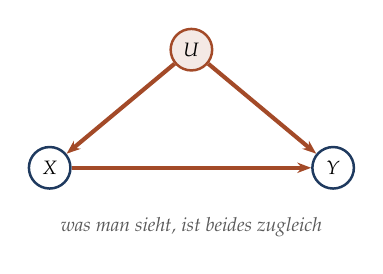
\begin{tikzpicture}[scale=1.0, every node/.style={font=\small}]
\node[knotenr] (u) at (0,1.5) {$U$};
\node[knotenb] (x) at (-1.8,0) {$X$};
\node[knotenb] (y) at (1.8,0) {$Y$};
\draw[kanted, -{Stealth[length=5pt]}] (u)--(x);
\draw[kanted, -{Stealth[length=5pt]}] (u)--(y);
\draw[akzent, line width=1.3pt, -{Stealth[length=5pt]}] (x)--(y);
\node[font=\scriptsize\itshape, color=grau] at (0,-0.75) {was man sieht, ist beides zugleich};
\end{tikzpicture}

\vspace{1.4cm}
{\large\color{grau} Von Simpsons Paradoxon bis zur Zielstudienemulation}\\[6pt]
{\color{grau} Jeder Schritt erklärt. Mit vollständig durchgerechneten Übungsaufgaben.}\\[1.9cm]
{\small\color{grau} Stand der Forschung: August 2026}
\end{titlepage}
\thispagestyle{empty}
\vspace*{\fill}
\begin{flushleft}
{\small\color{grau}
\textbf{\color{tief}Mathematik von Grund auf} --- Band 23\\[2pt]
\textit{Woran es liegt} $\cdot$ Kausale Schlüsse\\[14pt]

Herausgeber und Urheber: Jürgen Maier\\[2pt]
Entstanden 2026 in Zusammenarbeit mit Claude (Anthropic); Konzeption, Vorgaben, Prüfung und Herausgeberschaft: Jürgen Maier.\\[14pt]

\textbf{Lizenz}\\[2pt]
Dieses Werk ist lizenziert unter einer Creative-Commons-Lizenz \textbf{Namensnennung -- Weitergabe unter gleichen Bedingungen 4.0 International (CC BY-SA 4.0)}. Sie dürfen das Werk vervielfältigen, verbreiten, bearbeiten und auch kommerziell nutzen, sofern Sie den Urheber nennen und Bearbeitungen unter derselben Lizenz weitergeben.\\[2pt]
Lizenztext: \texttt{https://creativecommons.org/licenses/by-sa/4.0/legalcode.de}\\[14pt]

\textbf{Quellen und Fassungen}\\[2pt]
Quelltexte, Simulationen, Fehlermeldungen und aktuelle Fassungen aller Bände:\\
\texttt{https://github.com/juergenmaier2026/mathematik-von-grund-auf}\\[2pt]
Dauerhaft archiviert bei Zenodo: \texttt{https://doi.org/10.5281/zenodo.23698547}\\[14pt]

\textbf{Zitiervorschlag}\\[2pt]
Maier, J. (2026). \textit{Mathematik von Grund auf, Band 23: Woran es liegt}. Fassung 1.0.1. \texttt{https://doi.org/10.5281/zenodo.23698547}\\[14pt]

Satz: \LaTeX{} mit Palatino. Fassung 1.0.1, Oktober 2026. 158 Seiten.
}
\end{flushleft}
\vspace*{1.5cm}

\tableofcontents
\mainmatter

\chapter*{Vorwort}
\addcontentsline{toc}{chapter}{Vorwort}

\begin{merksatz}
\boxtitel{Die Frage, die Band 22 offenließ}
Das letzte Kapitel von Band 22 endete mit einer Feststellung: Ein Verfahren, das gut vorhersagt, hat nicht verstanden, warum. Die Merkmale, die es benutzt, beschreiben die Daten --- nicht die Krankheit.

\begin{center}
\begin{minipage}{0.9\textwidth}
\textbf{Dieser Band behandelt die andere Frage: Was geschieht, wenn man eingreift?}
\end{minipage}
\end{center}

\begin{center}
\begin{minipage}{0.88\textwidth}
\kursiv{Sie ist die eigentliche Frage der Medizin. \textbf{Kein Arzt will wissen, welche Patienten sterben werden --- er will wissen, was er tun soll}, damit sie es nicht tun. Das ist keine Frage nach Zusammenhängen, sondern nach Wirkungen, und bis vor wenigen Jahrzehnten galt sie als außerhalb der Statistik liegend.}
\end{minipage}
\end{center}
\end{merksatz}

\begin{merksatz}
\boxtitel{Wo der Band steht}
\begin{center}
{\small
\renewcommand{\arraystretch}{1.52}
\begin{tabular}{@{}P{2.2cm}P{6.4cm}@{}}
\toprule
\textbf{Band 17} & Statistik schätzt Größen einer Verteilung und prüft Hypothesen darüber.\\
\textbf{Band 22} & Das Lernen sagt vorher, was bei einem neuen Fall zu erwarten ist.\\
\textbf{Band 21} & Die Spieltheorie fragt, was geschieht, wenn andere auf eine Änderung reagieren.\\
\textbf{Hier} & Die Frage lautet: Was wäre geschehen, wenn man anders gehandelt hätte?\\
\bottomrule
\end{tabular}}
\end{center}

\begin{center}
\begin{minipage}{0.88\textwidth}
\kursiv{\textbf{Die letzte Zeile enthält eine Größe, die niemand beobachten kann.} Ein Patient wurde früh behandelt oder spät, nicht beides. Was mit ihm im anderen Fall geschehen wäre, ist keine fehlende Messung, sondern eine, die es nicht geben kann. Dass sich über solche Größen dennoch rechnen lässt --- unter angebbaren Annahmen ---, ist der Inhalt dieses Bandes.}
\end{minipage}
\end{center}
\end{merksatz}

\begin{merksatz}
\boxtitel{Drei Ergebnisse, die man nicht erwartet}
\begin{center}
{\small
\renewcommand{\arraystretch}{1.55}
\begin{tabular}{@{}P{1.0cm}P{7.4cm}@{}}
\toprule
$1$ & Dieselbe Tabelle von Zahlen ist mit \kursiv{entgegengesetzten} Wirkungen vereinbar. Keine noch so große Datenmenge kann zwischen ihnen entscheiden --- nur Annahmen können es. \kursiv{(Kapitel 1)}\\
$2$ & Für manche Merkmale ist es ein Fehler, sie herauszurechnen. Wer nach allem anpasst, was er gemessen hat, erzeugt Verzerrungen, die vorher nicht da waren. \kursiv{(Kapitel 5)}\\
$3$ & Aus reinen Beobachtungsdaten lässt sich unter prüfbaren Bedingungen dasselbe berechnen wie aus einer randomisierten Studie --- und die Bedingungen sind erstaunlich oft erfüllt. \kursiv{(Kapitel 6 und 11)}\\
\bottomrule
\end{tabular}}
\end{center}

\begin{center}
\begin{minipage}{0.88\textwidth}
\kursiv{Das zweite Ergebnis widerspricht der verbreiteten Übung, in ein Modell möglichst viele Störgrößen aufzunehmen. \textbf{Es gibt Merkmale, deren Berücksichtigung schadet} --- und man erkennt sie nicht an den Daten, sondern nur an einer Überlegung darüber, wie die Daten entstanden sind.}
\end{minipage}
\end{center}
\end{merksatz}

\begin{merksatz}
\boxtitel{Die sechs Teile}
\begin{center}
{\small
\renewcommand{\arraystretch}{1.5}
\begin{tabular}{@{}P{1.4cm}P{3.4cm}P{3.2cm}@{}}
\toprule
\textbf{Teil} & \textbf{Thema} & \textbf{Kapitel}\\
\midrule
I & Das Problem & $1$--$3$\\
II & Graphen und Regeln & $4$--$6$\\
III & Anpassen & $7$--$8$\\
IV & Wenn Anpassen nicht reicht & $9$--$11$\\
V & Über die Zeit, im Einzelfall & $12$--$14$\\
VI & Stand & $15$\\
\bottomrule
\end{tabular}}
\end{center}

\schritt{Der Leitfall}
Am Klinikum Neustadt zeigen die Behandlungsdaten: \kursiv{Patienten, die früh Antibiotika erhielten, starben häufiger.}

\begin{center}
\begin{minipage}{0.88\textwidth}
\kursiv{Die Leitlinien verlangen eine möglichst frühe Gabe, und die Evidenz dafür ist gut. \textbf{Die eigenen Daten des Hauses scheinen das Gegenteil zu zeigen} --- und die Auflösung dieses Widerspruchs führt durch den ganzen Band. Sie beginnt in Kapitel~1 mit einer Tabelle und endet in Kapitel~11 mit einem Verfahren, das aus Routinedaten eine Studie nachbildet.}
\end{minipage}
\end{center}
\end{merksatz}

\begin{warnung}
\boxtitelr{Drei Warnungen}
\begin{center}
{\small
\renewcommand{\arraystretch}{1.55}
\begin{tabular}{@{}P{2.2cm}P{6.4cm}@{}}
\toprule
\textbf{Erste} & Jede kausale Aussage beruht auf Annahmen, die sich aus den Daten nicht prüfen lassen. Das Verfahren macht sie nicht überflüssig --- es macht sie sichtbar.\\
\textbf{Zweite} & Ein Durchschnittseffekt sagt nichts über den einzelnen Patienten. Er kann positiv sein, während er bei der Hälfte schadet.\\
\textbf{Dritte} & Was in einer Bevölkerung wirkt, muss in einer anderen nicht wirken --- und was unter Studienbedingungen wirkt, nicht im Alltag.\\
\bottomrule
\end{tabular}}
\end{center}

\begin{center}
\begin{minipage}{0.88\textwidth}
\kursiv{Die erste Warnung ist die wichtigste und wird oft für einen Einwand gehalten. \textbf{Sie ist das Gegenteil}: Die Stärke der Verfahren dieses Bandes liegt darin, dass sie die Annahmen benennen, statt sie zu verstecken. Wer eine Regression rechnet und von \enquote{Einfluss} spricht, hat dieselben Annahmen gemacht --- nur ohne sie aufzuschreiben.}
\end{minipage}
\end{center}
\end{warnung}

\begin{merksatz}
\boxtitel{Was dieser Band voraussetzt}
\begin{center}
{\small
\renewcommand{\arraystretch}{1.48}
\begin{tabular}{@{}P{3.0cm}P{1.6cm}P{3.0cm}@{}}
\toprule
\textbf{Werkzeug} & \textbf{Band} & \textbf{gebraucht in}\\
\midrule
Bedingte Wahrscheinlichkeit & $4$ & durchgehend\\
Schätzen, Konfidenz & $17$ & Kapitel 3, 7, 8\\
Regression & $17$, $22$ & Kapitel 7, 9, 14\\
Graphen, Wege & $16$ & Kapitel 4--6\\
Lernverfahren & $22$ & Kapitel 8, 14\\
\bottomrule
\end{tabular}}
\end{center}

\begin{center}
\begin{minipage}{0.88\textwidth}
\kursiv{\textbf{Teil~I und II kommen mit Band 0 und den Grundzügen der Wahrscheinlichkeitsrechnung aus.} Die Graphen aus Band 16 werden gebraucht, aber nur in ihren einfachsten Eigenschaften --- gerichtete Kanten, Wege, Kreisfreiheit. Wo ein Satz aus einem Vorgängerband benutzt wird, steht die Fundstelle dabei.}
\end{minipage}
\end{center}
\end{merksatz}

\part{Das Problem}

\chapter{Zusammenhang und Ursache}

\section{Der Leitfall}

\begin{merksatz}
\boxtitel{Eine Tabelle, die das Gegenteil zeigt}
Am Klinikum Neustadt wurden $1200$ Sepsispatienten ausgewertet. Die Hälfte erhielt das Antibiotikum innerhalb einer Stunde (\enquote{früh}), die andere Hälfte später.

\begin{center}
{\small
\renewcommand{\arraystretch}{1.5}
\begin{tabular}{@{}P{2.4cm}P{2.0cm}P{2.0cm}P{2.2cm}@{}}
\toprule
\textbf{Gabe} & \textbf{Patienten} & \textbf{gestorben} & \textbf{Anteil}\\
\midrule
früh & $600$ & $210$ & $35{,}0\,\%$\\
spät & $600$ & $125$ & $20{,}8\,\%$\\
\bottomrule
\end{tabular}}
\end{center}

\begin{center}
\begin{minipage}{0.9\textwidth}
\textbf{Die frühe Gabe scheint die Sterblichkeit um vierzehn Prozentpunkte zu erhöhen.}
\end{minipage}
\end{center}

\begin{center}
\begin{minipage}{0.88\textwidth}
\kursiv{Das widerspricht allem, was die Leitlinien sagen. \textbf{Ein Statistiker könnte die Zahlen prüfen, und sie wären richtig} --- der Unterschied ist groß, die Stichprobe ausreichend, das Vertrauensintervall schließt die Null weit aus. Trotzdem ist der Schluss falsch, und dieses Kapitel zeigt, woran das liegt.}
\end{minipage}
\end{center}
\end{merksatz}

\begin{merksatz}
\boxtitel{Dieselben Patienten, nach Schweregrad getrennt}
\begin{center}
{\small
\renewcommand{\arraystretch}{1.5}
\begin{tabular}{@{}P{2.2cm}P{1.8cm}P{1.8cm}P{1.8cm}P{1.6cm}@{}}
\toprule
& \multicolumn{2}{c}{\textbf{früh}} & \multicolumn{2}{c}{\textbf{spät}}\\
& $n$ & \textbf{tot} & $n$ & \textbf{tot}\\
\midrule
schwer krank & $500$ & $200$ & $100$ & $50$\\
& & $40\,\%$ & & $50\,\%$\\
leicht krank & $100$ & $10$ & $500$ & $75$\\
& & $10\,\%$ & & $15\,\%$\\
\bottomrule
\end{tabular}}
\end{center}

\begin{center}
\begin{minipage}{0.9\textwidth}
\textbf{In jeder der beiden Gruppen senkt die frühe Gabe die Sterblichkeit --- von $50$ auf $40$ und von $15$ auf $10$ Prozent.}
\end{minipage}
\end{center}

\schritt{Warum sich das Vorzeichen umkehrt}
\begin{center}
{\small
\renewcommand{\arraystretch}{1.5}
\begin{tabular}{@{}P{2.6cm}P{6.0cm}@{}}
\toprule
\textbf{Wer bekommt früh?} & Die Schwerkranken --- $500$ von $600$. Bei ihnen ist die Diagnose offensichtlich, und man handelt sofort.\\
\textbf{Wer stirbt?} & Ebenfalls die Schwerkranken.\\
\bottomrule
\end{tabular}}
\end{center}

\begin{center}
\begin{minipage}{0.88\textwidth}
\kursiv{Der Schweregrad wirkt auf beides: auf die Behandlung und auf den Ausgang. \textbf{Die Gruppe \enquote{früh} besteht überwiegend aus Schwerkranken, die Gruppe \enquote{spät} überwiegend aus Leichtkranken} --- man vergleicht nicht zwei Behandlungen, sondern zwei Patientengruppen. In der Medizin heißt das \Begriff{Indikationsverzerrung}, und sie ist die häufigste Fehlerquelle bei der Auswertung von Behandlungsdaten.}
\end{minipage}
\end{center}
\end{merksatz}

\begin{merksatz}
\boxtitel{Die richtige Rechnung}
Man fragt: Was wäre geschehen, wenn \kursiv{alle} $1200$ früh behandelt worden wären? Und wenn alle spät?

\schritt{Standardisierung}
Der Anteil Schwerkranker ist $600/1200 = \tfrac12$.

\[ \Pr[\text{Tod} \mid \dops(\text{früh})] = \tfrac12\cdot0{,}40 + \tfrac12\cdot0{,}10 = 0{,}250 \]
\[ \Pr[\text{Tod} \mid \dops(\text{spät})] = \tfrac12\cdot0{,}50 + \tfrac12\cdot0{,}15 = 0{,}325 \]

\begin{center}
{\small
\renewcommand{\arraystretch}{1.5}
\begin{tabular}{@{}P{3.4cm}P{2.6cm}@{}}
\toprule
\textbf{Rechnung} & \textbf{Effekt}\\
\midrule
naiver Vergleich & $+14{,}2$ Punkte\\
standardisiert & $\mathbf{-7{,}5}$ \textbf{Punkte}\\
\bottomrule
\end{tabular}}
\end{center}

\begin{center}
\begin{minipage}{0.9\textwidth}
\textbf{Die frühe Gabe rettet siebeneinhalb von hundert Patienten --- statt vierzehn zu töten.}
\end{minipage}
\end{center}

\begin{center}
\begin{minipage}{0.88\textwidth}
\kursiv{\textbf{Der Schweregrad wird dabei nicht weggelassen, sondern gleichgesetzt}: Man rechnet beide Behandlungen für dieselbe Mischung aus Schwer- und Leichtkranken durch. Kapitel~6 wird zeigen, unter welcher Bedingung diese Rechnung erlaubt ist --- und Kapitel~5, dass es Größen gibt, bei denen man sie gerade nicht anwenden darf.}
\end{minipage}
\end{center}
\end{merksatz}

\section{Drei Gründe für einen Zusammenhang}

\begin{merksatz}
\boxtitel{Wenn $X$ und $Y$ zusammenhängen}
\begin{center}
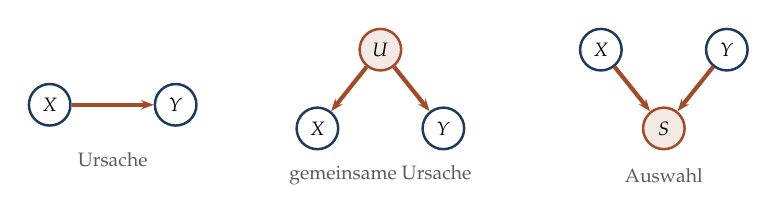
\begin{tikzpicture}[scale=1.0, every node/.style={font=\small}]
\node[knotenb] (x1) at (0,1.2) {$X$}; \node[knotenb] (y1) at (1.6,1.2) {$Y$};
\draw[kanted, -{Stealth[length=4.5pt]}] (x1)--(y1);
\node[font=\scriptsize, color=grau] at (0.8,0.5) {Ursache};

\node[knotenr] (u) at (4.2,1.9) {$U$};
\node[knotenb] (x2) at (3.4,0.9) {$X$}; \node[knotenb] (y2) at (5.0,0.9) {$Y$};
\draw[kanted, -{Stealth[length=4.5pt]}] (u)--(x2); \draw[kanted, -{Stealth[length=4.5pt]}] (u)--(y2);
\node[font=\scriptsize, color=grau] at (4.2,0.3) {gemeinsame Ursache};

\node[knotenb] (x3) at (7.0,1.9) {$X$}; \node[knotenb] (y3) at (8.6,1.9) {$Y$};
\node[knotenr] (s) at (7.8,0.9) {$S$};
\draw[kanted, -{Stealth[length=4.5pt]}] (x3)--(s); \draw[kanted, -{Stealth[length=4.5pt]}] (y3)--(s);
\node[font=\scriptsize, color=grau] at (7.8,0.3) {Auswahl};
\end{tikzpicture}
\end{center}

\begin{center}
{\small
\renewcommand{\arraystretch}{1.55}
\begin{tabular}{@{}P{2.6cm}P{6.0cm}@{}}
\toprule
\textbf{Ursache} & $X$ wirkt auf $Y$. Nur hier hilft ein Eingriff.\\
\textbf{Gemeinsame Ursache} & Eine dritte Größe wirkt auf beide. Man nennt sie \Begriff{Störgröße}. Das ist der Leitfall.\\
\textbf{Auswahl} & Beide wirken auf etwas Drittes, und man betrachtet nur Fälle mit bestimmtem Wert davon. Man nennt das einen \Begriff{Kollider}.\\
\bottomrule
\end{tabular}}
\end{center}

\begin{center}
\begin{minipage}{0.9\textwidth}
\textbf{Alle drei erzeugen denselben Zusammenhang in den Daten. Nur der erste rechtfertigt ein Handeln.}
\end{minipage}
\end{center}

\begin{center}
\begin{minipage}{0.88\textwidth}
\kursiv{Die dritte Zeile ist die unbekannteste und in der klinischen Forschung die tückischste. \textbf{Wer nur stationäre Patienten untersucht, hat bereits nach einem Kollider ausgewählt} --- eine Aufnahme wird durch jedes ernste Leiden begünstigt. Aufgabe 1.2 rechnet vor, wie stark der Zusammenhang wird, den diese Auswahl allein erzeugt.}
\end{minipage}
\end{center}
\end{merksatz}

\section{Zwei Verteilungen}

\begin{definition}
\boxtitelm{Definition 1.1 --- sehen und tun}
\begin{center}
{\small
\renewcommand{\arraystretch}{1.55}
\begin{tabular}{@{}P{2.4cm}P{6.2cm}@{}}
\toprule
$\Pr[Y \mid X = x]$ & \textbf{Sehen:} Wie sieht $Y$ aus \kursiv{unter denen}, bei denen $X$ den Wert $x$ hat?\\
$\Pr[Y \mid \dops(X=x)]$ & \textbf{Tun:} Wie sähe $Y$ aus, wenn man bei \kursiv{allen} den Wert $x$ herstellte?\\
\bottomrule
\end{tabular}}
\end{center}
\end{definition}

\begin{merksatz}
\boxtitel{Der Unterschied}
\begin{center}
{\small
\renewcommand{\arraystretch}{1.5}
\begin{tabular}{@{}P{2.4cm}P{6.2cm}@{}}
\toprule
\textbf{Sehen} & ändert nichts an der Welt. Die Auswahl der Patienten mit $X=x$ ist nicht zufällig.\\
\textbf{Tun} & ändert die Welt: Alle Pfeile, die auf $X$ zeigen, werden durchtrennt. $X$ hängt dann von nichts mehr ab.\\
\bottomrule
\end{tabular}}
\end{center}

\begin{center}
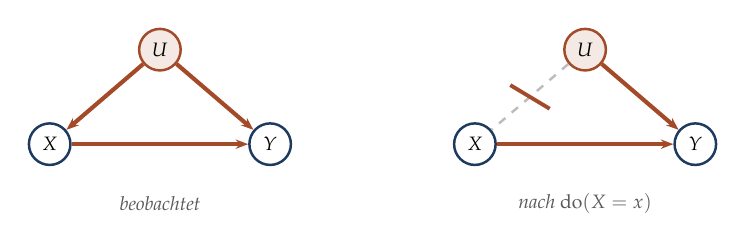
\begin{tikzpicture}[scale=1.0, every node/.style={font=\small}]
\node[knotenr] (u) at (0,1.4) {$U$};
\node[knotenb] (x) at (-1.4,0.2) {$X$}; \node[knotenb] (y) at (1.4,0.2) {$Y$};
\draw[kanted, -{Stealth[length=4.5pt]}] (u)--(x); \draw[kanted, -{Stealth[length=4.5pt]}] (u)--(y);
\draw[kanted, -{Stealth[length=4.5pt]}] (x)--(y);
\node[font=\scriptsize\itshape, color=grau] at (0,-0.55) {beobachtet};

\node[knotenr] (u2) at (5.4,1.4) {$U$};
\node[knotenb] (x2) at (4.0,0.2) {$X$}; \node[knotenb] (y2) at (6.8,0.2) {$Y$};
\draw[grau!40, line width=0.9pt, dashed] (u2)--(x2);
\draw[akzent, line width=1.4pt] (4.45,0.95) -- (4.95,0.65);
\draw[kanted, -{Stealth[length=4.5pt]}] (u2)--(y2);
\draw[kanted, -{Stealth[length=4.5pt]}] (x2)--(y2);
\node[font=\scriptsize\itshape, color=grau] at (5.4,-0.55) {nach $\dops(X=x)$};
\end{tikzpicture}
\end{center}

\begin{center}
\begin{minipage}{0.9\textwidth}
\textbf{Der Eingriff schneidet die Pfeile ab, die in $X$ hineinlaufen --- und nur diese.}
\end{minipage}
\end{center}

\begin{center}
\begin{minipage}{0.88\textwidth}
\kursiv{Im Leitfall heißt das: Der Pfeil \enquote{Schweregrad $\to$ frühe Gabe} verschwindet, der Pfeil \enquote{Schweregrad $\to$ Tod} bleibt. \textbf{Genau das tut eine randomisierte Studie}: Das Los ersetzt die ärztliche Entscheidung und trennt die Behandlung von allem, was sie sonst beeinflusst. Kapitel~3 behandelt das ausführlich.}
\end{minipage}
\end{center}
\end{merksatz}

\section{Warum keine Statistik allein genügt}

\begin{merksatz}
\boxtitel{Satz 1.2 --- Beobachtungsäquivalenz}
Es gibt zwei verschiedene Ursachenstrukturen, die \kursiv{genau dieselbe} gemeinsame Verteilung von $X$ und $Y$ erzeugen --- und in denen der Effekt eines Eingriffs verschieden ist.

\schritt{Die Zahlen}
\begin{center}
{\small
\renewcommand{\arraystretch}{1.5}
\begin{tabular}{@{}P{2.4cm}P{2.2cm}P{2.2cm}@{}}
\toprule
& $Y=1$ & $Y=0$\\
\midrule
$X=1$ & $0{,}40$ & $0{,}10$\\
$X=0$ & $0{,}10$ & $0{,}40$\\
\bottomrule
\end{tabular}}
\end{center}
\[ \Pr[Y=1 \mid X=1] = 0{,}80, \qquad \Pr[Y=1 \mid X=0] = 0{,}20 \]

\schritt{Modell A --- $X$ wirkt auf $Y$}
$X$ ist ein Münzwurf; danach ist $Y=1$ mit Wahrscheinlichkeit $0{,}8$ falls $X=1$, sonst mit $0{,}2$.

\[ \Pr[Y=1\mid\dops(X=1)] = 0{,}80, \qquad \Pr[Y=1\mid\dops(X=0)] = 0{,}20 \]
\[ \text{Effekt} = +0{,}60 \]

\schritt{Modell B --- eine gemeinsame Ursache, $X$ wirkt nicht}
$U$ ist ein Münzwurf. Bei $U=1$ ist $X=1$ mit Wahrscheinlichkeit $a = 0{,}8873$ und unabhängig davon $Y=1$ mit derselben Wahrscheinlichkeit; bei $U=0$ jeweils $1-a$.

\kursiv{Probe:}
\[ \Pr[X=1,Y=1] = \tfrac12 a^{2} + \tfrac12(1-a)^{2} = \tfrac12(0{,}7873) + \tfrac12(0{,}0127) = 0{,}40 \quad \checkmark \]

\[ \Pr[Y=1\mid\dops(X=1)] = \Pr[Y=1\mid\dops(X=0)] = 0{,}50 \]
\[ \text{Effekt} = 0 \]

\begin{center}
\begin{minipage}{0.9\textwidth}
\textbf{Dieselben Zahlen, ein Effekt von $+0{,}60$ oder von null. Kein Test an diesen Daten kann entscheiden, welcher gilt.}
\end{minipage}
\end{center}

\begin{center}
\begin{minipage}{0.88\textwidth}
\kursiv{\textbf{Das ist das erste der drei überraschenden Ergebnisse des Vorworts}, und es ist kein Grenzfall, sondern die Regel: Zu praktisch jeder beobachteten Verteilung gibt es mehrere Ursachenstrukturen. Auch beliebig viele weitere Patienten ändern daran nichts --- sie bestimmen die Verteilung genauer, und die Verteilung ist es ja gerade, die nicht entscheidet.}
\end{minipage}
\end{center}

\schritt{Was daraus folgt}
\begin{center}
{\small
\renewcommand{\arraystretch}{1.5}
\begin{tabular}{@{}P{2.6cm}P{6.0cm}@{}}
\toprule
\textbf{Nicht:} & \enquote{Kausale Schlüsse sind unmöglich.}\\
\textbf{Sondern:} & Sie brauchen Annahmen, die nicht aus den Daten stammen --- aus Fachwissen, aus dem Ablauf in der Zeit, aus dem Versuchsaufbau.\\
\bottomrule
\end{tabular}}
\end{center}

\begin{center}
\begin{minipage}{0.88\textwidth}
\kursiv{\textbf{Das ist genau dieselbe Lage wie in Band 22, Satz 1.5}: Ohne Annahme kein Lernen, ohne Annahme kein kausaler Schluss. Der Unterschied liegt darin, dass die Annahmen hier viel gezielter eingreifen --- und dass die Verfahren dieses Bandes sie aufschreiben statt verschweigen.}
\end{minipage}
\end{center}
\end{merksatz}

\section{Der Bruchfall}

\begin{warnung}
\boxtitelr{Was die Standardisierung voraussetzt}
Die Rechnung in Abschnitt 1.1 war richtig --- unter einer Bedingung, die in den Zahlen nicht steht.

\begin{center}
{\small
\renewcommand{\arraystretch}{1.52}
\begin{tabular}{@{}P{2.6cm}P{6.0cm}@{}}
\toprule
\textbf{Alles gemessen} & Der Schweregrad darf nicht die einzige Störgröße sein, die es gibt --- er muss die einzige sein, die es gibt.\\
\textbf{Zwei Stufen} & \enquote{Schwer} und \enquote{leicht} sind eine grobe Einteilung. Innerhalb der Schwerkranken kann derselbe Zusammenhang erneut auftreten.\\
\textbf{Überlappung} & In jeder Gruppe müssen beide Behandlungen vorkommen. Bei $100$ Prozent früh in einer Gruppe gibt es nichts zu vergleichen.\\
\bottomrule
\end{tabular}}
\end{center}

\begin{center}
\begin{minipage}{0.88\textwidth}
\kursiv{Die erste Zeile ist unprüfbar. \textbf{Man kann nie ausschließen, dass eine weitere, nicht gemessene Größe beides beeinflusst} --- etwa die Erfahrung des diensthabenden Arztes oder die Tageszeit. Kapitel~6 gibt der Annahme einen Namen und eine grafische Fassung; Kapitel~9 und 10 zeigen Wege, die ohne sie auskommen.}
\end{minipage}
\end{center}

\schritt{Und die zweite Zeile in Zahlen}
\begin{center}
\begin{minipage}{0.88\textwidth}
\kursiv{Teilt man \enquote{schwer} nochmals in zwei Stufen, so kann sich das Vorzeichen abermals umkehren --- Simpsons Paradoxon kann sich auf jeder Ebene wiederholen. \textbf{Feinere Einteilung hilft nur, wenn genug Patienten je Stufe bleiben}, sonst tauscht man Verzerrung gegen Varianz, genau wie in Band 22, Kapitel~2. Kapitel~7 behandelt diesen Zielkonflikt.}
\end{minipage}
\end{center}
\end{warnung}

\section{Übungsaufgaben}

\begin{aufgabe}
\boxtitel{Aufgabe 1.1 --- Simpson erzeugen}
Zeigen Sie, wie man aus zwei Untergruppen, in denen die Behandlung jeweils \kursiv{schadet}, eine Gesamttabelle erzeugt, in der sie zu nützen scheint.

\loesung
\schritt{Schritt 1 --- Das Rezept}
Man braucht zwei Bedingungen:
\begin{center}
{\small
\renewcommand{\arraystretch}{1.5}
\begin{tabular}{@{}P{1.0cm}P{7.4cm}@{}}
\toprule
$1$ & Die Untergruppen unterscheiden sich stark im Ausgang.\\
$2$ & Die Behandlung ist in der \kursiv{günstigeren} Untergruppe überrepräsentiert.\\
\bottomrule
\end{tabular}}
\end{center}

\schritt{Schritt 2 --- Zahlen}
\begin{center}
{\small
\renewcommand{\arraystretch}{1.48}
\begin{tabular}{@{}P{2.2cm}P{1.6cm}P{1.6cm}P{1.6cm}P{1.6cm}@{}}
\toprule
& \multicolumn{2}{c}{\textbf{behandelt}} & \multicolumn{2}{c}{\textbf{nicht}}\\
& $n$ & \textbf{tot} & $n$ & \textbf{tot}\\
\midrule
leicht & $900$ & $90$ & $100$ & $5$\\
& & $10\,\%$ & & $5\,\%$\\
schwer & $100$ & $60$ & $900$ & $450$\\
& & $60\,\%$ & & $50\,\%$\\
\midrule
gesamt & $1000$ & $150$ & $1000$ & $455$\\
& & $\mathbf{15\,\%}$ & & $\mathbf{45{,}5\,\%}$\\
\bottomrule
\end{tabular}}
\end{center}

\begin{center}
\begin{minipage}{0.9\textwidth}
\textbf{In beiden Gruppen schadet die Behandlung um zehn Punkte. Insgesamt scheint sie um dreißig Punkte zu nützen.}
\end{minipage}
\end{center}

\schritt{Schritt 3 --- Die standardisierte Rechnung}
Jede Gruppe umfasst $1000$ von $2000$ Patienten, also je die Hälfte:
\[ \Pr[\text{Tod}\mid\dops(\text{behandelt})] = \tfrac12\cdot0{,}10 + \tfrac12\cdot0{,}60 = 0{,}350 \]
\[ \Pr[\text{Tod}\mid\dops(\text{nicht})] = \tfrac12\cdot0{,}05 + \tfrac12\cdot0{,}50 = 0{,}275 \]
\[ \text{Effekt} = +0{,}075 \]

\begin{center}
\begin{minipage}{0.88\textwidth}
\kursiv{\textbf{Die Behandlung schadet um siebeneinhalb Punkte} --- obwohl die Gesamttabelle einen Nutzen von dreißig Punkten zeigt. Der naive Vergleich liegt um $37{,}5$ Punkte daneben und im Vorzeichen falsch.}
\end{minipage}
\end{center}

\schritt{Schritt 4 --- Die Warnung}
\begin{center}
\begin{minipage}{0.88\textwidth}
\kursiv{Man beachte, dass die standardisierte Rechnung hier eine \kursiv{Entscheidung} enthält: Man mittelt über die Hälfte-Hälfte-Mischung der beiden Gruppen. \textbf{Bei anderer Mischung ergäbe sich eine andere Zahl} --- bei lauter Leichtkranken $+5$ Punkte, bei lauter Schwerkranken $+10$. Ein Durchschnittseffekt gilt immer für eine bestimmte Bevölkerung; welche das ist, muss man dazusagen. Das ist die dritte Warnung des Vorworts.}
\end{minipage}
\end{center}
\end{aufgabe}

\begin{aufgabe}
\boxtitel{Aufgabe 1.2 --- Zusammenhang aus reiner Auswahl}
Zwei Leiden $A$ und $B$ treten in der Bevölkerung mit je zehn Prozent auf und sind \kursiv{voneinander unabhängig}. Jedes erhöht die Wahrscheinlichkeit einer Krankenhausaufnahme.

\begin{center}
{\small
\renewcommand{\arraystretch}{1.48}
\begin{tabular}{@{}P{3.0cm}P{2.6cm}@{}}
\toprule
\textbf{Zustand} & \textbf{Aufnahme}\\
\midrule
weder $A$ noch $B$ & $2\,\%$\\
nur eines & $30\,\%$\\
beide & $60\,\%$\\
\bottomrule
\end{tabular}}
\end{center}
Wie hängen $A$ und $B$ unter den Aufgenommenen zusammen?

\loesung
\schritt{Schritt 1 --- Die gemeinsamen Wahrscheinlichkeiten}
\begin{center}
{\small
\renewcommand{\arraystretch}{1.48}
\begin{tabular}{@{}P{2.4cm}P{2.4cm}P{1.8cm}P{2.2cm}@{}}
\toprule
\textbf{Zustand} & \textbf{Anteil} & \textbf{Aufn.} & \textbf{beides}\\
\midrule
kein Leiden & $0{,}81$ & $0{,}02$ & $0{,}0162$\\
nur $A$ & $0{,}09$ & $0{,}30$ & $0{,}0270$\\
nur $B$ & $0{,}09$ & $0{,}30$ & $0{,}0270$\\
$A$ und $B$ & $0{,}01$ & $0{,}60$ & $0{,}0060$\\
\midrule
\textbf{Summe} & $1{,}00$ & & $\mathbf{0{,}0762}$\\
\bottomrule
\end{tabular}}
\end{center}

\schritt{Schritt 2 --- Unter den Aufgenommenen}
\[ \Pr[B \mid A,\ \text{aufgenommen}] = \frac{0{,}0060}{0{,}0270+0{,}0060} = \frac{0{,}0060}{0{,}0330} = 0{,}182 \]
\[ \Pr[B \mid \text{nicht } A,\ \text{aufgenommen}] = \frac{0{,}0270}{0{,}0162+0{,}0270} = \frac{0{,}0270}{0{,}0432} = 0{,}625 \]

\begin{center}
\begin{minipage}{0.9\textwidth}
\textbf{Unter den Aufgenommenen haben Patienten mit $A$ deutlich \kursiv{seltener} auch $B$ --- $18$ gegen $63$ Prozent.}
\end{minipage}
\end{center}

\schritt{Schritt 3 --- Das Chancenverhältnis}
\[ \frac{0{,}182/0{,}818}{0{,}625/0{,}375} = \frac{0{,}222}{1{,}667} = 0{,}133 \]

\begin{center}
\begin{minipage}{0.9\textwidth}
\textbf{Ein Chancenverhältnis von $0{,}13$ --- in einer Bevölkerung, in der die beiden Leiden nichts miteinander zu tun haben.}
\end{minipage}
\end{center}

\schritt{Schritt 4 --- Die Deutung}
\begin{center}
\begin{minipage}{0.88\textwidth}
\kursiv{Wer aufgenommen ist und kein $A$ hat, muss einen anderen Grund haben --- meist $B$. \textbf{Das Wissen um die Aufnahme macht die beiden Leiden gegenseitig erklärend}, und deshalb schließt das eine das andere aus. Der Effekt heißt nach \Person{Joseph Berkson}, der ihn 1946 an Krankenhausdaten beschrieb.}
\end{minipage}
\end{center}

\schritt{Schritt 5 --- Die praktische Folge}
\begin{center}
\begin{minipage}{0.88\textwidth}
\kursiv{\textbf{Jede Studie an stationären Patienten hat nach einem Kollider ausgewählt.} Findet sie einen Zusammenhang zwischen zwei Erkrankungen, so kann er ganz oder teilweise aus der Auswahl stammen --- und zwar mit umgekehrtem Vorzeichen gegenüber der Wirklichkeit. Dasselbe gilt für Studien an Freiwilligen, an Versicherten oder an Patienten mit vollständiger Dokumentation.}
\end{minipage}
\end{center}
\end{aufgabe}

\begin{aufgabe}
\boxtitel{Aufgabe 1.3 --- Sehen und tun rechnen}
Prüfen Sie in Modell B aus Satz 1.2 nach, dass $\Pr[Y=1\mid X=1] = 0{,}80$ ist, aber $\Pr[Y=1\mid\dops(X=1)] = 0{,}50$.

\loesung
\schritt{Schritt 1 --- Das Modell}
\begin{center}
{\small
\renewcommand{\arraystretch}{1.48}
\begin{tabular}{@{}P{1.6cm}P{2.0cm}P{2.4cm}P{2.4cm}@{}}
\toprule
$U$ & $\Pr[U]$ & $\Pr[X=1\mid U]$ & $\Pr[Y=1\mid U]$\\
\midrule
$1$ & $0{,}5$ & $0{,}8873$ & $0{,}8873$\\
$0$ & $0{,}5$ & $0{,}1127$ & $0{,}1127$\\
\bottomrule
\end{tabular}}
\end{center}
$X$ und $Y$ sind bei gegebenem $U$ unabhängig --- kein Pfeil von $X$ nach $Y$.

\schritt{Schritt 2 --- Sehen}
\[ \Pr[X=1,Y=1] = 0{,}5\cdot0{,}8873^{2} + 0{,}5\cdot0{,}1127^{2} = 0{,}3937 + 0{,}0063 = 0{,}400 \]
\[ \Pr[X=1] = 0{,}5\cdot0{,}8873 + 0{,}5\cdot0{,}1127 = 0{,}500 \]
\[ \Pr[Y=1 \mid X=1] = \frac{0{,}400}{0{,}500} = 0{,}800 \quad \checkmark \]

\schritt{Schritt 3 --- Tun}
Der Eingriff setzt $X$ auf $1$ und durchtrennt den Pfeil von $U$ nach $X$. An der Verteilung von $Y$ ändert das nichts, denn $Y$ hängt nur von $U$ ab:
\[ \Pr[Y=1\mid\dops(X=1)] = \Pr[Y=1] = 0{,}5\cdot0{,}8873 + 0{,}5\cdot0{,}1127 = 0{,}500 \quad \checkmark \]

\schritt{Schritt 4 --- Der Vergleich}
\begin{center}
{\small
\renewcommand{\arraystretch}{1.5}
\begin{tabular}{@{}P{2.6cm}P{2.2cm}P{2.2cm}@{}}
\toprule
& $X=1$ & $X=0$\\
\midrule
sehen & $0{,}800$ & $0{,}200$\\
tun & $0{,}500$ & $0{,}500$\\
\bottomrule
\end{tabular}}
\end{center}

\begin{center}
\begin{minipage}{0.88\textwidth}
\kursiv{\textbf{Das Sehen zeigt einen Unterschied von $0{,}6$, das Tun keinen.} Der beobachtete Zusammenhang ist vollständig durch $U$ erklärt: Wer $X=1$ hat, hatte wahrscheinlich $U=1$, und wer $U=1$ hatte, hat wahrscheinlich $Y=1$. Man sieht an $X$ etwas über $U$ --- aber man ändert durch $X$ nichts an $U$.}
\end{minipage}
\end{center}

\schritt{Schritt 5 --- Die Merkregel}
\begin{center}
\begin{minipage}{0.9\textwidth}
\textbf{Beobachten heißt: erfahren, welche Welt vorliegt. Eingreifen heißt: eine neue Welt herstellen.}
\end{minipage}
\end{center}
\end{aufgabe}

\begin{geschichte}
\boxtitelg{Ein Paradoxon mit drei Namen}
\Person{Edward Simpson} beschrieb 1951 die Umkehr, die dieses Kapitel eröffnet --- allerdings hatten \Person{Karl Pearson} 1899 und \Person{Udny Yule} 1903 dasselbe Phänomen bereits behandelt.

\begin{center}
\begin{minipage}{0.9\textwidth}
\kursiv{Simpson selbst nannte es kein Paradoxon; er hielt fest, dass die Frage, welche Tabelle die richtige sei, \kursiv{nicht} statistisch zu entscheiden ist, sondern vom Sachzusammenhang abhängt. \textbf{Damit hatte er die Lehre dieses Bandes bereits 1951 formuliert} --- und sie wurde ein halbes Jahrhundert lang überlesen.}
\end{minipage}
\end{center}

\schritt{Ein berühmter Fall}
1973 schien die Universität Berkeley Frauen bei der Zulassung zu benachteiligen: $44$ Prozent der Männer wurden angenommen, aber nur $35$ Prozent der Frauen.

\begin{center}
\begin{minipage}{0.9\textwidth}
\kursiv{Nach Fachbereichen getrennt kehrte sich das Bild in den meisten Fächern um. Frauen hatten sich häufiger für Fächer mit niedrigen Annahmequoten beworben. \textbf{Ob das die Benachteiligung widerlegt oder nur verschiebt, ist eine kausale Frage} --- womöglich war die Fächerwahl selbst eine Folge früherer Benachteiligung. Die Zahlen allein entscheiden es nicht.}
\end{minipage}
\end{center}

\schritt{Und der Widerstand}
\begin{center}
\begin{minipage}{0.9\textwidth}
\kursiv{\Person{Ronald Fisher} bestritt bis zu seinem Tod 1962, dass der Zusammenhang zwischen Rauchen und Lungenkrebs ursächlich sei; er hielt eine gemeinsame genetische Ursache für möglich. \textbf{Sein Einwand war logisch korrekt} --- Satz 1.2 gibt ihm recht --- und in der Sache falsch. Die Antwort kam nicht aus der Statistik, sondern aus Dosis-Wirkungs-Beziehungen, Tierversuchen und der Beobachtung, dass Aufhören das Risiko senkt.}
\end{minipage}
\end{center}
\end{geschichte}

\begin{forschung}
\boxtitelp{Kausalität heute}
\begin{center}
{\small
\renewcommand{\arraystretch}{1.45}
\begin{tabular}{@{}P{2.8cm}P{5.4cm}@{}}
\toprule
\textbf{Routinedaten} & Aus Krankenakten Behandlungseffekte schätzen --- Kapitel~11.\\
\textbf{Ursachen entdecken} & Aus Daten die Struktur selbst gewinnen, nicht nur Effekte schätzen.\\
\textbf{Lernen und Kausalität} & Verfahren, die auch bei veränderter Verteilung gelten.\\
\bottomrule
\end{tabular}}
\end{center}

\schritt{Zur dritten Zeile}
\begin{center}
\begin{minipage}{0.88\textwidth}
\kursiv{Band 22 endete mit der offenen Frage, wann ein an einer Klinik gelerntes Verfahren an einer anderen gilt. \textbf{Eine der wenigen belastbaren Antworten lautet: dann, wenn es kausale Zusammenhänge gelernt hat} --- denn diese bleiben unter Eingriffen und Verteilungsverschiebungen stabil, Korrelationen nicht. Das Sepsis-Warnsystem von 2021 scheiterte an einer Verschiebung; ein Modell, das nur auf ursächlichen Größen beruht, wäre robuster gewesen, hätte aber vermutlich schlechter vorhergesagt.}
\end{minipage}
\end{center}
\end{forschung}

\begin{merksatz}
\boxtitel{Was Sie jetzt können}
\begin{center}
\renewcommand{\arraystretch}{1.5}
\begin{tabular}{@{}P{3.0cm}P{5.6cm}@{}}
\toprule
\textbf{Simpson} & das Vorzeichen kann sich umkehren\\
\textbf{Drei Gründe} & Ursache, gemeinsame Ursache, Auswahl\\
\textbf{Definition 1.1} & sehen gegen tun\\
\textbf{Satz 1.2} & dieselben Daten, verschiedene Effekte\\
\textbf{Standardisierung} & über die Störgröße mitteln\\
\bottomrule
\end{tabular}
\end{center}

\begin{center}
\begin{minipage}{0.88\textwidth}
\kursiv{Dieses Kapitel hat den Effekt an einem Beispiel ausgerechnet, ohne ihn zu definieren. Das nächste holt das nach --- mit einer Größe, die für jeden einzelnen Patienten unbeobachtbar ist und für eine Gruppe trotzdem schätzbar.}
\end{minipage}
\end{center}
\end{merksatz}

\chapter{Was gewesen wäre}

\section{Der Leitfall, einzeln betrachtet}

\begin{merksatz}
\boxtitel{Ein Patient}
Herr K., $68$ Jahre, Sepsis, schwer krank. Er erhielt das Antibiotikum nach vierzig Minuten und überlebte.

\begin{center}
\begin{minipage}{0.9\textwidth}
\textbf{Hat die frühe Gabe ihm geholfen?}
\end{minipage}
\end{center}

\begin{center}
\begin{minipage}{0.88\textwidth}
\kursiv{Die Frage ist klar gestellt und dennoch nicht zu beantworten. \textbf{Um sie zu beantworten, müsste man wissen, was mit ihm geschehen wäre, hätte man länger gewartet} --- und das kann niemand wissen, weil es diesen Patienten nur einmal gibt. Dieses Kapitel gibt der unbeobachtbaren Größe einen Namen, zeigt, warum sie für den Einzelnen unerreichbar bleibt, und unter welchen Bedingungen sie für eine Gruppe dennoch schätzbar ist.}
\end{minipage}
\end{center}
\end{merksatz}

\begin{definition}
\boxtitelm{Definition 2.1 --- potentielle Ergebnisse}
Für jeden Patienten $i$ und jede Behandlung $x$ sei
\[ Y_i(x) \]
das Ergebnis, das eintreten \kursiv{würde}, wenn er die Behandlung $x$ erhielte.

Bei zwei Behandlungen hat jeder Patient zwei solche Größen, $Y_i(1)$ und $Y_i(0)$, und der \Begriff{individuelle Effekt} ist
\[ \tau_i = Y_i(1) - Y_i(0) . \]
\end{definition}

\begin{merksatz}
\boxtitel{Was daran neu ist}
\begin{center}
{\small
\renewcommand{\arraystretch}{1.55}
\begin{tabular}{@{}P{2.6cm}P{6.0cm}@{}}
\toprule
\textbf{Bisher} & Eine Zufallsgröße $Y$ nimmt Werte an, und man fragt nach ihrer Verteilung, auch bedingt auf anderes.\\
\textbf{Jetzt} & Jeder Patient trägt \kursiv{zwei} Werte in sich --- einen für jede mögliche Behandlung. Beobachtbar ist immer nur einer.\\
\bottomrule
\end{tabular}}
\end{center}

\schritt{Die Verbindung zum Beobachteten}
\[ Y_i = Y_i(X_i) \]
--- das beobachtete Ergebnis ist dasjenige potentielle Ergebnis, das zur tatsächlich gegebenen Behandlung gehört. Diese Annahme heißt \Begriff{Konsistenz}.

\begin{center}
\begin{minipage}{0.88\textwidth}
\kursiv{Sie klingt selbstverständlich und ist es nicht. \textbf{Sie verlangt, dass \enquote{die Behandlung} eindeutig bestimmt ist}: Wenn \enquote{früh} bei dem einen vierzig Minuten und bei dem anderen fünfzig heißt, so gibt es nicht ein $Y_i(1)$, sondern viele. Der Bruchfall kommt darauf zurück.}
\end{minipage}
\end{center}
\end{merksatz}

\begin{merksatz}
\boxtitel{Satz 2.2 --- das grundlegende Problem}
Der individuelle Effekt $\tau_i$ ist für keinen einzigen Patienten beobachtbar.

\schritt{Begründung}
Man beobachtet $Y_i(1)$ oder $Y_i(0)$, nie beides --- der Patient wurde entweder früh behandelt oder nicht.

\begin{center}
{\small
\renewcommand{\arraystretch}{1.5}
\begin{tabular}{@{}P{1.8cm}P{1.6cm}P{1.8cm}P{1.8cm}@{}}
\toprule
\textbf{Patient} & $X_i$ & $Y_i(1)$ & $Y_i(0)$\\
\midrule
Herr K. & $1$ & \textcolor{gruen}{überlebt} & \textcolor{akzent}{?}\\
Frau L. & $0$ & \textcolor{akzent}{?} & \textcolor{gruen}{gestorben}\\
\bottomrule
\end{tabular}}
\end{center}

\begin{center}
\begin{minipage}{0.9\textwidth}
\textbf{Die Hälfte der Tabelle fehlt --- und zwar unvermeidlich, nicht aus Nachlässigkeit.}
\end{minipage}
\end{center}

\begin{center}
\begin{minipage}{0.88\textwidth}
\kursiv{\Person{Paul Holland} nannte das 1986 das \enquote{grundlegende Problem der kausalen Inferenz}. \textbf{Es ist kein Messproblem, sondern ein begriffliches}: Die fehlende Größe existiert nicht als Tatsache über die Welt, sondern nur als Aussage darüber, was gewesen wäre. Man kann sie nicht nachmessen, auch nicht mit beliebigem Aufwand.}
\end{minipage}
\end{center}
\end{merksatz}

\section{Vom Einzelnen zur Gruppe}

\begin{definition}
\boxtitelm{Definition 2.3 --- Durchschnittseffekte}
\begin{center}
{\small
\renewcommand{\arraystretch}{1.6}
\begin{tabular}{@{}P{2.8cm}P{5.8cm}@{}}
\toprule
$\tau = \mathbb{E}[Y(1)-Y(0)]$ & \textbf{Durchschnittseffekt} über alle.\\
$\tau_{\text{beh}} = \mathbb{E}[Y(1)-Y(0) \mid X=1]$ & \textbf{Effekt bei den Behandelten}.\\
\bottomrule
\end{tabular}}
\end{center}
\end{definition}

\begin{merksatz}
\boxtitel{Warum zwei Größen}
\begin{center}
{\small
\renewcommand{\arraystretch}{1.5}
\begin{tabular}{@{}P{2.6cm}P{6.0cm}@{}}
\toprule
$\tau$ & Was geschähe, wenn man \kursiv{alle} behandelte? Die Frage einer Leitlinie.\\
$\tau_{\text{beh}}$ & Was hat die Behandlung denen gebracht, die sie erhalten haben? Die Frage einer Nachbetrachtung.\\
\bottomrule
\end{tabular}}
\end{center}

\begin{center}
\begin{minipage}{0.88\textwidth}
\kursiv{Beide fallen auseinander, sobald die Behandelten sich von den übrigen unterscheiden --- also fast immer. \textbf{Im Leitfall sind die Behandelten überwiegend schwer krank}; dort kann die Wirkung größer oder kleiner sein als bei den Leichtkranken. Aufgabe 2.1 rechnet beide aus und findet $-0{,}25$ gegen $-0{,}375$.}
\end{minipage}
\end{center}
\end{merksatz}

\section{Vier Annahmen}

\begin{merksatz}
\boxtitel{Was man braucht, um zu rechnen}
\begin{center}
{\small
\renewcommand{\arraystretch}{1.6}
\begin{tabular}{@{}P{2.8cm}P{5.8cm}@{}}
\toprule
\textbf{Konsistenz} & $Y_i = Y_i(X_i)$ --- die Behandlung ist eindeutig bestimmt.\\
\textbf{Keine Wechselwirkung} & Die Behandlung des einen wirkt nicht auf das Ergebnis des anderen.\\
\textbf{Positivität} & In jeder Gruppe kommen beide Behandlungen vor: $0 < \Pr[X=1\mid Z] < 1$.\\
\textbf{Bedingte Unabhängigkeit} & $\bigl(Y(1),Y(0)\bigr) \perp X \mid Z$ --- bei gleichem $Z$ ist die Behandlung so gut wie ausgelost.\\
\bottomrule
\end{tabular}}
\end{center}

\begin{center}
\begin{minipage}{0.9\textwidth}
\textbf{Nur die dritte Annahme lässt sich an den Daten prüfen.}
\end{minipage}
\end{center}

\begin{center}
\begin{minipage}{0.88\textwidth}
\kursiv{Die erste ist eine Frage der Begriffsbildung, die zweite eine des Sachverhalts, die vierte eine des Fachwissens --- und gerade die vierte trägt die ganze Last. \textbf{Sie besagt, dass es außer $Z$ keine gemeinsame Ursache von Behandlung und Ergebnis gibt}, und das ist genau die unprüfbare Annahme aus dem Bruchfall von Kapitel~1. Kapitel~6 gibt ihr eine grafische Gestalt, an der man sie wenigstens diskutieren kann.}
\end{minipage}
\end{center}
\end{merksatz}

\begin{merksatz}
\boxtitel{Satz 2.4 --- die Anpassungsformel}
Unter Konsistenz, Positivität und bedingter Unabhängigkeit gilt
\[ \mathbb{E}\bigl[Y(x)\bigr] = \sum_z \mathbb{E}\bigl[Y \mid X=x,\ Z=z\bigr]\cdot\Pr[Z=z] . \]

\schritt{Beweis}
\kursiv{Erstens --- nach $Z$ zerlegen} (Satz von der totalen Erwartung, Band 4, Kapitel~9):
\[ \mathbb{E}[Y(x)] = \sum_z \mathbb{E}[Y(x) \mid Z=z]\,\Pr[Z=z] \]

\kursiv{Zweitens --- die Behandlung hinzunehmen:} Nach der bedingten Unabhängigkeit ändert die Bedingung auf $X=x$ bei gegebenem $Z=z$ nichts an der Verteilung von $Y(x)$:
\[ \mathbb{E}[Y(x) \mid Z=z] = \mathbb{E}[Y(x) \mid X=x,\ Z=z] \]
Damit dieser Ausdruck überhaupt definiert ist, braucht man die Positivität.

\kursiv{Drittens --- Konsistenz:} Unter denen mit $X=x$ ist $Y(x)$ das beobachtete $Y$:
\[ \mathbb{E}[Y(x) \mid X=x,\ Z=z] = \mathbb{E}[Y \mid X=x,\ Z=z] \]

\kursiv{Einsetzen} liefert die Behauptung. $\blacksquare$

\begin{center}
\begin{minipage}{0.9\textwidth}
\textbf{Jede der drei Annahmen wird in genau einem Schritt gebraucht --- und ohne sie bricht der Beweis an dieser Stelle ab.}
\end{minipage}
\end{center}

\begin{center}
\begin{minipage}{0.88\textwidth}
\kursiv{\textbf{Das ist die Standardisierung aus Kapitel~1}, nun mit Begründung. Sie war dort eine plausible Rechnung; hier ist sie ein Satz mit angebbaren Voraussetzungen. Der Unterschied zwischen beidem ist der Gegenstand dieses Bandes.}
\end{minipage}
\end{center}
\end{merksatz}

\section{Der Bruchfall}

\begin{warnung}
\boxtitelr{Wechselwirkung: der Fall, in dem alles zusammenbricht}
Die zweite Annahme --- die Behandlung des einen wirke nicht auf das Ergebnis des anderen --- ist bei ansteckenden Krankheiten falsch.

\begin{center}
\begin{minipage}{0.88\textwidth}
\kursiv{Wird ein Patient geimpft, so sinkt auch das Risiko seiner Nachbarn. \textbf{Dann gibt es nicht zwei potentielle Ergebnisse je Person, sondern eines für jede denkbare Belegung der ganzen Bevölkerung} --- bei $n$ Personen also $2^{n}$. Definition 2.1 ist dann gar nicht anwendbar.}
\end{minipage}
\end{center}

\schritt{Was man stattdessen tut}
\begin{center}
{\small
\renewcommand{\arraystretch}{1.5}
\begin{tabular}{@{}P{2.6cm}P{6.0cm}@{}}
\toprule
\textbf{Gruppen bilden} & Man randomisiert ganze Dörfer oder Stationen statt einzelner Personen.\\
\textbf{Effekte trennen} & Direkter Effekt der eigenen Impfung, indirekter Effekt der Impfung anderer.\\
\bottomrule
\end{tabular}}
\end{center}

\begin{center}
\begin{minipage}{0.88\textwidth}
\kursiv{\textbf{Der indirekte Effekt ist die Herdenwirkung aus Band 18, Kapitel~7.} Dort wurde sie als Eigenschaft des SIR-Modells hergeleitet; hier erscheint sie als Grund, warum ein ganzes Begriffsgebäude nicht greift. Bei Antibiotika kommt eine zweite Wechselwirkung hinzu: Die Resistenzlage einer Station hängt davon ab, wie andere Patienten behandelt wurden --- Band 21, Kapitel~10.}
\end{minipage}
\end{center}
\end{warnung}

\begin{warnung}
\boxtitelr{Konsistenz: was heißt \enquote{früh}?}
\begin{center}
{\small
\renewcommand{\arraystretch}{1.52}
\begin{tabular}{@{}P{2.6cm}P{6.0cm}@{}}
\toprule
\textbf{Unscharf} & \enquote{Innerhalb einer Stunde} umfasst fünf Minuten und neunundfünfzig.\\
\textbf{Mit Begleitumständen} & Wer früh behandelt wird, bekommt oft auch früher Flüssigkeit und mehr Aufmerksamkeit.\\
\bottomrule
\end{tabular}}
\end{center}

\begin{center}
\begin{minipage}{0.88\textwidth}
\kursiv{Der geschätzte Effekt gilt dann für das Bündel, nicht für das Antibiotikum allein. \textbf{Die Regel lautet: Man muss den Eingriff so genau beschreiben können, dass zwei Ärzte ihn gleich ausführen würden.} Bei Medikamenten gelingt das meist, bei Begriffen wie \enquote{Adipositas} oder \enquote{Stress} nicht --- und deshalb sind kausale Aussagen über solche Größen schwer zu fassen.}
\end{minipage}
\end{center}
\end{warnung}

\section{Übungsaufgaben}

\begin{aufgabe}
\boxtitel{Aufgabe 2.1 --- Die vollständige Tabelle}
Für acht Patienten seien ausnahmsweise \kursiv{beide} potentiellen Ergebnisse bekannt ($1$ bedeutet gestorben):
\begin{center}
{\small
\renewcommand{\arraystretch}{1.44}
\begin{tabular}{@{}P{1.2cm}P{1.8cm}P{1.2cm}P{1.2cm}P{1.0cm}P{1.4cm}@{}}
\toprule
\textbf{Nr.} & \textbf{Schwere} & $Y(0)$ & $Y(1)$ & $X$ & \textbf{$Y$ beob.}\\
\midrule
$1$ & schwer & $1$ & $1$ & $1$ & $1$\\
$2$ & schwer & $1$ & $0$ & $1$ & $0$\\
$3$ & schwer & $1$ & $1$ & $1$ & $1$\\
$4$ & schwer & $1$ & $0$ & $0$ & $1$\\
$5$ & leicht & $0$ & $0$ & $1$ & $0$\\
$6$ & leicht & $1$ & $0$ & $0$ & $1$\\
$7$ & leicht & $0$ & $0$ & $0$ & $0$\\
$8$ & leicht & $0$ & $0$ & $0$ & $0$\\
\bottomrule
\end{tabular}}
\end{center}
Berechnen Sie $\tau$, $\tau_{\text{beh}}$, den naiven Vergleich und die Anpassungsformel.

\loesung
\schritt{Schritt 1 --- Die individuellen Effekte}
\begin{center}
{\small
\renewcommand{\arraystretch}{1.44}
\begin{tabular}{@{}P{1.2cm}P{1.2cm}P{1.2cm}P{1.2cm}P{1.2cm}P{1.2cm}P{1.2cm}P{1.2cm}@{}}
\toprule
$1$ & $2$ & $3$ & $4$ & $5$ & $6$ & $7$ & $8$\\
\midrule
$0$ & $-1$ & $0$ & $-1$ & $0$ & $-1$ & $0$ & $0$\\
\bottomrule
\end{tabular}}
\end{center}

\begin{center}
\begin{minipage}{0.9\textwidth}
\textbf{Bei drei von acht Patienten rettet die Behandlung das Leben, bei fünf ändert sie nichts. Sie schadet niemandem.}
\end{minipage}
\end{center}

\schritt{Schritt 2 --- Die Durchschnittseffekte}
\[ \tau = \frac{-3}{8} = -0{,}375 \]
\kursiv{Behandelt sind $1$, $2$, $3$, $5$:}
\[ \tau_{\text{beh}} = \frac{0-1+0+0}{4} = -0{,}250 \]
\kursiv{Unbehandelt sind $4$, $6$, $7$, $8$:}
\[ \tau_{\text{unbeh}} = \frac{-1-1+0+0}{4} = -0{,}500 \]

\begin{center}
\begin{minipage}{0.88\textwidth}
\kursiv{\textbf{Die Behandlung hätte bei den Unbehandelten doppelt so viel genützt wie bei den Behandelten.} Wer nur $\tau_{\text{beh}}$ berichtet, unterschätzt, was eine allgemeine Leitlinie brächte.}
\end{minipage}
\end{center}

\schritt{Schritt 3 --- Der naive Vergleich}
\[ \bar Y_{X=1} = \frac{1+0+1+0}{4} = 0{,}50, \qquad \bar Y_{X=0} = \frac{1+1+0+0}{4} = 0{,}50 \]
\[ \text{Unterschied} = 0 \]

\begin{center}
\begin{minipage}{0.9\textwidth}
\textbf{Der naive Vergleich zeigt gar keinen Effekt --- der wahre ist $-0{,}375$.}
\end{minipage}
\end{center}

\schritt{Schritt 4 --- Die Anpassungsformel}
\begin{center}
{\small
\renewcommand{\arraystretch}{1.46}
\begin{tabular}{@{}P{1.8cm}P{2.4cm}P{2.4cm}P{1.6cm}@{}}
\toprule
\textbf{Gruppe} & \textbf{behandelt} & \textbf{unbehandelt} & \textbf{Anteil}\\
\midrule
schwer & $2/3 = 0{,}667$ & $1/1 = 1{,}000$ & $0{,}5$\\
leicht & $0/1 = 0{,}000$ & $1/3 = 0{,}333$ & $0{,}5$\\
\bottomrule
\end{tabular}}
\end{center}

\[ \hat\tau = 0{,}5\,(0{,}667-1{,}000) + 0{,}5\,(0{,}000-0{,}333) = -0{,}167 - 0{,}167 = -0{,}333 \]

\begin{center}
\begin{minipage}{0.88\textwidth}
\kursiv{\textbf{Die Anpassung liefert $-0{,}333$ gegen einen wahren Wert von $-0{,}375$} --- der Rest ist Zufall der kleinen Stichprobe, nicht Verzerrung: In jeder Gruppe stehen nur ein bis drei Patienten. Bei $1200$ Patienten wie in Kapitel~1 verschwindet dieser Unterschied.}
\end{minipage}
\end{center}
\end{aufgabe}

\begin{aufgabe}
\boxtitel{Aufgabe 2.2 --- Die Annahme prüfen}
Zeigen Sie an derselben Tabelle, dass die bedingte Unabhängigkeit hier tatsächlich gilt, und was geschähe, wenn sie verletzt wäre.

\loesung
\schritt{Schritt 1 --- Was zu prüfen ist}
Innerhalb jeder Schweregruppe müssten Behandelte und Unbehandelte dieselben potentiellen Ergebnisse haben.

\begin{center}
{\small
\renewcommand{\arraystretch}{1.46}
\begin{tabular}{@{}P{1.8cm}P{2.6cm}P{2.6cm}@{}}
\toprule
\textbf{Gruppe} & $\bar Y(0)$ behandelt & $\bar Y(0)$ unbehandelt\\
\midrule
schwer & $1{,}000$ & $1{,}000$\\
leicht & $0{,}000$ & $0{,}333$\\
\bottomrule
\end{tabular}}
\end{center}

\begin{center}
\begin{minipage}{0.9\textwidth}
\textbf{In der schweren Gruppe stimmen sie überein, in der leichten nicht ganz} --- $0{,}000$ gegen $0{,}333$.
\end{minipage}
\end{center}

\schritt{Schritt 2 --- Ist das eine Verletzung?}
\begin{center}
\begin{minipage}{0.88\textwidth}
\kursiv{Nicht notwendig. Die leichte Gruppe umfasst vier Patienten, davon einen behandelten. \textbf{Ein Unterschied von einem Drittel bei so wenigen Fällen ist mit Zufall vereinbar.} Die Annahme ist eine Aussage über die Verteilung, nicht über die Stichprobe --- und genau deshalb lässt sie sich an der Stichprobe nicht widerlegen.}
\end{minipage}
\end{center}

\schritt{Schritt 3 --- Eine echte Verletzung}
Man tausche die Behandlung der Patienten $5$ und $6$: Nun ist Patient $6$ behandelt (er hätte ohne Behandlung $Y(0)=1$) und Patient $5$ nicht.

\begin{center}
{\small
\renewcommand{\arraystretch}{1.46}
\begin{tabular}{@{}P{1.8cm}P{2.4cm}P{2.4cm}P{1.6cm}@{}}
\toprule
\textbf{Gruppe} & \textbf{behandelt} & \textbf{unbehandelt} & \textbf{Anteil}\\
\midrule
schwer & $0{,}667$ & $1{,}000$ & $0{,}5$\\
leicht & $0/1 = 0{,}000$ & $0/3 = 0{,}000$ & $0{,}5$\\
\bottomrule
\end{tabular}}
\end{center}

\[ \hat\tau = 0{,}5\,(-0{,}333) + 0{,}5\,(0{,}000) = -0{,}167 \]

\begin{center}
\begin{minipage}{0.9\textwidth}
\textbf{Derselbe wahre Effekt von $-0{,}375$, nun auf $-0{,}167$ geschätzt} --- weil innerhalb der leichten Gruppe gerade der Kränkere behandelt wurde.
\end{minipage}
\end{center}

\schritt{Schritt 4 --- Die Lehre}
\begin{center}
\begin{minipage}{0.88\textwidth}
\kursiv{\textbf{Die Anpassung an $Z$ hilft nur, wenn $Z$ alles enthält, wonach ausgewählt wurde.} Hier hat der Arzt innerhalb der leichten Gruppe nach etwas ausgewählt, das nicht in $Z$ steht --- vielleicht dem Aussehen des Patienten. Kein Rechenverfahren kann das bemerken; nur die Frage, woraufhin der Arzt entschieden hat.}
\end{minipage}
\end{center}
\end{aufgabe}

\begin{aufgabe}
\boxtitel{Aufgabe 2.3 --- Positivität}
In einer Klinik erhalten alle Schwerkranken das Antibiotikum früh. Was folgt daraus, und was geschieht bei $98$ statt $100$ Prozent?

\loesung
\schritt{Schritt 1 --- Bei hundert Prozent}
In der Anpassungsformel steht für die schwere Gruppe der Ausdruck
\[ \mathbb{E}[Y \mid X=0,\ Z=\text{schwer}] \]
--- ein Mittelwert über eine leere Menge.

\begin{center}
\begin{minipage}{0.9\textwidth}
\textbf{Der Durchschnittseffekt ist nicht schätzbar.} Nicht ungenau, sondern gar nicht.
\end{minipage}
\end{center}

\schritt{Schritt 2 --- Was trotzdem geht}
\begin{center}
{\small
\renewcommand{\arraystretch}{1.5}
\begin{tabular}{@{}P{2.8cm}P{5.8cm}@{}}
\toprule
\textbf{Andere Zielgruppe} & Der Effekt bei den Leichtkranken bleibt schätzbar.\\
\textbf{Modellannahme} & Man unterstellt, der Effekt sei in beiden Gruppen gleich, und überträgt. Das ist eine Annahme, keine Schätzung.\\
\bottomrule
\end{tabular}}
\end{center}

\schritt{Schritt 3 --- Bei achtundneunzig Prozent}
Von $600$ Schwerkranken sind $12$ unbehandelt. Der Mittelwert über diese $12$ hat die Streuung
\[ \frac{\sigma}{\sqrt{12}} = \frac{0{,}5}{3{,}46} = 0{,}144 \]
bei einem Anteil nahe $0{,}5$.

\begin{center}
\begin{minipage}{0.9\textwidth}
\textbf{Ein Vertrauensintervall von etwa $\pm28$ Prozentpunkten --- für eine Gruppe, die die Hälfte des Gewichts trägt.}
\end{minipage}
\end{center}

\schritt{Schritt 4 --- Die Verfahren aus Kapitel 8}
\begin{center}
\begin{minipage}{0.88\textwidth}
\kursiv{Gewichtet man Patienten mit dem Kehrwert ihrer Behandlungswahrscheinlichkeit --- Kapitel~8 ---, so erhält jeder der zwölf das Gewicht $1/0{,}02 = 50$. \textbf{Zwölf Patienten bestimmen dann die Hälfte des Ergebnisses}, und ein einzelner Todesfall verschiebt es um mehrere Prozentpunkte.}
\end{minipage}
\end{center}

\begin{center}
{\small
\renewcommand{\arraystretch}{1.48}
\begin{tabular}{@{}P{2.4cm}P{2.4cm}@{}}
\toprule
\textbf{Anteil behandelt} & \textbf{Gewicht}\\
\midrule
$50\,\%$ & $2$\\
$90\,\%$ & $10$\\
$98\,\%$ & $50$\\
\bottomrule
\end{tabular}}
\end{center}

\begin{center}
\begin{minipage}{0.88\textwidth}
\kursiv{\textbf{Die Positivität ist keine Ja-Nein-Eigenschaft, sondern eine Frage des Grades.} Je näher man ihrer Grenze kommt, desto mehr hängt das Ergebnis an wenigen Patienten --- ein Übergang von Verzerrung zu Varianz, wie in Band 22, Kapitel~2. Die übliche Abhilfe ist, die Zielgruppe zu beschränken und den Effekt nur dort zu berichten, wo beide Behandlungen tatsächlich vorkommen.}
\end{minipage}
\end{center}
\end{aufgabe}

\begin{geschichte}
\boxtitelg{Eine Notation aus der Landwirtschaft}
\Person{Jerzy Neyman} führte die potentiellen Ergebnisse 1923 in seiner Doktorarbeit ein --- für Feldversuche mit Kartoffelsorten.

\begin{center}
\begin{minipage}{0.9\textwidth}
\kursiv{Er schrieb den Ertrag jeder Parzelle für jede mögliche Sorte an und behandelte die Zuteilung als Ziehung ohne Zurücklegen. \textbf{Die Arbeit erschien auf Polnisch und blieb sechzig Jahre unbeachtet}; erst 1990 wurde sie ins Englische übersetzt.}
\end{minipage}
\end{center}

\schritt{Rubin}
\Person{Donald Rubin} griff die Notation 1974 auf und übertrug sie auf Beobachtungsdaten.

\begin{center}
\begin{minipage}{0.9\textwidth}
\kursiv{Sein Beitrag war die Einsicht, dass man dieselbe Sprache benutzen kann, wenn nicht das Los, sondern ein Arzt entscheidet --- sofern man angeben kann, woraufhin er entschieden hat. \textbf{Das Gebäude heißt heute nach Neyman und Rubin}, und die vier Annahmen dieses Kapitels stammen im Wesentlichen aus seinen Arbeiten der 1970er und 1980er Jahre.}
\end{minipage}
\end{center}

\schritt{Holland}
\begin{center}
\begin{minipage}{0.9\textwidth}
\kursiv{\Person{Paul Holland} fasste 1986 den Stand in einem Aufsatz zusammen, der den Satz enthält, \enquote{keine Ursache ohne Manipulation}. \textbf{Danach wären Aussagen wie \enquote{sie wurde wegen ihres Geschlechts nicht befördert} keine kausalen Aussagen}, weil man das Geschlecht nicht zuteilen kann. Der Satz ist seither heftig umstritten; die heutige Mehrheitsmeinung hält ihn für zu eng, verlangt aber, dass man genau angibt, welcher Eingriff gemeint ist.}
\end{minipage}
\end{center}
\end{geschichte}

\begin{forschung}
\boxtitelp{Effekte heute}
\begin{center}
{\small
\renewcommand{\arraystretch}{1.45}
\begin{tabular}{@{}P{2.8cm}P{5.4cm}@{}}
\toprule
\textbf{Schranken} & Was sich über den Effekt sagen lässt, wenn die Annahmen \kursiv{nicht} gelten.\\
\textbf{Empfindlichkeit} & Wie stark eine unbeobachtete Störgröße wirken müsste, um das Ergebnis umzukehren.\\
\textbf{Wechselwirkung} & Effekte in Netzwerken, wo die Nachbarn mitwirken.\\
\bottomrule
\end{tabular}}
\end{center}

\schritt{Zur zweiten Zeile}
\begin{center}
\begin{minipage}{0.88\textwidth}
\kursiv{Statt die bedingte Unabhängigkeit zu behaupten, fragt man: Wie stark müsste eine unbeobachtete Größe mit Behandlung \kursiv{und} Ergebnis zusammenhängen, damit der geschätzte Effekt verschwindet? \textbf{Für den Zusammenhang zwischen Rauchen und Lungenkrebs hätte eine solche Größe das Risiko verneunfachen müssen} --- ein Argument, das \Person{Jerome Cornfield} 1959 gegen Fisher vorbrachte und das heute in verfeinerter Form Standard ist.}
\end{minipage}
\end{center}
\end{forschung}

\begin{merksatz}
\boxtitel{Was Sie jetzt können}
\begin{center}
\renewcommand{\arraystretch}{1.5}
\begin{tabular}{@{}P{3.0cm}P{5.6cm}@{}}
\toprule
\textbf{Definition 2.1} & zwei Werte je Patient, einer sichtbar\\
\textbf{Satz 2.2} & der individuelle Effekt bleibt unbekannt\\
\textbf{Definition 2.3} & $\tau$ und $\tau_{\text{beh}}$ fallen auseinander\\
\textbf{Vier Annahmen} & nur die Positivität ist prüfbar\\
\textbf{Satz 2.4} & Anpassungsformel, dreimal begründet\\
\bottomrule
\end{tabular}
\end{center}

\begin{center}
\begin{minipage}{0.88\textwidth}
\kursiv{Die schwierigste Annahme war die bedingte Unabhängigkeit. Das nächste Kapitel zeigt den einen Fall, in dem sie nicht behauptet, sondern hergestellt wird --- durch das Los.}
\end{minipage}
\end{center}
\end{merksatz}

\chapter{Das Los}

\section{Die Annahme herstellen}

\begin{merksatz}
\boxtitel{Der Unterschied zu Kapitel 2}
Die bedingte Unabhängigkeit war dort eine Behauptung über die Welt --- unprüfbar, begründet allenfalls durch Fachwissen.

\begin{center}
\begin{minipage}{0.9\textwidth}
\textbf{Wird die Behandlung ausgelost, so ist sie keine Behauptung mehr, sondern eine Tatsache über das Vorgehen.}
\end{minipage}
\end{center}

\begin{center}
\begin{minipage}{0.88\textwidth}
\kursiv{Das Los weiß nichts über den Patienten. Es kann sich also weder nach dem Schweregrad richten noch nach dem Alter, nach Vorerkrankungen, nach dem Aussehen --- \textbf{auch nicht nach Größen, die niemand gemessen hat und an die niemand gedacht hat.} Darin liegt die ganze Leistung der Randomisierung, und keine noch so sorgfältige Anpassung an gemessene Größen kann sie ersetzen.}
\end{minipage}
\end{center}
\end{merksatz}

\begin{merksatz}
\boxtitel{Satz 3.1 --- warum das Los genügt}
Wird $X$ unabhängig von allem Übrigen ausgelost, so gilt
\[ \bigl(Y(1),\,Y(0)\bigr) \ \perp\ X \]
und damit
\[ \mathbb{E}[Y \mid X=1] - \mathbb{E}[Y \mid X=0] = \tau . \]

\schritt{Beweis}
\kursiv{Erstens:} Die potentiellen Ergebnisse $Y_i(1)$ und $Y_i(0)$ sind Eigenschaften des Patienten, die vor der Zuteilung feststehen. Das Los wird unabhängig davon gezogen, also sind $X$ und das Paar unabhängig.

\kursiv{Zweitens:} Wegen dieser Unabhängigkeit
\[ \mathbb{E}[Y(1) \mid X=1] = \mathbb{E}[Y(1)] , \qquad \mathbb{E}[Y(0) \mid X=0] = \mathbb{E}[Y(0)] . \]

\kursiv{Drittens --- Konsistenz:} Unter $X=1$ ist das beobachtete $Y$ gleich $Y(1)$, unter $X=0$ gleich $Y(0)$:
\[ \mathbb{E}[Y \mid X=1] = \mathbb{E}[Y(1)], \qquad \mathbb{E}[Y \mid X=0] = \mathbb{E}[Y(0)] \]

\kursiv{Subtrahieren:}
\[ \mathbb{E}[Y \mid X=1] - \mathbb{E}[Y \mid X=0] = \mathbb{E}[Y(1)] - \mathbb{E}[Y(0)] = \tau \]
$\blacksquare$

\begin{center}
\begin{minipage}{0.9\textwidth}
\textbf{Der naive Vergleich, der in Kapitel~1 das Vorzeichen verfehlte, ist nach einer Randomisierung genau richtig.}
\end{minipage}
\end{center}

\begin{center}
\begin{minipage}{0.88\textwidth}
\kursiv{Man beachte, was hier \kursiv{nicht} gebraucht wird: keine Angabe darüber, welche Störgrößen es gibt, keine Anpassung, kein Modell. \textbf{Die Randomisierung ersetzt die unprüfbare Annahme durch eine Handlung} --- und das ist der Grund, warum die randomisierte Studie als Goldstandard gilt.}
\end{minipage}
\end{center}
\end{merksatz}

\section{Was das Los nicht kann}

\begin{merksatz}
\boxtitel{Ungleichgewicht bleibt möglich}
Das Los erzeugt keine gleichen Gruppen --- es erzeugt Gruppen, deren Unterschiede zufällig sind.

\begin{center}
{\small
\renewcommand{\arraystretch}{1.5}
\begin{tabular}{@{}P{2.4cm}P{6.2cm}@{}}
\toprule
\textbf{Im Mittel} & gleich --- über viele Wiederholungen der Studie.\\
\textbf{In dieser Studie} & womöglich deutlich verschieden, gerade bei kleinen Fallzahlen.\\
\bottomrule
\end{tabular}}
\end{center}

\begin{center}
\begin{minipage}{0.88\textwidth}
\kursiv{Bei $30$ Patienten je Arm und einem Schwerkrankenanteil von $30$ Prozent beträgt die Streuung der Differenz beider Anteile rund $12$ Prozentpunkte --- ein Unterschied von $20$ Punkten ist keine Seltenheit. \textbf{Satz 3.1 gilt trotzdem}: Die Schätzung ist unverzerrt, nur streut sie. Der Unterschied zwischen Verzerrung und Varianz ist hier so wichtig wie in Band 22, Kapitel~2.}
\end{minipage}
\end{center}

\schritt{Zwei Gegenmittel}
\begin{center}
{\small
\renewcommand{\arraystretch}{1.5}
\begin{tabular}{@{}P{2.6cm}P{6.0cm}@{}}
\toprule
\textbf{Schichten} & Man lost getrennt innerhalb der Schwer- und der Leichtkranken. Das Ungleichgewicht in dieser Größe wird ausgeschlossen.\\
\textbf{Anpassen} & Man rechnet die Schichtzugehörigkeit nachträglich heraus --- nicht gegen Verzerrung, sondern gegen Streuung.\\
\bottomrule
\end{tabular}}
\end{center}

\begin{center}
\begin{minipage}{0.88\textwidth}
\kursiv{\textbf{In der randomisierten Studie dient die Anpassung einem ganz anderen Zweck als in Kapitel~1.} Dort behob sie eine Verzerrung, hier verringert sie eine Streuung: Wenn man weiß, dass der Schweregrad stark wirkt, so erklärt er einen Teil der Schwankung, und der Rest lässt sich genauer schätzen. Welche Größen man dafür heranzieht, muss vor der Auswertung festgelegt werden --- sonst entsteht das Problem des multiplen Testens aus Band 17, Kapitel~13.}
\end{minipage}
\end{center}
\end{merksatz}

\section{Wie groß muss die Studie sein?}

\begin{merksatz}
\boxtitel{Die Fallzahl}
Aus Band 17, Kapitel~6: Für zwei Anteile $p_0$ und $p_1$ braucht man je Gruppe
\[ n = \frac{\bigl(z_{1-\alpha/2} + z_{1-\beta}\bigr)^{2}\,\bigl[p_0(1-p_0) + p_1(1-p_1)\bigr]}{(p_0-p_1)^{2}} . \]

\schritt{Der Leitfall}
Nach Kapitel~1: $p_0 = 0{,}325$ ohne frühe Gabe, $p_1 = 0{,}250$ mit. Zweiseitig $\alpha = 0{,}05$, Trennschärfe $80$ Prozent.

\[ n = \frac{(1{,}960+0{,}842)^{2}\cdot(0{,}2194+0{,}1875)}{0{,}075^{2}} = \frac{7{,}849\cdot0{,}4069}{0{,}005625} = 568 \]

\begin{center}
{\small
\renewcommand{\arraystretch}{1.48}
\begin{tabular}{@{}P{2.6cm}P{2.4cm}P{2.4cm}@{}}
\toprule
\textbf{gesuchter Effekt} & \textbf{je Gruppe} & \textbf{gesamt}\\
\midrule
$10$ Punkte & $310$ & $620$\\
$7{,}5$ Punkte & $568$ & $1136$\\
$5$ Punkte & $1315$ & $2630$\\
\bottomrule
\end{tabular}}
\end{center}

\begin{center}
\begin{minipage}{0.9\textwidth}
\textbf{Halbiert man den gesuchten Effekt, so vervierfacht sich die Fallzahl.}
\end{minipage}
\end{center}

\begin{center}
\begin{minipage}{0.88\textwidth}
\kursiv{Die $1200$ Patienten des Klinikums hätten also für eine Studie ausgereicht --- wenn man sie ausgelost hätte. \textbf{Dieselbe Datenmenge, die als Beobachtung das Vorzeichen verfehlte, hätte als Versuch die richtige Antwort geliefert.} Der Unterschied liegt nicht in der Zahl, sondern darin, wer die Behandlung bestimmt hat.}
\end{minipage}
\end{center}
\end{merksatz}

\section{Der Bruchfall}

\begin{warnung}
\boxtitelr{Wenn nicht alle tun, was ausgelost wurde}
Wird die frühe Gabe ausgelost, so heißt das nicht, dass sie auch erfolgt. Bei manchen Patienten verzögert sich die Diagnose, bei anderen fehlt der Zugang.

\schritt{Ein Zahlenbeispiel}
Je $1000$ Patienten, $30$ Prozent schwer krank. Im Arm \enquote{früh} erhalten $200$ der $300$ Schwerkranken das Antibiotikum dennoch spät.

\begin{center}
{\small
\renewcommand{\arraystretch}{1.5}
\begin{tabular}{@{}P{3.2cm}P{2.4cm}P{2.4cm}@{}}
\toprule
\textbf{Auswertung} & \textbf{Effekt} & \\
\midrule
wahrer Effekt & $-6{,}5$ Punkte & \\
nach Zuteilung & $-4{,}5$ Punkte & \textcolor{mittel}{zu klein}\\
nach Behandlung & $-11{,}8$ Punkte & \textcolor{akzent}{zu groß}\\
\bottomrule
\end{tabular}}
\end{center}

\begin{center}
\begin{minipage}{0.9\textwidth}
\textbf{Die eine Auswertung unterschätzt den Effekt, die andere überschätzt ihn fast um das Doppelte.}
\end{minipage}
\end{center}

\schritt{Warum}
\begin{center}
{\small
\renewcommand{\arraystretch}{1.52}
\begin{tabular}{@{}P{2.8cm}P{5.8cm}@{}}
\toprule
\textbf{Nach Zuteilung} & Ein Teil des Arms wurde gar nicht früh behandelt. Der Effekt wird verdünnt --- aber die Auswertung bleibt \textcolor{gruen}{unverzerrt} für die Frage: \enquote{Was bringt die Anordnung?}\\
\textbf{Nach Behandlung} & Man vergleicht wieder zwei selbst gewählte Gruppen: Die tatsächlich früh Behandelten sind die Leichtkranken. \textcolor{akzent}{Die Randomisierung ist aufgehoben.}\\
\bottomrule
\end{tabular}}
\end{center}

\begin{center}
\begin{minipage}{0.88\textwidth}
\kursiv{\textbf{Die Auswertung nach Zuteilung heißt \Begriff{Behandlungsabsicht} und ist der Standard klinischer Studien.} Sie beantwortet nicht die Frage nach der Wirkung des Medikaments, sondern die nach der Wirkung der Anordnung --- und das ist für eine Leitlinie oft die richtigere Frage. Die Auswertung nach tatsächlicher Behandlung sieht genauer aus und ist es nicht; Kapitel~9 zeigt, wie man aus derselben Studie dennoch den Behandlungseffekt gewinnt.}
\end{minipage}
\end{center}
\end{warnung}

\begin{warnung}
\boxtitelr{Und vier weitere Grenzen}
\begin{center}
{\small
\renewcommand{\arraystretch}{1.52}
\begin{tabular}{@{}P{2.8cm}P{5.8cm}@{}}
\toprule
\textbf{Übertrag\-barkeit} & Studienteilnehmer sind jünger, gesünder und besser überwacht als die Patienten im Alltag.\\
\textbf{Ethik} & Auslosen ist nur zulässig, wenn ernsthaft offen ist, was besser wirkt. Bei einer Leitlinienempfehlung ist das nicht mehr der Fall.\\
\textbf{Zeit und Kosten} & Eine Studie über seltene Ausgänge dauert Jahre.\\
\textbf{Unmöglichkeit} & Rauchen, Armut, Geburtsgewicht lassen sich nicht zuteilen.\\
\bottomrule
\end{tabular}}
\end{center}

\begin{center}
\begin{minipage}{0.88\textwidth}
\kursiv{Die zweite Zeile ist ein Zirkel, der die Medizin durchzieht: \textbf{Sobald eine Behandlung als überlegen gilt, darf man sie nicht mehr prüfen} --- auch wenn die Überlegenheit auf schwacher Evidenz beruht. Bei der frühen Antibiotikagabe ist genau das eingetreten. Deshalb behandeln die Teile III und IV dieses Bandes Verfahren, die aus Beobachtungsdaten arbeiten: nicht weil sie besser wären, sondern weil es oft keine Alternative gibt.}
\end{minipage}
\end{center}
\end{warnung}

\section{Übungsaufgaben}

\begin{aufgabe}
\boxtitel{Aufgabe 3.1 --- Dieselben Patienten, ausgelost}
Man nehme die $1200$ Patienten aus Kapitel~1 mit denselben Risiken --- schwer: $40$ gegen $50$ Prozent, leicht: $10$ gegen $15$ --- und lose die Behandlung aus. Welche Tabelle ergibt sich, und was zeigt der naive Vergleich?

\loesung
\schritt{Schritt 1 --- Die Aufteilung}
Bei Auslosung erhält in jeder Gruppe die Hälfte die frühe Gabe:
\begin{center}
{\small
\renewcommand{\arraystretch}{1.48}
\begin{tabular}{@{}P{2.0cm}P{1.8cm}P{1.8cm}P{1.8cm}P{1.6cm}@{}}
\toprule
& \multicolumn{2}{c}{\textbf{früh}} & \multicolumn{2}{c}{\textbf{spät}}\\
& $n$ & \textbf{tot} & $n$ & \textbf{tot}\\
\midrule
schwer & $300$ & $120$ & $300$ & $150$\\
leicht & $300$ & $30$ & $300$ & $45$\\
\midrule
\textbf{Summe} & $600$ & $\mathbf{150}$ & $600$ & $\mathbf{195}$\\
\bottomrule
\end{tabular}}
\end{center}

\schritt{Schritt 2 --- Der naive Vergleich}
\[ \frac{150}{600} - \frac{195}{600} = 0{,}250 - 0{,}325 = -0{,}075 \]

\begin{center}
\begin{minipage}{0.9\textwidth}
\textbf{Genau der kausale Effekt aus Kapitel~1 --- ohne jede Anpassung.}
\end{minipage}
\end{center}

\schritt{Schritt 3 --- Woran es liegt}
\begin{center}
{\small
\renewcommand{\arraystretch}{1.5}
\begin{tabular}{@{}P{2.8cm}P{2.4cm}P{2.4cm}@{}}
\toprule
\textbf{Anteil schwer} & \textbf{früh} & \textbf{spät}\\
\midrule
Beobachtung (Kap.\ 1) & $83{,}3\,\%$ & $16{,}7\,\%$\\
Randomisierung & $50{,}0\,\%$ & $50{,}0\,\%$\\
\bottomrule
\end{tabular}}
\end{center}

\begin{center}
\begin{minipage}{0.88\textwidth}
\kursiv{\textbf{Die Risiken je Gruppe sind in beiden Fällen dieselben --- nur die Mischung ist verschieden.} In Kapitel~1 verglich man $83$ Prozent Schwerkranke mit $17$ Prozent; hier $50$ mit $50$. Die Anpassungsformel stellt diese Gleichheit rechnerisch her, das Los tatsächlich.}
\end{minipage}
\end{center}

\schritt{Schritt 4 --- Eine Probe}
Die Anpassungsformel auf die randomisierte Tabelle angewandt:
\[ 0{,}5\,(0{,}40-0{,}50) + 0{,}5\,(0{,}10-0{,}15) = -0{,}050 - 0{,}025 = -0{,}075 \quad \checkmark \]

\begin{center}
\begin{minipage}{0.88\textwidth}
\kursiv{Sie liefert dasselbe wie der naive Vergleich. \textbf{Nach einer Randomisierung schadet die Anpassung nicht, sie ändert nur nichts am Erwartungswert} --- wohl aber an der Streuung, wie Abschnitt 3.2 sagt.}
\end{minipage}
\end{center}
\end{aufgabe}

\begin{aufgabe}
\boxtitel{Aufgabe 3.2 --- Die Fallzahl}
Wie viele Patienten braucht man, um eine Senkung der Sterblichkeit von $32{,}5$ auf $25{,}0$ Prozent nachzuweisen? Und wie ändert sich das bei $90$ Prozent Trennschärfe?

\loesung
\schritt{Schritt 1 --- Die Bestandteile}
\begin{center}
{\small
\renewcommand{\arraystretch}{1.48}
\begin{tabular}{@{}P{2.6cm}P{2.4cm}P{2.4cm}@{}}
\toprule
\textbf{Größe} & \textbf{Wert} & \\
\midrule
$z_{0{,}975}$ & $1{,}960$ & $\alpha = 0{,}05$\\
$z_{0{,}80}$ & $0{,}842$ & Trennschärfe $80\,\%$\\
$p_0(1-p_0)$ & $0{,}2194$ & \\
$p_1(1-p_1)$ & $0{,}1875$ & \\
$(p_0-p_1)^{2}$ & $0{,}005625$ & \\
\bottomrule
\end{tabular}}
\end{center}

\schritt{Schritt 2 --- Einsetzen}
\[ n = \frac{(2{,}802)^{2}\cdot0{,}4069}{0{,}005625} = \frac{7{,}849\cdot0{,}4069}{0{,}005625} = \frac{3{,}194}{0{,}005625} = 567{,}7 \]
\[ \Longrightarrow\ n = 568 \ \text{je Gruppe}, \quad 1136 \ \text{insgesamt} \]

\schritt{Schritt 3 --- Mit neunzig Prozent Trennschärfe}
$z_{0{,}90} = 1{,}282$:
\[ n = \frac{(1{,}960+1{,}282)^{2}\cdot0{,}4069}{0{,}005625} = \frac{10{,}51\cdot0{,}4069}{0{,}005625} = 760 \]

\begin{center}
{\small
\renewcommand{\arraystretch}{1.48}
\begin{tabular}{@{}P{2.6cm}P{2.2cm}P{2.2cm}@{}}
\toprule
\textbf{Trennschärfe} & \textbf{je Gruppe} & \textbf{Zuwachs}\\
\midrule
$80\,\%$ & $568$ & --- \\
$90\,\%$ & $760$ & $+34\,\%$\\
\bottomrule
\end{tabular}}
\end{center}

\schritt{Schritt 4 --- Und mit Ausfällen}
Rechnet man mit $20$ Prozent Abbrechern, so braucht man
\[ \frac{568}{0{,}8} = 710 \ \text{je Gruppe.} \]

\begin{center}
\begin{minipage}{0.88\textwidth}
\kursiv{\textbf{Diese Aufstockung deckt nur den Verlust an Fällen, nicht die Verdünnung des Effekts} durch Patienten, die die zugeteilte Behandlung nicht erhalten. Nach dem Bruchfall beträgt der beobachtbare Effekt dann nur noch $-4{,}5$ statt $-6{,}5$ Punkte --- und für einen kleineren Effekt braucht man nach Schritt 2 quadratisch mehr Patienten. Wer beides übersieht, plant eine Studie, die ihr Ziel nicht erreichen kann.}
\end{minipage}
\end{center}
\end{aufgabe}

\begin{aufgabe}
\boxtitel{Aufgabe 3.3 --- Zuteilung oder Behandlung}
Rechnen Sie den Bruchfall nach: je $1000$ Patienten, $30$ Prozent schwer krank, im Arm \enquote{früh} erhalten $200$ der $300$ Schwerkranken dennoch spät.

\loesung
\schritt{Schritt 1 --- Arm \enquote{früh}}
\begin{center}
{\small
\renewcommand{\arraystretch}{1.46}
\begin{tabular}{@{}P{2.4cm}P{1.4cm}P{1.8cm}P{1.6cm}@{}}
\toprule
\textbf{Gruppe} & $n$ & \textbf{Risiko} & \textbf{tot}\\
\midrule
schwer, früh & $100$ & $0{,}40$ & $40$\\
schwer, spät & $200$ & $0{,}50$ & $100$\\
leicht, früh & $700$ & $0{,}10$ & $70$\\
\midrule
\textbf{Summe} & $1000$ & & $\mathbf{210}$\\
\bottomrule
\end{tabular}}
\end{center}

\schritt{Schritt 2 --- Arm \enquote{spät}}
\[ 300\cdot0{,}50 + 700\cdot0{,}15 = 150 + 105 = 255 \]

\schritt{Schritt 3 --- Nach Zuteilung}
\[ \frac{210}{1000} - \frac{255}{1000} = -0{,}045 \]

\schritt{Schritt 4 --- Der wahre Effekt}
\[ \bigl(0{,}3\cdot0{,}40 + 0{,}7\cdot0{,}10\bigr) - \bigl(0{,}3\cdot0{,}50 + 0{,}7\cdot0{,}15\bigr) = 0{,}190 - 0{,}255 = -0{,}065 \]

\schritt{Schritt 5 --- Woher die Verdünnung kommt}
\begin{center}
{\small
\renewcommand{\arraystretch}{1.46}
\begin{tabular}{@{}P{2.6cm}P{1.6cm}P{2.0cm}P{1.8cm}@{}}
\toprule
\textbf{Gruppe} & $n$ & \textbf{Effekt} & \textbf{Beitrag}\\
\midrule
schwer, früh & $100$ & $-0{,}10$ & $-10$\\
schwer, spät & $200$ & $0$ & $0$\\
leicht, früh & $700$ & $-0{,}05$ & $-35$\\
\midrule
& $1000$ & & $\mathbf{-45}$\\
\bottomrule
\end{tabular}}
\end{center}

\[ -\frac{45}{1000} = -0{,}045 \quad \checkmark \]

\begin{center}
\begin{minipage}{0.9\textwidth}
\textbf{Die $200$ Wechsler tragen nichts bei --- sie wurden behandelt wie der Vergleichsarm.}
\end{minipage}
\end{center}

\schritt{Schritt 6 --- Nach tatsächlicher Behandlung}
Die $800$ tatsächlich früh Behandelten:
\[ \frac{40+70}{800} = \frac{110}{800} = 0{,}1375 \]
\[ 0{,}1375 - 0{,}255 = -0{,}1175 \]

\begin{center}
\begin{minipage}{0.88\textwidth}
\kursiv{\textbf{Fast das Doppelte des wahren Effekts.} Die $800$ bestehen zu $87{,}5$ Prozent aus Leichtkranken, der Vergleichsarm nur zu $70$ --- man vergleicht wieder zwei verschiedene Bevölkerungen. \textbf{Die Randomisierung ist durch die Auswahl nach dem Los wieder verlorengegangen}, und zwar durch eine Auswahl, die nach der Zuteilung stattfand. Merkregel: Man darf nach nichts auswählen, was dem Los zeitlich folgt.}
\end{minipage}
\end{center}
\end{aufgabe}

\begin{geschichte}
\boxtitelg{Vom Teeversuch zur Streptomycinstudie}
\Person{Ronald Fisher} beschrieb 1935 in \kursiv{The Design of Experiments} die Randomisierung als Grundlage jedes Versuchs --- eingeleitet durch das Beispiel einer Dame, die behauptete, am Geschmack zu erkennen, ob der Tee vor oder nach der Milch eingegossen wurde.

\begin{center}
\begin{minipage}{0.9\textwidth}
\kursiv{Fishers Punkt war, dass die Reihenfolge der Tassen ausgelost werden muss --- sonst ließe sich jedes Ergebnis auf eine Regelmäßigkeit im Aufbau schieben. \textbf{Er entwickelte die Idee in der Agrarforschung}, wo Bodenunterschiede die Ernteversuche verfälschten, und übertrug sie nie selbst auf die Medizin.}
\end{minipage}
\end{center}

\schritt{Die erste moderne Studie}
\Person{Austin Bradford Hill} leitete 1946 die Streptomycinstudie des britischen Medical Research Council zur Behandlung der Lungentuberkulose.

\begin{center}
\begin{minipage}{0.9\textwidth}
\kursiv{Die Zuteilung erfolgte durch versiegelte Umschläge nach einer Zufallsliste, die der behandelnde Arzt nicht kannte. \textbf{Hill begründete die Randomisierung damals weniger statistisch als praktisch}: Sie schütze den Arzt vor dem Vorwurf, die Auswahl beeinflusst zu haben. Der Umstand, dass Streptomycin knapp war und nicht alle Kranken behandelt werden konnten, machte den Versuch überhaupt erst vertretbar.}
\end{minipage}
\end{center}

\schritt{Und der Streit um die Absicht}
\begin{center}
\begin{minipage}{0.9\textwidth}
\kursiv{Die Auswertung nach Behandlungsabsicht setzte sich erst in den 1980er Jahren durch. \textbf{Sie erschien vielen Ärzten widersinnig}: Warum soll man Patienten, die das Medikament nie erhielten, der Medikamentengruppe zurechnen? Die Antwort steht im Bruchfall --- und der Streit flammt bei jeder Studie neu auf, in der viele Teilnehmer wechseln.}
\end{minipage}
\end{center}
\end{geschichte}

\begin{forschung}
\boxtitelp{Versuche heute}
\begin{center}
{\small
\renewcommand{\arraystretch}{1.45}
\begin{tabular}{@{}P{3.2cm}P{5.0cm}@{}}
\toprule
\textbf{Angepasste Auf\-bauten} & Studien, die Zuteilungswahrscheinlichkeiten während des Verlaufs ändern.\\
\textbf{Pragmatische Studien} & Randomisierung im Klinikalltag statt unter Studienbedingungen.\\
\textbf{Gruppenversuche} & Ganze Stationen werden ausgelost --- gegen die Wechselwirkung aus Kapitel~2.\\
\bottomrule
\end{tabular}}
\end{center}

\schritt{Zur zweiten Zeile}
\begin{center}
\begin{minipage}{0.88\textwidth}
\kursiv{Eine pragmatische Studie lost innerhalb der gewöhnlichen Versorgung, ohne Ausschlusskriterien und ohne zusätzliche Überwachung. \textbf{Sie beantwortet die Frage, die die Klinik wirklich hat} --- wirkt es bei \kursiv{meinen} Patienten? --- und erkauft das mit unschärferer Behandlung und mehr Wechslern. Die Übertragbarkeit steigt, die Konsistenz aus Kapitel~2 leidet.}
\end{minipage}
\end{center}
\end{forschung}

\begin{merksatz}
\boxtitel{Was Sie jetzt können}
\begin{center}
\renewcommand{\arraystretch}{1.5}
\begin{tabular}{@{}P{3.0cm}P{5.6cm}@{}}
\toprule
\textbf{Satz 3.1} & das Los macht den naiven Vergleich richtig\\
\textbf{Auch Unbekanntes} & keine Anpassung leistet das\\
\textbf{Anpassen} & gegen Streuung, nicht gegen Verzerrung\\
\textbf{Fallzahl} & halber Effekt, vierfache Zahl\\
\textbf{Der Bruchfall} & Zuteilung ehrlich, Behandlung verzerrt\\
\bottomrule
\end{tabular}
\end{center}

\begin{center}
\begin{minipage}{0.88\textwidth}
\kursiv{Damit endet Teil~I. Wo ausgelost werden kann, ist die Sache entschieden. Teil~II wendet sich dem Fall zu, in dem das nicht geht --- und braucht dafür eine Sprache, in der sich Annahmen über Ursachen aufschreiben lassen: Graphen.}
\end{minipage}
\end{center}
\end{merksatz}

\part{Graphen und Regeln}

\chapter{Annahmen aufschreiben}

\section{Der Leitfall als Bild}

\begin{merksatz}
\boxtitel{Was man über Neustadt weiß}
\begin{center}
{\small
\renewcommand{\arraystretch}{1.5}
\begin{tabular}{@{}P{1.2cm}P{3.0cm}P{4.0cm}@{}}
\toprule
& \textbf{Größe} & \textbf{hängt ab von}\\
\midrule
$A$ & Alter über $70$ & ---\\
$V$ & Vorerkrankungen & ---\\
$S$ & Schweregrad & $A$, $V$\\
$X$ & frühe Antibiotikagabe & $S$\\
$M$ & Organversagen & $S$, $X$\\
$Y$ & Tod & $A$, $S$, $M$\\
\bottomrule
\end{tabular}}
\end{center}

\begin{center}
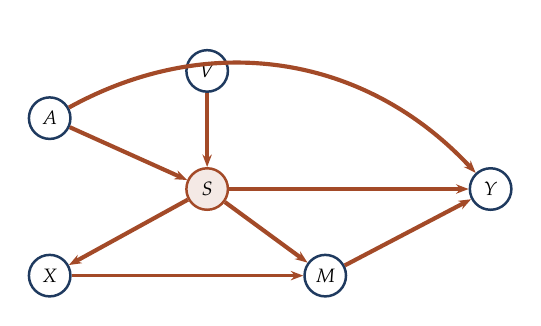
\begin{tikzpicture}[scale=1.0, every node/.style={font=\small}]
\node[knotenb] (a) at (-2.6,2.0) {$A$};
\node[knotenb] (v) at (-0.6,2.6) {$V$};
\node[knotenr] (s) at (-0.6,1.1) {$S$};
\node[knotenb] (x) at (-2.6,0.0) {$X$};
\node[knotenb] (m) at (0.9,0.0) {$M$};
\node[knotenb] (y) at (3.0,1.1) {$Y$};
\draw[kanted, -{Stealth[length=4.5pt]}] (a)--(s);
\draw[kanted, -{Stealth[length=4.5pt]}] (v)--(s);
\draw[kanted, -{Stealth[length=4.5pt]}] (s)--(x);
\draw[kanted, -{Stealth[length=4.5pt]}] (s)--(m);
\draw[akzent, line width=1.2pt, -{Stealth[length=4.5pt]}] (x)--(m);
\draw[kanted, -{Stealth[length=4.5pt]}] (m)--(y);
\draw[kanted, -{Stealth[length=4.5pt]}] (s)--(y);
\draw[kanted, -{Stealth[length=4.5pt]}] (a) to[bend left=38] (y);
\end{tikzpicture}
\end{center}

\begin{center}
\begin{minipage}{0.9\textwidth}
\textbf{Jeder Pfeil ist eine Annahme. Jeder \kursiv{fehlende} Pfeil ist auch eine --- und die schwerer wiegende.}
\end{minipage}
\end{center}

\begin{center}
\begin{minipage}{0.88\textwidth}
\kursiv{Dass kein Pfeil von $A$ nach $X$ führt, besagt: \textbf{Das Alter beeinflusst die Entscheidung über den Zeitpunkt nur über den Schweregrad} --- bei gleich schwer Kranken behandelt man Alte nicht anders als Junge. Das ist eine inhaltliche Behauptung, die man bestreiten kann und die man prüfen sollte. Ein Graph macht solche Behauptungen sichtbar; eine Regressionsgleichung versteckt sie.}
\end{minipage}
\end{center}
\end{merksatz}

\begin{definition}
\boxtitelm{Definition 4.1 --- kausaler Graph}
Ein \Begriff{kausaler Graph} ist ein gerichteter, kreisfreier Graph (Band 16, Kapitel~2), dessen Knoten die Größen sind. Ein Pfeil $U \to W$ bedeutet: $U$ ist eine \kursiv{unmittelbare} Ursache von $W$.

Dazu gehört ein \Begriff{strukturelles Gleichungsmodell}: Jede Größe wird durch ihre Elternknoten und eine eigene Zufallsgröße bestimmt,
\[ W = f_W\bigl(\text{Eltern}(W),\ \varepsilon_W\bigr) , \]
wobei die $\varepsilon$ voneinander unabhängig sind.
\end{definition}

\begin{merksatz}
\boxtitel{Satz 4.2 --- die Faktorisierung}
Erfüllt eine Verteilung ein solches Modell, so gilt
\[ \Pr[v_1,\ldots,v_k] = \prod_{i=1}^{k} \Pr\bigl[v_i \mid \text{Eltern}(v_i)\bigr] . \]

\schritt{Was das erspart}
\begin{center}
{\small
\renewcommand{\arraystretch}{1.48}
\begin{tabular}{@{}P{2.4cm}P{2.6cm}P{2.6cm}@{}}
\toprule
\textbf{Größen} & \textbf{volle Tabelle} & \textbf{Leitfall-Graph}\\
\midrule
$6$ & $63$ & $\mathbf{20}$\\
$10$ & $1023$ & \\
$20$ & $1\,048\,575$ & \\
\bottomrule
\end{tabular}}
\end{center}

\kursiv{Zur rechten Spalte:} $2^{0}+2^{0}+2^{2}+2^{1}+2^{2}+2^{3} = 1+1+4+2+4+8 = 20$.

\begin{center}
\begin{minipage}{0.88\textwidth}
\kursiv{\textbf{Die Ersparnis ist nicht der Zweck, sondern ein Nebengewinn.} Der Zweck ist, dass man die Annahmen einzeln hinschreiben und einzeln bestreiten kann. Aber die Ersparnis erklärt, warum sich solche Modelle auch dort durchgesetzt haben, wo es gar nicht um Ursachen geht --- in Band 22 etwa als Grundlage wahrscheinlichkeitstheoretischer Lernverfahren.}
\end{minipage}
\end{center}
\end{merksatz}

\section{Drei Bausteine}

\begin{merksatz}
\boxtitel{Jeder Weg besteht aus diesen drei}
\begin{center}
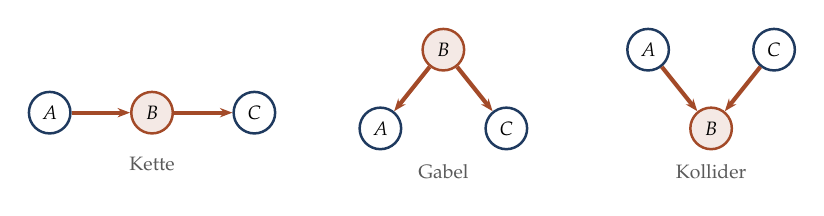
\begin{tikzpicture}[scale=1.0, every node/.style={font=\small}]
\node[knotenb] (a1) at (0,1.0) {$A$}; \node[knotenr] (b1) at (1.3,1.0) {$B$}; \node[knotenb] (c1) at (2.6,1.0) {$C$};
\draw[kanted, -{Stealth[length=4.5pt]}] (a1)--(b1); \draw[kanted, -{Stealth[length=4.5pt]}] (b1)--(c1);
\node[font=\scriptsize, color=grau] at (1.3,0.35) {Kette};

\node[knotenr] (b2) at (5.0,1.8) {$B$};
\node[knotenb] (a2) at (4.2,0.8) {$A$}; \node[knotenb] (c2) at (5.8,0.8) {$C$};
\draw[kanted, -{Stealth[length=4.5pt]}] (b2)--(a2); \draw[kanted, -{Stealth[length=4.5pt]}] (b2)--(c2);
\node[font=\scriptsize, color=grau] at (5.0,0.25) {Gabel};

\node[knotenb] (a3) at (7.6,1.8) {$A$}; \node[knotenb] (c3) at (9.2,1.8) {$C$};
\node[knotenr] (b3) at (8.4,0.8) {$B$};
\draw[kanted, -{Stealth[length=4.5pt]}] (a3)--(b3); \draw[kanted, -{Stealth[length=4.5pt]}] (c3)--(b3);
\node[font=\scriptsize, color=grau] at (8.4,0.25) {Kollider};
\end{tikzpicture}
\end{center}

\begin{center}
{\small
\renewcommand{\arraystretch}{1.55}
\begin{tabular}{@{}P{2.0cm}P{3.0cm}P{3.4cm}@{}}
\toprule
\textbf{Baustein} & \textbf{ohne Bedingung} & \textbf{gegeben $B$}\\
\midrule
Kette & $A$, $C$ abhängig & \textcolor{gruen}{unabhängig}\\
Gabel & $A$, $C$ abhängig & \textcolor{gruen}{unabhängig}\\
Kollider & \textcolor{gruen}{unabhängig} & \textcolor{akzent}{abhängig}\\
\bottomrule
\end{tabular}}
\end{center}

\begin{center}
\begin{minipage}{0.9\textwidth}
\textbf{Beim Kollider ist alles umgekehrt: Er sperrt von selbst und öffnet, sobald man auf ihn bedingt.}
\end{minipage}
\end{center}

\begin{center}
\begin{minipage}{0.88\textwidth}
\kursiv{Die dritte Zeile ist die Berkson-Verzerrung aus Aufgabe 1.2, nun als Baustein. \textbf{Und sie gilt auch, wenn man auf einen \kursiv{Nachkommen} des Kolliders bedingt} --- wer nach einem Merkmal auswählt, das vom Kollider abhängt, öffnet den Weg ebenfalls, wenn auch schwächer.}
\end{minipage}
\end{center}
\end{merksatz}

\begin{definition}
\boxtitelm{Definition 4.3 --- d-Trennung}
Ein Weg zwischen zwei Knoten heißt \Begriff{gesperrt} durch eine Menge $Z$, wenn er einen Knoten enthält, der
\begin{center}
{\small
\renewcommand{\arraystretch}{1.5}
\begin{tabular}{@{}P{1.0cm}P{7.4cm}@{}}
\toprule
$1$ & eine Kette oder Gabel bildet und in $Z$ liegt, \quad oder\\
$2$ & ein Kollider ist und weder selbst noch einer seiner Nachkommen in $Z$ liegt.\\
\bottomrule
\end{tabular}}
\end{center}
Zwei Knoten heißen \Begriff{d-getrennt} durch $Z$, wenn \kursiv{jeder} Weg zwischen ihnen gesperrt ist.
\end{definition}

\begin{merksatz}
\boxtitel{Satz 4.4 --- was d-Trennung bedeutet}
Sind $U$ und $W$ durch $Z$ d-getrennt, so sind sie in jeder Verteilung, die zum Graphen passt, bedingt unabhängig gegeben $Z$.

\begin{center}
\begin{minipage}{0.88\textwidth}
\kursiv{Der Beweis führt über die Faktorisierung aus Satz 4.2 und eine Induktion über die Wege; wir verzichten auf ihn --- die erste Auslassung dieses Bandes; die Fundstelle ist Pearl\zit{18}, Kapitel~1. \textbf{Die Umkehrung gilt \kursiv{fast} immer}: Sind zwei Knoten nicht d-getrennt, so sind sie für fast alle zum Graphen passenden Verteilungen abhängig --- Ausnahmen entstehen nur bei exakt sich aufhebenden Wirkungen.}
\end{minipage}
\end{center}

\begin{center}
\begin{minipage}{0.9\textwidth}
\textbf{Ein Bild wird damit zu einer Rechenvorschrift: Man liest Unabhängigkeiten ab, statt sie zu prüfen.}
\end{minipage}
\end{center}
\end{merksatz}

\section{Am Leitfall geprüft}

\begin{merksatz}
\boxtitel{Vier Fragen, abgelesen und nachgerechnet}
$400\,000$ erzeugte Patienten nach dem Modell aus Abschnitt 4.1:

\begin{center}
{\small
\renewcommand{\arraystretch}{1.5}
\begin{tabular}{@{}P{2.6cm}P{2.4cm}P{3.0cm}@{}}
\toprule
\textbf{Frage} & \textbf{Korrelation} & \textbf{abgelesen}\\
\midrule
$X$ und $A$ roh & $+0{,}188$ & abhängig über $S$\\
$X$ und $A$ gegeben $S$ & $-0{,}002$ & \textcolor{gruen}{d-getrennt}\\
$A$ und $V$ roh & $-0{,}001$ & \textcolor{gruen}{unabhängig}\\
$A$ und $V$ gegeben $S$ & $\mathbf{-0{,}107}$ & \textcolor{akzent}{Kollider geöffnet}\\
\bottomrule
\end{tabular}}
\end{center}

\schritt{Zur zweiten Zeile}
Es gibt zwei Wege von $X$ nach $A$:
\begin{center}
{\small
\renewcommand{\arraystretch}{1.48}
\begin{tabular}{@{}P{3.4cm}P{4.6cm}@{}}
\toprule
$X \leftarrow S \leftarrow A$ & Kette über $S$ --- durch $S$ gesperrt.\\
$X \leftarrow S \to M \to Y \leftarrow A$ & Kollider $Y$ --- von selbst gesperrt.\\
\bottomrule
\end{tabular}}
\end{center}
Beide gesperrt, also d-getrennt --- und die Korrelation fällt von $0{,}188$ auf $-0{,}002$. \checkmark

\schritt{Zur vierten Zeile}
$A$ und $V$ haben keine gemeinsame Ursache und keinen Pfeil zueinander --- sie sind unabhängig, und die Rechnung bestätigt es.

\begin{center}
\begin{minipage}{0.9\textwidth}
\textbf{Bedingt man auf den Schweregrad, so wird aus Unabhängigkeit eine Korrelation von $-0{,}107$.}
\end{minipage}
\end{center}

\begin{center}
\begin{minipage}{0.88\textwidth}
\kursiv{$S$ ist ein Kollider von $A$ und $V$. \textbf{Unter den Schwerkranken erklärt das hohe Alter den Schweregrad --- also braucht es die Vorerkrankungen nicht mehr}, und umgekehrt. Wer den Schweregrad \enquote{herausrechnet}, erzeugt damit einen Zusammenhang zwischen Alter und Vorerkrankungen, den es in der Bevölkerung nicht gibt. Kapitel~5 zeigt, wann das schadet.}
\end{minipage}
\end{center}
\end{merksatz}

\section{Der Bruchfall}

\begin{warnung}
\boxtitelr{Der Graph ist nicht in den Daten}
\begin{center}
{\small
\renewcommand{\arraystretch}{1.52}
\begin{tabular}{@{}P{2.8cm}P{5.8cm}@{}}
\toprule
\textbf{Gleiche Muster} & Mehrere Graphen erzeugen genau dieselben Unabhängigkeiten. Die Daten können zwischen ihnen nicht entscheiden.\\
\textbf{Verborgene Größen} & Was nicht gemessen ist, fehlt im Graphen --- und verändert alle Schlüsse.\\
\textbf{Kreise} & Rückkopplungen --- Fieber erhöht Herzfrequenz erhöht Fieber --- sind in einem kreisfreien Graphen nicht darstellbar.\\
\bottomrule
\end{tabular}}
\end{center}

\schritt{Zur ersten Zeile}
\begin{center}
{\small
\renewcommand{\arraystretch}{1.5}
\begin{tabular}{@{}P{3.0cm}P{2.6cm}P{2.6cm}@{}}
\toprule
\textbf{Graph} & $X \perp Y$? & $X \perp Y \mid S$?\\
\midrule
$X \to S \to Y$ & nein & \textcolor{gruen}{ja}\\
$X \leftarrow S \leftarrow Y$ & nein & \textcolor{gruen}{ja}\\
$X \leftarrow S \to Y$ & nein & \textcolor{gruen}{ja}\\
\midrule
$X \to S \leftarrow Y$ & \textcolor{gruen}{ja} & nein\\
\bottomrule
\end{tabular}}
\end{center}

\begin{center}
\begin{minipage}{0.9\textwidth}
\textbf{Die ersten drei sind an den Daten nicht zu unterscheiden --- der vierte schon.}
\end{minipage}
\end{center}

\begin{center}
\begin{minipage}{0.88\textwidth}
\kursiv{\textbf{Das ist Satz 1.2 in grafischer Gestalt.} Die Daten legen das Gerüst fest --- welche Knoten verbunden sind --- und die Kollider; die übrigen Pfeilrichtungen nicht. Man nennt die Menge der ununterscheidbaren Graphen eine \Begriff{Markow-Äquivalenzklasse}. Immerhin sind Kollider erkennbar, und das ist mehr, als Kapitel~1 vermuten ließ; Abschnitt 4.5 des Forschungskastens nutzt es aus.}
\end{minipage}
\end{center}

\schritt{Zur zweiten Zeile}
\begin{center}
\begin{minipage}{0.88\textwidth}
\kursiv{Nimmt man im Leitfall eine unbeobachtete Größe an --- etwa die Erfahrung des diensthabenden Arztes, die sowohl den Zeitpunkt als auch die weitere Behandlung beeinflusst ---, so entsteht ein zusätzlicher Weg von $X$ nach $Y$, den keine Anpassung an $S$ sperrt. \textbf{Man zeichnet solche Größen als gestrichelte Doppelpfeile ein}, und Kapitel~6 sagt, wann sie schaden und wann nicht.}
\end{minipage}
\end{center}
\end{warnung}

\section{Übungsaufgaben}

\begin{aufgabe}
\boxtitel{Aufgabe 4.1 --- Wege sperren}
Im Graphen des Leitfalls: Welche der folgenden Aussagen gelten?
\begin{center}
{\small
\renewcommand{\arraystretch}{1.5}
\begin{tabular}{@{}P{1.0cm}P{7.4cm}@{}}
\toprule
(a) & $V \perp Y \mid S$\\
(b) & $X \perp Y \mid S$\\
(c) & $X \perp A \mid S, M$\\
\bottomrule
\end{tabular}}
\end{center}

\loesung
\schritt{(a) --- Wege von $V$ nach $Y$}
\begin{center}
{\small
\renewcommand{\arraystretch}{1.46}
\begin{tabular}{@{}P{3.6cm}P{4.4cm}@{}}
\toprule
\textbf{Weg} & \textbf{gegeben $S$}\\
\midrule
$V \to S \to Y$ & Kette, gesperrt\\
$V \to S \to M \to Y$ & Kette, gesperrt\\
$V \to S \to X \to M \to Y$ & Kette, gesperrt\\
$V \to S \leftarrow A \to Y$ & $S$ ist Kollider, \textcolor{akzent}{geöffnet}\\
\bottomrule
\end{tabular}}
\end{center}

\begin{center}
\begin{minipage}{0.9\textwidth}
\textbf{(a) gilt nicht.} Der letzte Weg wird durch das Bedingen auf $S$ gerade geöffnet.
\end{minipage}
\end{center}

\kursiv{Inhaltlich:} Unter Schwerkranken sind die ohne Vorerkrankungen eher die Alten --- und Alter erhöht die Sterblichkeit unmittelbar. So entsteht ein Zusammenhang zwischen $V$ und $Y$.

\schritt{(b) --- Wege von $X$ nach $Y$}
\begin{center}
{\small
\renewcommand{\arraystretch}{1.46}
\begin{tabular}{@{}P{3.6cm}P{4.4cm}@{}}
\toprule
\textbf{Weg} & \textbf{gegeben $S$}\\
\midrule
$X \to M \to Y$ & \textcolor{akzent}{offen} --- das ist die Wirkung\\
$X \leftarrow S \to Y$ & gesperrt\\
$X \leftarrow S \to M \to Y$ & gesperrt\\
\bottomrule
\end{tabular}}
\end{center}

\begin{center}
\begin{minipage}{0.9\textwidth}
\textbf{(b) gilt nicht --- und soll es auch nicht.} Der offene Weg ist der ursächliche; genau ihn will man messen.
\end{minipage}
\end{center}

\kursiv{Die Rechnung ergab $-0{,}021$} --- klein, aber von null verschieden: die Schutzwirkung der frühen Gabe.

\schritt{(c) --- mit $M$ im Bedingungssatz}
\begin{center}
{\small
\renewcommand{\arraystretch}{1.46}
\begin{tabular}{@{}P{3.8cm}P{4.2cm}@{}}
\toprule
\textbf{Weg} & \textbf{gegeben $S$ und $M$}\\
\midrule
$X \leftarrow S \leftarrow A$ & gesperrt durch $S$\\
$X \to M \leftarrow S \to \ldots$ & --- \\
$X \to M \to Y \leftarrow A$ & $M$ in $Z$: offen; $Y$ Kollider: gesperrt\\
\bottomrule
\end{tabular}}
\end{center}

\begin{center}
\begin{minipage}{0.9\textwidth}
\textbf{(c) gilt.} Alle Wege bleiben gesperrt.
\end{minipage}
\end{center}

\begin{center}
\begin{minipage}{0.88\textwidth}
\kursiv{Hier ist das Bedingen auf $M$ unschädlich für diese Frage --- \textbf{aber es wäre schädlich für die Schätzung des Effekts von $X$ auf $Y$}, weil es den ursächlichen Weg $X \to M \to Y$ durchschneidet. Dieselbe Größe kann für die eine Frage harmlos und für die andere verheerend sein. Kapitel~5 macht daraus eine Systematik.}
\end{minipage}
\end{center}
\end{aufgabe}

\begin{aufgabe}
\boxtitel{Aufgabe 4.2 --- Wie viele Zahlen}
Wie viele Wahrscheinlichkeiten braucht man für die gemeinsame Verteilung von zehn binären Größen --- ohne Graph, und mit einem Graphen, in dem jede Größe höchstens drei Eltern hat?

\loesung
\schritt{Schritt 1 --- Ohne Graph}
\[ 2^{10} - 1 = 1023 \]

\schritt{Schritt 2 --- Mit Graph}
Je Größe braucht man eine Wahrscheinlichkeit für jede Belegung der Eltern:
\[ \sum_{i=1}^{10} 2^{|\text{Eltern}(i)|} \ \le\ 10\cdot2^{3} = 80 \]

\begin{center}
{\small
\renewcommand{\arraystretch}{1.48}
\begin{tabular}{@{}P{2.4cm}P{2.4cm}P{2.4cm}@{}}
\toprule
\textbf{Größen} & \textbf{ohne Graph} & \textbf{höchstens $3$ Eltern}\\
\midrule
$10$ & $1023$ & $\le 80$\\
$20$ & $\approx 10^{6}$ & $\le 160$\\
$50$ & $\approx 10^{15}$ & $\le 400$\\
\bottomrule
\end{tabular}}
\end{center}

\schritt{Schritt 3 --- Die Bedeutung}
\begin{center}
\begin{minipage}{0.88\textwidth}
\kursiv{Die volle Tabelle wächst exponentiell, das Modell linear. \textbf{Bei fünfzig Größen bräuchte man mehr Patienten, als es Menschen gibt} --- mit Graph genügen einige tausend. Das ist derselbe Gewinn wie in Band 22, Kapitel~10: Eine Annahme über die Struktur macht aus einer unmöglichen Aufgabe eine lösbare.}
\end{minipage}
\end{center}

\schritt{Schritt 4 --- Der Preis}
\begin{center}
\begin{minipage}{0.88\textwidth}
\kursiv{Man bezahlt mit der Richtigkeit der Struktur. \textbf{Fehlt ein Pfeil, den es gibt, so ist das Modell falsch --- und zwar ohne dass ein Rechenverfahren das bemerkte.} Zu viele Pfeile schaden dagegen nur der Genauigkeit, nicht der Gültigkeit. Im Zweifel zeichnet man den Pfeil ein.}
\end{minipage}
\end{center}
\end{aufgabe}

\begin{aufgabe}
\boxtitel{Aufgabe 4.3 --- Was die Daten verraten}
Man beobachte an drei Größen: $X$ und $Y$ sind abhängig, $X$ und $S$ sind abhängig, $S$ und $Y$ sind abhängig --- aber $X \perp Y \mid S$. Welche Graphen kommen in Frage?

\loesung
\schritt{Schritt 1 --- Das Gerüst}
Alle drei Paare hängen zusammen, aber $X$ und $Y$ werden durch $S$ getrennt. Also gibt es keinen Pfeil zwischen $X$ und $Y$:
\[ X - S - Y \]

\schritt{Schritt 2 --- Die möglichen Richtungen}
\begin{center}
{\small
\renewcommand{\arraystretch}{1.48}
\begin{tabular}{@{}P{3.0cm}P{2.4cm}P{2.6cm}@{}}
\toprule
\textbf{Graph} & \textbf{Art} & $X \perp Y \mid S$?\\
\midrule
$X \to S \to Y$ & Kette & \textcolor{gruen}{ja}\\
$X \leftarrow S \leftarrow Y$ & Kette & \textcolor{gruen}{ja}\\
$X \leftarrow S \to Y$ & Gabel & \textcolor{gruen}{ja}\\
$X \to S \leftarrow Y$ & Kollider & nein\\
\bottomrule
\end{tabular}}
\end{center}

\begin{center}
\begin{minipage}{0.9\textwidth}
\textbf{Drei Graphen bleiben übrig. Der Kollider ist ausgeschlossen.}
\end{minipage}
\end{center}

\schritt{Schritt 3 --- Was das praktisch heißt}
\begin{center}
{\small
\renewcommand{\arraystretch}{1.5}
\begin{tabular}{@{}P{2.8cm}P{5.8cm}@{}}
\toprule
\textbf{Kette} & $X$ wirkt auf $Y$ --- über $S$. Eingriff in $X$ hilft.\\
\textbf{Gabel} & $S$ verursacht beides. Eingriff in $X$ hilft nicht.\\
\bottomrule
\end{tabular}}
\end{center}

\begin{center}
\begin{minipage}{0.88\textwidth}
\kursiv{\textbf{Die Daten entscheiden nicht, ob ein Eingriff hilft} --- genau wie in Satz 1.2. Was sie entscheiden, ist eine Teilfrage: Sie schließen den Kollider aus. Und manchmal genügt Wissen über die Zeit: Liegt $X$ zeitlich vor $S$, so sind die letzten beiden Zeilen ausgeschlossen, und es bleibt die Kette.}
\end{minipage}
\end{center}

\schritt{Schritt 4 --- Im Leitfall}
\begin{center}
\begin{minipage}{0.88\textwidth}
\kursiv{Dort ist die Richtung klar: Der Schweregrad besteht bei Aufnahme, die Gabe erfolgt danach. \textbf{Die Zeitordnung ist die wichtigste Quelle kausalen Wissens} --- und der Grund, warum man bei jeder Größe festhalten sollte, wann sie erhoben wurde. Das war bereits die Lehre aus Band 22, Kapitel~3, wo ein Merkmal aus der Zukunft das Modell verdarb.}
\end{minipage}
\end{center}
\end{aufgabe}

\begin{geschichte}
\boxtitelg{Von den Pfadkoeffizienten zu den Graphen}
\Person{Sewall Wright} (1889--1988) führte 1918 die Pfadanalyse ein --- für die Vererbung der Fellzeichnung bei Meerschweinchen.

\begin{center}
\begin{minipage}{0.9\textwidth}
\kursiv{Er zeichnete gerichtete Diagramme und gab Regeln an, wie sich Korrelationen aus den Pfadkoeffizienten zusammensetzen. \textbf{Die Statistik seiner Zeit lehnte das ab}: Wrights Lehrer \Person{Karl Pearson} und später \Person{Ronald Fisher} hielten Kausalaussagen aus Beobachtungsdaten für unwissenschaftlich. Wrights Verfahren überlebte in der Genetik und in der Soziologie, nicht in der Statistik.}
\end{minipage}
\end{center}

\schritt{Pearl}
\Person{Judea Pearl} entwickelte in den 1980er Jahren Bayessche Netze für die künstliche Intelligenz --- zunächst ohne kausale Deutung, als Werkzeug zum effizienten Rechnen mit Wahrscheinlichkeiten.

\begin{center}
\begin{minipage}{0.9\textwidth}
\kursiv{Die d-Trennung stammt aus dieser Arbeit. \textbf{Erst um 1990 zog er die Folgerung, dass dieselben Graphen Ursachen darstellen können}, wenn man die Pfeile ernst nimmt und den Eingriff als Durchtrennen deutet. Sein Buch \kursiv{Causality} von 2000 machte daraus ein geschlossenes Gebäude; 2011 erhielt er den Turing-Preis.}
\end{minipage}
\end{center}

\schritt{Zwei Schulen}
\begin{center}
\begin{minipage}{0.9\textwidth}
\kursiv{Die Sprache der potentiellen Ergebnisse aus Kapitel~2 und die der Graphen entstanden getrennt und standen sich lange feindlich gegenüber. \textbf{Sie sind nachweislich gleichwertig} --- jede Aussage der einen lässt sich in die andere übersetzen ---, und heute benutzt man beide nebeneinander: Graphen, um die Annahmen zu finden, potentielle Ergebnisse, um die Schätzer aufzuschreiben. Dieser Band verfährt ebenso.}
\end{minipage}
\end{center}
\end{geschichte}

\begin{forschung}
\boxtitelp{Graphen heute}
\begin{center}
{\small
\renewcommand{\arraystretch}{1.45}
\begin{tabular}{@{}P{2.8cm}P{5.4cm}@{}}
\toprule
\textbf{Struktur lernen} & Aus Daten die Äquivalenzklasse bestimmen --- nicht mehr, aber auch nicht weniger.\\
\textbf{Mit Eingriffen} & Wenige gezielte Versuche genügen, um die Richtungen festzulegen.\\
\textbf{Große Graphen} & Genregulation mit Tausenden von Knoten.\\
\bottomrule
\end{tabular}}
\end{center}

\schritt{Zur zweiten Zeile}
\begin{center}
\begin{minipage}{0.88\textwidth}
\kursiv{Kann man einzelne Größen gezielt verändern --- in der Zellbiologie etwa durch Ausschalten eines Gens ---, so lassen sich Richtungen bestimmen, die aus Beobachtung allein nicht folgen. \textbf{Die Zahl der nötigen Eingriffe wächst dabei nur logarithmisch mit der Knotenzahl}, wenn man sie geschickt wählt. Das ist eines der wenigen Ergebnisse, bei denen Theorie und Laborpraxis sich unmittelbar treffen.}
\end{minipage}
\end{center}
\end{forschung}

\begin{merksatz}
\boxtitel{Was Sie jetzt können}
\begin{center}
\renewcommand{\arraystretch}{1.5}
\begin{tabular}{@{}P{3.0cm}P{5.6cm}@{}}
\toprule
\textbf{Definition 4.1} & Pfeile sind Annahmen, fehlende auch\\
\textbf{Satz 4.2} & Faktorisierung über die Eltern\\
\textbf{Drei Bausteine} & Kette, Gabel, Kollider\\
\textbf{Definition 4.3} & d-Trennung: alle Wege gesperrt\\
\textbf{Satz 4.4} & d-getrennt heißt bedingt unabhängig\\
\bottomrule
\end{tabular}
\end{center}

\begin{center}
\begin{minipage}{0.88\textwidth}
\kursiv{Man kann nun Annahmen aufschreiben und Unabhängigkeiten ablesen. Das nächste Kapitel beantwortet die praktische Frage, die daraus folgt: Welche Größen soll man herausrechnen --- und welche auf keinen Fall?}
\end{minipage}
\end{center}
\end{merksatz}

\chapter{Was man herausrechnen darf}

\section{Die Frage}

\begin{merksatz}
\boxtitel{Sechs Größen, welche ins Modell?}
Im Leitfall stehen Alter, Vorerkrankungen, Schweregrad, Organversagen und die Behandlung zur Verfügung. Die übliche Antwort lautet: möglichst alle --- je mehr man berücksichtigt, desto besser.

\begin{center}
\begin{minipage}{0.9\textwidth}
\textbf{Diese Antwort ist falsch, und zwar nicht nur ungenau, sondern im Vorzeichen.}
\end{minipage}
\end{center}

\begin{center}
\begin{minipage}{0.88\textwidth}
\kursiv{Dieses Kapitel unterscheidet vier Rollen, die eine Größe im Graphen spielen kann. \textbf{Bei zweien muss man anpassen, bei zweien darf man es auf keinen Fall} --- und welche Rolle vorliegt, steht nicht in den Daten, sondern im Graphen aus Kapitel~4.}
\end{minipage}
\end{center}
\end{merksatz}

\section{Vier Rollen}

\begin{merksatz}
\boxtitel{Die Übersicht}
\begin{center}
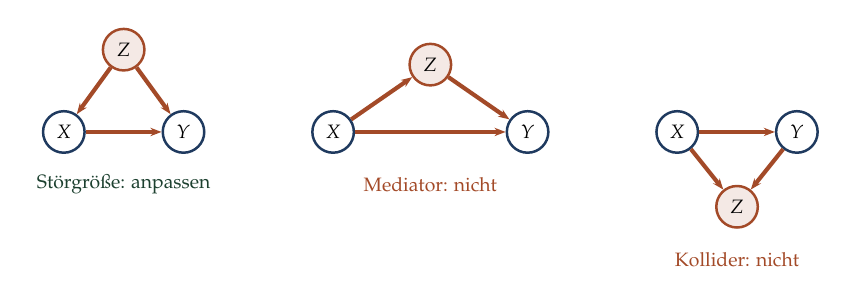
\begin{tikzpicture}[scale=0.95, every node/.style={font=\scriptsize}]
% Störgröße
\node[knotenr] (z1) at (0.8,1.6) {$Z$};
\node[knotenb] (x1) at (0,0.5) {$X$}; \node[knotenb] (y1) at (1.6,0.5) {$Y$};
\draw[kanted, -{Stealth[length=4pt]}] (z1)--(x1); \draw[kanted, -{Stealth[length=4pt]}] (z1)--(y1);
\draw[kanted, -{Stealth[length=4pt]}] (x1)--(y1);
\node[color=gruen!60!black] at (0.8,-0.2) {Störgröße: anpassen};
% Mediator
\node[knotenb] (x2) at (3.6,0.5) {$X$}; \node[knotenr] (z2) at (4.9,1.4) {$Z$}; \node[knotenb] (y2) at (6.2,0.5) {$Y$};
\draw[kanted, -{Stealth[length=4pt]}] (x2)--(z2); \draw[kanted, -{Stealth[length=4pt]}] (z2)--(y2);
\draw[kanted, -{Stealth[length=4pt]}] (x2)--(y2);
\node[color=akzent] at (4.9,-0.2) {Mediator: nicht};
% Kollider
\node[knotenb] (x3) at (8.2,0.5) {$X$}; \node[knotenb] (y3) at (9.8,0.5) {$Y$};
\node[knotenr] (z3) at (9.0,-0.5) {$Z$};
\draw[kanted, -{Stealth[length=4pt]}] (x3)--(z3); \draw[kanted, -{Stealth[length=4pt]}] (y3)--(z3);
\draw[kanted, -{Stealth[length=4pt]}] (x3)--(y3);
\node[color=akzent] at (9.0,-1.2) {Kollider: nicht};
\end{tikzpicture}
\end{center}

\begin{center}
{\small
\renewcommand{\arraystretch}{1.55}
\begin{tabular}{@{}P{2.2cm}P{3.2cm}P{3.2cm}@{}}
\toprule
\textbf{Rolle} & \textbf{Lage im Graphen} & \textbf{anpassen?}\\
\midrule
Störgröße & Ursache von $X$ und von $Y$ & \textcolor{gruen}{ja --- muss}\\
Mediator & liegt auf dem Weg $X \to Y$ & \textcolor{akzent}{nein}\\
Kollider & Folge von $X$ und von $Y$ & \textcolor{akzent}{nein}\\
Instrument & Ursache nur von $X$ & \textcolor{akzent}{nein}\\
\bottomrule
\end{tabular}}
\end{center}

\begin{center}
\begin{minipage}{0.9\textwidth}
\textbf{Nur die erste Zeile rechtfertigt die Anpassung. Die übrigen drei schaden --- jede auf eigene Weise.}
\end{minipage}
\end{center}
\end{merksatz}

\section{Was in jedem Fall geschieht}

\begin{merksatz}
\boxtitel{Alle vier durchgerechnet}
Jeweils $200\,000$ erzeugte Patienten, lineare Modelle, geschätzt durch kleinste Quadrate.

\schritt{Erstens --- der Mediator}
$X$ wirkt \kursiv{nur} über $M$ auf $Y$; wahrer Gesamteffekt $0{,}8\cdot0{,}9 = 0{,}72$. Eine Störgröße $U$ ist beobachtet.

\begin{center}
{\small
\renewcommand{\arraystretch}{1.48}
\begin{tabular}{@{}P{3.0cm}P{2.2cm}P{2.6cm}@{}}
\toprule
\textbf{Modell} & \textbf{Schätzung} & \\
\midrule
$Y \sim X$ & $1{,}217$ & verzerrt durch $U$\\
$Y \sim X + U$ & $\mathbf{0{,}720}$ & \textcolor{gruen}{richtig}\\
$Y \sim X + M + U$ & $\mathbf{0{,}004}$ & \textcolor{akzent}{Effekt verschwunden}\\
\bottomrule
\end{tabular}}
\end{center}

\begin{center}
\begin{minipage}{0.88\textwidth}
\kursiv{\textbf{Wer den Mediator anpasst, misst den Effekt \kursiv{bei festgehaltenem} Organversagen} --- und der ist null, weil die Behandlung nur über das Organversagen wirkt. Das Ergebnis ist rechnerisch richtig und beantwortet die falsche Frage. Kapitel~13 behandelt die Fälle, in denen man genau das absichtlich tut.}
\end{minipage}
\end{center}

\schritt{Zweitens --- der Kollider}
$A$ und $B$ sind unabhängig; beide verursachen $S$.

\begin{center}
{\small
\renewcommand{\arraystretch}{1.48}
\begin{tabular}{@{}P{2.6cm}P{2.4cm}P{2.6cm}@{}}
\toprule
\textbf{Modell} & \textbf{Koeffizient} & \\
\midrule
$A \sim B$ & $0{,}002$ & \textcolor{gruen}{unabhängig}\\
$A \sim B + S$ & $\mathbf{-0{,}390}$ & \textcolor{akzent}{erfunden}\\
\bottomrule
\end{tabular}}
\end{center}

\begin{center}
\begin{minipage}{0.88\textwidth}
\kursiv{Aus nichts wird ein deutlicher negativer Zusammenhang. \textbf{Das ist die Berkson-Verzerrung aus Aufgabe 1.2 --- nur nicht durch Auswahl, sondern durch Anpassung erzeugt.} Für die Verzerrung ist es gleichgültig, ob man nur Aufgenommene betrachtet oder die Aufnahme als Kovariable ins Modell nimmt.}
\end{minipage}
\end{center}

\schritt{Drittens --- das Instrument}
$Z$ wirkt nur auf $X$; eine \kursiv{unbeobachtete} Störgröße $U$ bleibt im Modell fehlen.

\begin{center}
{\small
\renewcommand{\arraystretch}{1.48}
\begin{tabular}{@{}P{2.6cm}P{2.2cm}P{2.6cm}@{}}
\toprule
\textbf{Modell} & \textbf{Schätzung} & \textbf{Verzerrung}\\
\midrule
$Y \sim X$ & $1{,}186$ & $+0{,}186$\\
$Y \sim X + Z$ & $1{,}403$ & $\mathbf{+0{,}403}$\\
\bottomrule
\end{tabular}}
\end{center}

\begin{center}
\begin{minipage}{0.9\textwidth}
\textbf{Die Anpassung an das Instrument verdoppelt die Verzerrung.}
\end{minipage}
\end{center}

\begin{center}
\begin{minipage}{0.88\textwidth}
\kursiv{Der Grund: $Z$ erklärt einen Teil der Schwankung von $X$, der \kursiv{nicht} von $U$ stammt. Was von $X$ übrig bleibt, ist stärker von $U$ durchsetzt --- und damit wiegt die verbliebene Verzerrung schwerer. \textbf{Man nennt das Verstärkungsverzerrung}, und sie ist besonders tückisch, weil das Modell mit $Z$ genauer aussieht: Es erklärt mehr Streuung und hat engere Vertrauensintervalle.}
\end{minipage}
\end{center}
\end{merksatz}

\begin{warnung}
\boxtitelr{Viertens --- eine Größe, die gar nichts damit zu tun hat}
$W$ ist weder Ursache von $X$ noch von $Y$. Sie ist Kollider zweier unbeobachteter Größen: $U_1$ wirkt auf $X$ und auf $W$, $U_3$ wirkt auf $W$ und auf $Y$.

\begin{center}
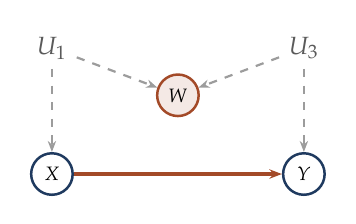
\begin{tikzpicture}[scale=1.0, every node/.style={font=\small}]
\node[grau, font=\small] (u1) at (-1.6,1.6) {$U_1$};
\node[grau, font=\small] (u3) at (1.6,1.6) {$U_3$};
\node[knotenr] (w) at (0,1.0) {$W$};
\node[knotenb] (x) at (-1.6,0.0) {$X$};
\node[knotenb] (y) at (1.6,0.0) {$Y$};
\draw[grau!60, line width=0.8pt, dashed, -{Stealth[length=4pt]}] (u1)--(w);
\draw[grau!60, line width=0.8pt, dashed, -{Stealth[length=4pt]}] (u3)--(w);
\draw[grau!60, line width=0.8pt, dashed, -{Stealth[length=4pt]}] (u1)--(x);
\draw[grau!60, line width=0.8pt, dashed, -{Stealth[length=4pt]}] (u3)--(y);
\draw[kanted, -{Stealth[length=4.5pt]}] (x)--(y);
\end{tikzpicture}
\end{center}

\begin{center}
{\small
\renewcommand{\arraystretch}{1.48}
\begin{tabular}{@{}P{2.6cm}P{2.2cm}P{2.6cm}@{}}
\toprule
\textbf{Modell} & \textbf{Schätzung} & \textbf{wahr: $1{,}000$}\\
\midrule
$Y \sim X$ & $\mathbf{0{,}999}$ & \textcolor{gruen}{unverzerrt}\\
$Y \sim X + W$ & $\mathbf{0{,}863}$ & \textcolor{akzent}{verzerrt}\\
\bottomrule
\end{tabular}}
\end{center}

\begin{center}
\begin{minipage}{0.9\textwidth}
\textbf{Ohne Anpassung richtig, mit Anpassung falsch --- und $W$ liegt zeitlich vor der Behandlung.}
\end{minipage}
\end{center}

\begin{center}
\begin{minipage}{0.88\textwidth}
\kursiv{Man nennt das nach der Form des Graphen die \Begriff{M-Verzerrung}. \textbf{Sie widerlegt die verbreitete Regel, man dürfe gefahrlos alles anpassen, was vor der Behandlung erhoben wurde.} Ohne Graph ist $W$ von einer echten Störgröße nicht zu unterscheiden: Beide hängen mit $X$ und mit $Y$ zusammen.}
\end{minipage}
\end{center}
\end{warnung}

\section{Der Fehler der zweiten Tabelle}

\begin{merksatz}
\boxtitel{Koeffizienten sind nicht alle gleich zu lesen}
Eine übliche Veröffentlichung zeigt in der zweiten Tabelle ein Modell mit allen Kovariablen und deutet jeden Koeffizienten als Wirkung.

\begin{center}
{\small
\renewcommand{\arraystretch}{1.5}
\begin{tabular}{@{}P{3.0cm}P{5.6cm}@{}}
\toprule
\textbf{Die Behandlung} & Ihr Koeffizient ist kausal deutbar --- wenn der Satz aus Kapitel~6 erfüllt ist.\\
\textbf{Die Kovariablen} & Ihre Koeffizienten sind es in aller Regel \textcolor{akzent}{nicht}.\\
\bottomrule
\end{tabular}}
\end{center}

\begin{center}
\begin{minipage}{0.88\textwidth}
\kursiv{Die Anpassungsmenge wurde gewählt, um die Wege um \kursiv{die Behandlung} zu sperren --- nicht die um das Alter. \textbf{Für das Alter kann dieselbe Menge zu wenig enthalten (eine Störgröße fehlt) oder zu viel (ein Mediator ist dabei).} Im Leitfall ist der Schweregrad ein Mediator zwischen Alter und Tod: Der Alterskoeffizient misst dann nur den direkten Anteil und unterschätzt die Gesamtwirkung des Alters.}
\end{minipage}
\end{center}

\begin{center}
\begin{minipage}{0.9\textwidth}
\textbf{Ein Modell, ein deutbarer Koeffizient.} Wer mehrere Wirkungen wissen will, braucht mehrere Modelle mit jeweils eigener Anpassungsmenge.
\end{minipage}
\end{center}
\end{merksatz}

\section{Der Bruchfall}

\begin{warnung}
\boxtitelr{Wenn die Störgröße ungenau gemessen ist}
Passt man an eine fehlerhaft gemessene Störgröße an, so bleibt ein Teil der Verzerrung bestehen.

\begin{center}
{\small
\renewcommand{\arraystretch}{1.52}
\begin{tabular}{@{}P{2.8cm}P{5.8cm}@{}}
\toprule
\textbf{Restverzerrung} & Der Schweregrad in zwei Stufen ist ein grobes Abbild einer stetigen Größe. Was innerhalb der Stufen schwankt, bleibt unkorrigiert.\\
\textbf{Stellvertreter} & Ein gemessener Wert ersetzt oft eine nicht messbare Größe --- etwa die Laborwerte den \enquote{Zustand}. Die Anpassung ist dann unvollständig.\\
\bottomrule
\end{tabular}}
\end{center}

\begin{center}
\begin{minipage}{0.88\textwidth}
\kursiv{\textbf{Eine Anpassung an einen Stellvertreter beseitigt die Verzerrung nur teilweise}, und wie viel übrig bleibt, hängt davon ab, wie gut der Stellvertreter ist. In der Praxis ist das die häufigste Ursache dafür, dass Beobachtungsstudien und randomisierte Studien auseinanderfallen. Kapitel~11 behandelt Verfahren, die diesen Rest abschätzen.}
\end{minipage}
\end{center}

\schritt{Und eine Ausnahme von der Regel}
\begin{center}
\begin{minipage}{0.88\textwidth}
\kursiv{Nicht jede Anpassung an einen Nicht-Störfaktor schadet. \textbf{Eine Größe, die nur auf $Y$ wirkt und nicht auf $X$, darf man anpassen} --- sie verzerrt nicht und verringert sogar die Streuung, genau wie in der randomisierten Studie aus Kapitel~3. Die vier Rollen sind also nicht vollständig; die allgemeine Regel liefert erst der Hintertürtest des nächsten Kapitels.}
\end{minipage}
\end{center}
\end{warnung}

\section{Übungsaufgaben}

\begin{aufgabe}
\boxtitel{Aufgabe 5.1 --- Den Mediator erkennen}
Im Leitfall soll der Effekt der frühen Gabe auf den Tod geschätzt werden. Welche der fünf übrigen Größen gehören ins Modell?

\loesung
\schritt{Schritt 1 --- Die Rollen bestimmen}
\begin{center}
{\small
\renewcommand{\arraystretch}{1.5}
\begin{tabular}{@{}P{2.4cm}P{3.0cm}P{2.6cm}@{}}
\toprule
\textbf{Größe} & \textbf{Rolle} & \textbf{anpassen?}\\
\midrule
$S$ Schweregrad & Ursache von $X$ und $Y$ & \textcolor{gruen}{ja}\\
$A$ Alter & Ursache von $S$ und $Y$ & \textcolor{gruen}{darf}\\
$V$ Vorerkrankungen & Ursache nur von $S$ & \textcolor{akzent}{nein}\\
$M$ Organversagen & Mediator & \textcolor{akzent}{nein}\\
\bottomrule
\end{tabular}}
\end{center}

\schritt{Schritt 2 --- Die drei Begründungen}
\kursiv{$S$:} Er liegt auf dem Weg $X \leftarrow S \to Y$. Ohne Anpassung bleibt dieser offen --- das war Kapitel~1.

\kursiv{$A$:} Das Alter wirkt auf $Y$ unmittelbar und auf $X$ nur über $S$. Passt man ohnehin an $S$ an, so ist $A$ nicht nötig --- aber unschädlich und streuungsmindernd.

\kursiv{$V$:} Die Vorerkrankungen wirken nur über $S$. Sie sind ein \kursiv{Instrument} für $X$ --- und nach Abschnitt 5.3 kann ihre Anpassung eine verbliebene Verzerrung verstärken.

\kursiv{$M$:} Mediator. Seine Anpassung setzt den Effekt auf null.

\schritt{Schritt 3 --- Die Antwort}
\begin{center}
\begin{minipage}{0.9\textwidth}
\textbf{Es genügt $\{S\}$, und $\{S, A\}$ ist ebenso richtig. $V$ und $M$ gehören nicht hinein.}
\end{minipage}
\end{center}

\schritt{Schritt 4 --- Was ein Rechner nicht sieht}
\begin{center}
\begin{minipage}{0.88\textwidth}
\kursiv{Nimmt man alle fünf Größen ins Modell --- wie es viele Auswertungsprogramme vorschlagen ---, so ist das Ergebnis falsch, und zwar dreifach: \textbf{Der Mediator tilgt den Effekt, das Instrument verstärkt die Restverzerrung, und die Alterskoeffizienten verleiten zum Fehler der zweiten Tabelle.} Nichts davon zeigt sich in den Gütemaßen: Das volle Modell erklärt mehr Streuung als das richtige.}
\end{minipage}
\end{center}
\end{aufgabe}

\begin{aufgabe}
\boxtitel{Aufgabe 5.2 --- Den Kollider in Zahlen}
Alter und Vorerkrankungen sind in der Bevölkerung unabhängig. Beide erhöhen den Schweregrad. Nach Kapitel~4 beträgt ihre Korrelation unter Festhalten des Schweregrads $-0{,}107$. Was folgt daraus für eine Studie an Schwerkranken?

\loesung
\schritt{Schritt 1 --- Die Lage}
Eine Studie, die nur Schwerkranke einschließt, hat auf $S$ bedingt --- nicht durch Rechnung, sondern durch die Einschlusskriterien.

\schritt{Schritt 2 --- Die Folge}
\begin{center}
{\small
\renewcommand{\arraystretch}{1.48}
\begin{tabular}{@{}P{2.8cm}P{2.6cm}@{}}
\toprule
\textbf{Bevölkerung} & $r = -0{,}001$\\
\textbf{nur Schwerkranke} & $r = -0{,}107$\\
\bottomrule
\end{tabular}}
\end{center}

\begin{center}
\begin{minipage}{0.9\textwidth}
\textbf{In der Studie erscheinen Vorerkrankungen als \kursiv{schützend} gegen hohes Alter --- ein Zusammenhang, den es nicht gibt.}
\end{minipage}
\end{center}

\schritt{Schritt 3 --- Wann das den Effekt verfälscht}
\begin{center}
\begin{minipage}{0.88\textwidth}
\kursiv{Für den Effekt der Behandlung ist die Einschränkung auf Schwerkranke hier \kursiv{unschädlich} --- sie entspricht einer Anpassung an $S$, und $S$ ist die Störgröße. \textbf{Gefährlich wird es, wenn man aus derselben Studie einen Zusammenhang zwischen Alter und Vorerkrankungen berichtet}, oder wenn die Einschlussgröße ein Kollider von Behandlung und Ausgang ist.}
\end{minipage}
\end{center}

\schritt{Schritt 4 --- Ein Beispiel für den gefährlichen Fall}
\begin{center}
\begin{minipage}{0.88\textwidth}
\kursiv{Man werte nur Patienten aus, die mindestens drei Tage überlebt haben --- eine übliche Bereinigung, weil frühe Todesfälle die Auswertung stören. \textbf{Das Überleben der ersten drei Tage ist eine Folge sowohl der Behandlung als auch des Zustands.} Es ist ein Kollider, und die Einschränkung darauf verzerrt den Effekt. Dieselbe Falle steckt hinter der Auswertung nach tatsächlicher Behandlung aus Kapitel~3.}
\end{minipage}
\end{center}
\end{aufgabe}

\begin{aufgabe}
\boxtitel{Aufgabe 5.3 --- Die Verstärkung nachrechnen}
Warum verstärkt die Anpassung an ein Instrument die Verzerrung? Rechnen Sie es an den Zahlen aus Abschnitt 5.3 nach.

\loesung
\schritt{Schritt 1 --- Das Modell}
\[ X = 1{,}2\,Z + 0{,}5\,U + \varepsilon_X, \qquad Y = 1{,}0\,X + 1{,}0\,U + \varepsilon_Y \]
mit $Z$, $U$, $\varepsilon$ unabhängig und standardnormal. $U$ ist unbeobachtet.

\schritt{Schritt 2 --- Ohne Anpassung}
Die Verzerrung der Regression von $Y$ auf $X$ beträgt
\[ \text{Verzerrung} = 1{,}0\cdot\frac{\operatorname{Cov}(X,U)}{\operatorname{Var}(X)} = \frac{0{,}5}{1{,}2^{2}+0{,}5^{2}+1} = \frac{0{,}5}{2{,}69} = 0{,}186 \]

\kursiv{Die Simulation ergab $0{,}186$.} \checkmark

\schritt{Schritt 3 --- Mit Anpassung an $Z$}
Bei festgehaltenem $Z$ schwankt $X$ nur noch durch $U$ und $\varepsilon_X$:
\[ \operatorname{Var}(X \mid Z) = 0{,}5^{2}+1 = 1{,}25 \]
\[ \text{Verzerrung} = \frac{0{,}5}{1{,}25} = 0{,}400 \]

\kursiv{Die Simulation ergab $0{,}403$.} \checkmark

\schritt{Schritt 4 --- Der Mechanismus}
\begin{center}
{\small
\renewcommand{\arraystretch}{1.5}
\begin{tabular}{@{}P{3.0cm}P{2.4cm}P{2.4cm}@{}}
\toprule
& \textbf{ohne $Z$} & \textbf{mit $Z$}\\
\midrule
Streuung von $X$ & $2{,}69$ & $1{,}25$\\
davon aus $U$ & $0{,}25$ & $0{,}25$\\
Anteil & $9{,}3\,\%$ & $\mathbf{20{,}0\,\%}$\\
\bottomrule
\end{tabular}}
\end{center}

\begin{center}
\begin{minipage}{0.9\textwidth}
\textbf{Der Zähler bleibt, der Nenner schrumpft.} Was von der Behandlung übrig bleibt, ist stärker von der Störgröße durchsetzt.
\end{minipage}
\end{center}

\schritt{Schritt 5 --- Die Warnung}
\begin{center}
\begin{minipage}{0.88\textwidth}
\kursiv{\textbf{Je stärker das Instrument, desto schlimmer die Verstärkung.} Bei $Z$-Gewicht $2$ statt $1{,}2$ bliebe $\operatorname{Var}(X\mid Z)$ unverändert bei $1{,}25$, aber ohne Anpassung wäre die Verzerrung nur $0{,}5/5{,}25 = 0{,}095$ --- der Faktor stiege auf über vier. Und da niemand $U$ beobachtet, ist die Verzerrung weder vorher noch nachher sichtbar. Kapitel~9 zeigt, wie man dasselbe $Z$ \kursiv{richtig} benutzt: nicht als Kovariable, sondern als Instrument.}
\end{minipage}
\end{center}
\end{aufgabe}

\begin{geschichte}
\boxtitelg{Eine Regel, die sich als falsch erwies}
Bis in die 1990er Jahre galt in der Epidemiologie eine einfache Auswahlregel: Man passe an jede Größe an, die sowohl mit der Behandlung als auch mit dem Ausgang zusammenhängt --- und die zeitlich vor der Behandlung liegt.

\begin{center}
\begin{minipage}{0.9\textwidth}
\kursiv{Die Regel ist plausibel und in den allermeisten Fällen richtig. \textbf{Die M-Verzerrung aus Abschnitt 5.3 widerlegt sie} --- dort erfüllt $W$ beide Bedingungen und darf dennoch nicht angepasst werden. Das Beispiel geht auf Arbeiten von \Person{Judea Pearl} zurück; \Person{Sander Greenland} und Mitarbeiter trugen es 1999 in die Epidemiologie.}
\end{minipage}
\end{center}

\schritt{Wie oft es vorkommt}
\begin{center}
\begin{minipage}{0.9\textwidth}
\kursiv{Über die praktische Bedeutung wird gestritten. Die M-Verzerrung ist meist klein, wenn die beteiligten Wirkungen mäßig sind --- in der Simulation $14$ Prozent. \textbf{Die Verstärkungsverzerrung dagegen ist oft groß}, und sie tritt auf, sobald man Größen anpasst, die stark die Behandlung und kaum den Ausgang beeinflussen. Beides spricht dafür, die Anpassungsmenge aus einem Graphen abzuleiten statt aus einer Faustregel.}
\end{minipage}
\end{center}

\schritt{Der Fehler der zweiten Tabelle}
\begin{center}
\begin{minipage}{0.9\textwidth}
\kursiv{\Person{Daniel Westreich} und \Person{Sander Greenland} gaben ihm 2013 diesen Namen --- nach der Stelle, an der die vollständige Koeffiziententabelle in Veröffentlichungen meist steht. \textbf{Sie fanden ihn in der Mehrzahl der von ihnen durchgesehenen Arbeiten.} Seither verlangen manche Zeitschriften, Kovariablenkoeffizienten gar nicht mehr abzudrucken.}
\end{minipage}
\end{center}
\end{geschichte}

\begin{forschung}
\boxtitelp{Anpassen heute}
\begin{center}
{\small
\renewcommand{\arraystretch}{1.45}
\begin{tabular}{@{}P{2.8cm}P{5.4cm}@{}}
\toprule
\textbf{Automatische Auswahl} & Programme, die aus einem Graphen die zulässigen Mengen berechnen.\\
\textbf{Auswahl aus Daten} & Verfahren, die Störgrößen aus vielen Kandidaten wählen --- mit den Lecks aus Band 22.\\
\textbf{Negative Kontrollen} & Größen, bei denen kein Effekt zu erwarten ist, als Prüfstein.\\
\bottomrule
\end{tabular}}
\end{center}

\schritt{Zur dritten Zeile}
\begin{center}
\begin{minipage}{0.88\textwidth}
\kursiv{Man wählt einen Ausgang, auf den die Behandlung sicher nicht wirken kann --- etwa einen Unfalltod --- und schätzt den Effekt darauf. \textbf{Findet man einen, so ist die Anpassung unvollständig}, und man kann die Größe der verbliebenen Verzerrung abschätzen. Das Verfahren ist eines der wenigen, mit denen sich die unprüfbare Annahme aus Kapitel~2 wenigstens indirekt prüfen lässt.}
\end{minipage}
\end{center}
\end{forschung}

\begin{merksatz}
\boxtitel{Was Sie jetzt können}
\begin{center}
\renewcommand{\arraystretch}{1.5}
\begin{tabular}{@{}P{3.0cm}P{5.6cm}@{}}
\toprule
\textbf{Störgröße} & anpassen --- sperrt den Hinterweg\\
\textbf{Mediator} & nicht --- tilgt den Effekt\\
\textbf{Kollider} & nicht --- erfindet Zusammenhang\\
\textbf{Instrument} & nicht --- verstärkt die Restverzerrung\\
\textbf{Zweite Tabelle} & ein Modell, ein deutbarer Koeffizient\\
\bottomrule
\end{tabular}
\end{center}

\begin{center}
\begin{minipage}{0.88\textwidth}
\kursiv{Vier Rollen sind vier Fälle, keine Regel. Das nächste Kapitel gibt die Regel --- ein Kriterium, das für jeden Graphen entscheidet, welche Mengen zulässig sind, und das die vier Fälle als Sonderfälle enthält.}
\end{minipage}
\end{center}
\end{merksatz}

\chapter{Der Hintertürtest}

\section{Die Regel}

\begin{merksatz}
\boxtitel{Was Kapitel 5 offenließ}
Vier Rollen sind vier Fälle. Gesucht ist ein Kriterium, das für \kursiv{jeden} Graphen entscheidet, welche Anpassungsmengen zulässig sind.

\schritt{Zwei Arten von Wegen}
\begin{center}
{\small
\renewcommand{\arraystretch}{1.5}
\begin{tabular}{@{}P{2.8cm}P{5.8cm}@{}}
\toprule
\textbf{Vorderwege} & Beginnen mit einem Pfeil \kursiv{aus} $X$ heraus. Sie tragen die Wirkung --- sie müssen offen bleiben.\\
\textbf{Hinterwege} & Beginnen mit einem Pfeil \kursiv{in} $X$ hinein. Sie tragen die Verzerrung --- sie müssen gesperrt werden.\\
\bottomrule
\end{tabular}}
\end{center}
\end{merksatz}

\begin{definition}
\boxtitelm{Definition 6.1 --- Hintertürkriterium}
Eine Menge $Z$ erfüllt das \Begriff{Hintertürkriterium} für $(X,Y)$, wenn
\begin{center}
{\small
\renewcommand{\arraystretch}{1.5}
\begin{tabular}{@{}P{1.0cm}P{7.4cm}@{}}
\toprule
$1$ & $Z$ enthält keinen Nachkommen von $X$, und\\
$2$ & $Z$ sperrt jeden Hinterweg von $X$ nach $Y$.\\
\bottomrule
\end{tabular}}
\end{center}
\end{definition}

\begin{merksatz}
\boxtitel{Satz 6.2 --- die Hintertürformel}
Erfüllt $Z$ das Kriterium, so gilt
\[ \Pr\bigl[Y \mid \dops(X=x)\bigr] = \sum_z \Pr[Y \mid X=x,\ Z=z]\,\Pr[Z=z] . \]

\schritt{Warum die beiden Bedingungen genau das Richtige leisten}
\begin{center}
{\small
\renewcommand{\arraystretch}{1.52}
\begin{tabular}{@{}P{2.4cm}P{6.2cm}@{}}
\toprule
\textbf{Bedingung 1} & schließt Mediatoren aus (sie sind Nachkommen) --- die Vorderwege bleiben offen. Sie schließt auch Kollider aus, die \kursiv{nach} $X$ liegen.\\
\textbf{Bedingung 2} & schließt Störgrößen ein --- die Hinterwege werden gesperrt --- und verbietet zugleich, durch Bedingen auf einen Kollider neue Wege zu öffnen.\\
\bottomrule
\end{tabular}}
\end{center}

\begin{center}
\begin{minipage}{0.9\textwidth}
\textbf{Die rechte Seite enthält nur beobachtbare Größen. Damit ist der Effekt aus Beobachtungsdaten berechenbar --- wenn der Graph stimmt.}
\end{minipage}
\end{center}

\begin{center}
\begin{minipage}{0.88\textwidth}
\kursiv{Der Beweis benutzt die Faktorisierung aus Satz 4.2 und die Deutung des Eingriffs als Durchtrennen der Pfeile in $X$ hinein; er ist eine Zeilenrechnung über Summen und findet sich bei Pearl\zit{18}, Kapitel~3 --- die zweite Auslassung dieses Bandes. \textbf{Man erkennt in der Formel die Anpassungsformel aus Satz 2.4 wieder}: Was dort aus den vier Annahmen folgte, folgt hier aus dem Bild.}
\end{minipage}
\end{center}
\end{merksatz}

\begin{merksatz}
\boxtitel{Der Leitfall geprüft}
Hinterwege von $X$ nach $Y$:
\begin{center}
{\small
\renewcommand{\arraystretch}{1.46}
\begin{tabular}{@{}P{3.4cm}P{2.2cm}P{2.4cm}@{}}
\toprule
\textbf{Weg} & \textbf{durch $\{S\}$} & \textbf{durch $\{S,A\}$}\\
\midrule
$X \leftarrow S \to Y$ & gesperrt & gesperrt\\
$X \leftarrow S \to M \to Y$ & gesperrt & gesperrt\\
$X \leftarrow S \leftarrow A \to Y$ & gesperrt & gesperrt\\
$X \leftarrow S \leftarrow V \to \ldots$ & --- & ---\\
\bottomrule
\end{tabular}}
\end{center}

\begin{center}
{\small
\renewcommand{\arraystretch}{1.5}
\begin{tabular}{@{}P{2.4cm}P{2.6cm}P{2.6cm}@{}}
\toprule
\textbf{Menge} & \textbf{Bedingung 1} & \textbf{Bedingung 2}\\
\midrule
$\{S\}$ & \textcolor{gruen}{ja} & \textcolor{gruen}{ja}\\
$\{S,A\}$ & \textcolor{gruen}{ja} & \textcolor{gruen}{ja}\\
$\{S,M\}$ & \textcolor{akzent}{nein} & ---\\
$\{A,V\}$ & \textcolor{gruen}{ja} & \textcolor{gruen}{ja}\\
$\emptyset$ & \textcolor{gruen}{ja} & \textcolor{akzent}{nein}\\
\bottomrule
\end{tabular}}
\end{center}

\begin{center}
\begin{minipage}{0.88\textwidth}
\kursiv{\textbf{Auch $\{A,V\}$ genügt}, obwohl der Schweregrad selbst fehlt: Alter und Vorerkrankungen sind seine einzigen Ursachen, und wer beide festhält, sperrt jeden Weg, der über $S$ zurückläuft. Es gibt also mehrere zulässige Mengen, und man wählt die, die man am besten gemessen hat. Das ist ein praktischer Vorzug des Kriteriums gegenüber einer starren Regel.}
\end{minipage}
\end{center}
\end{merksatz}

\section{Wenn kein Hinterweg zu sperren ist}

\begin{merksatz}
\boxtitel{Satz 6.3 --- die Vordertürformel}
Gibt es eine unbeobachtete Störgröße, aber einen Mediator $M$, der
\begin{center}
{\small
\renewcommand{\arraystretch}{1.5}
\begin{tabular}{@{}P{1.0cm}P{7.4cm}@{}}
\toprule
$1$ & jeden Vorderweg von $X$ nach $Y$ abfängt,\\
$2$ & keinen unbeobachteten Hinterweg zu $X$ hat, und\\
$3$ & dessen Hinterwege zu $Y$ durch $X$ gesperrt sind,\\
\bottomrule
\end{tabular}}
\end{center}
so ist der Effekt dennoch berechenbar:
\[ \Pr[Y \mid \dops(x)] = \sum_m \Pr[m \mid x] \sum_{x'} \Pr[Y \mid m, x']\,\Pr[x'] . \]

\begin{center}
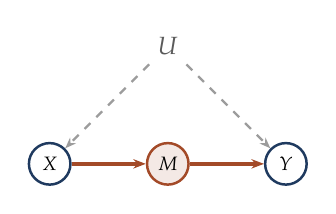
\begin{tikzpicture}[scale=1.0, every node/.style={font=\small}]
\node[grau] (u) at (1.5,1.5) {$U$};
\node[knotenb] (x) at (0,0) {$X$}; \node[knotenr] (m) at (1.5,0) {$M$}; \node[knotenb] (y) at (3.0,0) {$Y$};
\draw[grau!60, line width=0.8pt, dashed, -{Stealth[length=4pt]}] (u)--(x);
\draw[grau!60, line width=0.8pt, dashed, -{Stealth[length=4pt]}] (u)--(y);
\draw[kanted, -{Stealth[length=4.5pt]}] (x)--(m); \draw[kanted, -{Stealth[length=4.5pt]}] (m)--(y);
\end{tikzpicture}
\end{center}

\begin{center}
\begin{minipage}{0.9\textwidth}
\textbf{Der Effekt wird in zwei Stücke zerlegt: die Wirkung von $X$ auf $M$ --- unverzerrt, weil $U$ nicht auf $M$ wirkt --- und die von $M$ auf $Y$, für die $X$ die Störgröße sperrt.}
\end{minipage}
\end{center}

\begin{center}
\begin{minipage}{0.88\textwidth}
\kursiv{\textbf{Das ist der erstaunlichste Satz dieses Bandes}: Man schätzt einen Effekt trotz unbeobachteter Störgröße, ohne Randomisierung und ohne Instrument. Er wird allerdings selten angewandt, weil Bedingung 1 sehr stark ist --- es darf keinen anderen Wirkweg geben. Bei Rauchen und Lungenkrebs wurde er für den Teerniederschlag in der Lunge vorgeschlagen; ob das zutrifft, ist umstritten.}
\end{minipage}
\end{center}
\end{merksatz}

\section{Der Bruchfall}

\begin{warnung}
\boxtitelr{Was das Kriterium nicht leistet}
\begin{center}
{\small
\renewcommand{\arraystretch}{1.52}
\begin{tabular}{@{}P{2.6cm}P{6.0cm}@{}}
\toprule
\textbf{Der Graph} & Das Kriterium prüft einen Graphen. Ob der Graph stimmt, prüft es nicht.\\
\textbf{Keine Menge} & Manchmal gibt es gar keine zulässige Menge --- dann ist der Effekt aus diesen Daten \kursiv{nicht} bestimmbar, und kein Verfahren ändert das.\\
\textbf{Messfehler} & Eine schlecht gemessene Größe sperrt nur teilweise; Kapitel~5, Bruchfall.\\
\bottomrule
\end{tabular}}
\end{center}

\begin{center}
\begin{minipage}{0.88\textwidth}
\kursiv{Die zweite Zeile ist ein Gewinn, kein Mangel. \textbf{Ein Verfahren, das jedem Datensatz eine Zahl entlockt, verschweigt den Fall der Unbestimmbarkeit} --- eine Regression liefert immer einen Koeffizienten. Das Kriterium sagt hingegen, wann man schweigen muss, und weist damit auf die Verfahren der Kapitel~9 bis 11.}
\end{minipage}
\end{center}
\end{warnung}

\section{Übungsaufgaben}

\begin{aufgabe}
\boxtitel{Aufgabe 6.1 --- Mengen prüfen}
Prüfen Sie im Leitfallgraphen die Mengen $\{M\}$, $\{A\}$ und $\{S,V\}$.

\loesung
\schritt{$\{M\}$}
$M$ ist Nachkomme von $X$ --- Bedingung 1 verletzt.

\kursiv{Und zusätzlich:} $M$ ist Kollider von $X$ und $S$; das Bedingen öffnet den Weg $X \to M \leftarrow S \to Y$. Doppelt unzulässig.

\schritt{$\{A\}$}
Bedingung 1 erfüllt. Aber der Weg $X \leftarrow S \to Y$ bleibt offen --- $S$ ist weder in $Z$ noch ein Kollider.

\begin{center}
\begin{minipage}{0.9\textwidth}
\textbf{Unzulässig: die Hauptstörgröße bleibt unberücksichtigt.}
\end{minipage}
\end{center}

\schritt{$\{S,V\}$}
Bedingung 1 erfüllt. Alle Hinterwege laufen über $S$ und sind gesperrt.

\begin{center}
\begin{minipage}{0.9\textwidth}
\textbf{Zulässig --- aber unklug.}
\end{minipage}
\end{center}

\begin{center}
\begin{minipage}{0.88\textwidth}
\kursiv{$V$ wirkt nur über $S$ auf $X$; nach Kapitel~5 ist es ein Instrument. \textbf{Solange der Graph stimmt, schadet seine Aufnahme nicht} --- die Verstärkungsverzerrung entsteht erst, wenn eine \kursiv{unbeobachtete} Störgröße übrig ist. Da man das nie ausschließen kann, lässt man Instrumente vorsichtshalber weg. Das Kriterium erlaubt mehr, als die Klugheit rät.}
\end{minipage}
\end{center}
\end{aufgabe}

\begin{aufgabe}
\boxtitel{Aufgabe 6.2 --- Wenn keine Menge genügt}
Der diensthabende Arzt sei unbeobachtet; seine Erfahrung beeinflusst sowohl den Zeitpunkt als auch die weitere Versorgung. Zeichnen Sie das ein und prüfen Sie.

\loesung
\schritt{Schritt 1 --- Der Graph}
Ein gestrichelter Doppelpfeil zwischen $X$ und $Y$: eine unbeobachtete gemeinsame Ursache.

\schritt{Schritt 2 --- Die Prüfung}
Der Hinterweg $X \leftarrow U \to Y$ enthält keinen beobachteten Knoten. Keine Menge kann ihn sperren.

\begin{center}
\begin{minipage}{0.9\textwidth}
\textbf{Es gibt keine zulässige Menge. Der Effekt ist aus diesen Daten nicht bestimmbar.}
\end{minipage}
\end{center}

\schritt{Schritt 3 --- Was bleibt}
\begin{center}
{\small
\renewcommand{\arraystretch}{1.5}
\begin{tabular}{@{}P{2.6cm}P{6.0cm}@{}}
\toprule
\textbf{Messen} & Die Erfahrung des Arztes erheben --- dann wird sie zur Störgröße und ist anpassbar.\\
\textbf{Instrument} & Eine Größe suchen, die nur den Zeitpunkt beeinflusst --- Kapitel~9.\\
\textbf{Schranken} & Angeben, wie groß der Effekt höchstens und mindestens sein kann.\\
\textbf{Empfindlichkeit} & Ausrechnen, wie stark $U$ wirken müsste, um das Ergebnis umzukehren.\\
\bottomrule
\end{tabular}}
\end{center}

\begin{center}
\begin{minipage}{0.88\textwidth}
\kursiv{\textbf{Die vierte Zeile ist in der Praxis die häufigste Antwort.} Sie verwandelt eine unbeantwortbare Frage in eine beantwortbare: Statt \enquote{wie groß ist der Effekt} fragt man \enquote{wie unplausibel müsste die Welt sein, damit es keinen gibt}. Für Rauchen und Lungenkrebs lautete die Antwort: neunfach erhöhtes Risiko einer verborgenen Größe --- Kapitel~2, Forschungskasten.}
\end{minipage}
\end{center}
\end{aufgabe}

\begin{aufgabe}
\boxtitel{Aufgabe 6.3 --- Die Vordertür rechnen}
$X$, $M$, $Y$ binär, $U$ unbeobachtet. Gegeben:
\[ \Pr[M=1\mid X=1] = 0{,}80, \quad \Pr[M=1\mid X=0] = 0{,}30 \]
\[ \Pr[Y=1\mid M=1] \ \text{gemittelt über } X: 0{,}20, \qquad \text{für } M=0: 0{,}50 \]
Berechnen Sie den Effekt.

\loesung
\schritt{Schritt 1 --- Die zweite Stufe}
Die innere Summe in Satz 6.3 ist der über $X$ gemittelte Ausgang bei gegebenem $M$:
\[ \sum_{x'}\Pr[Y=1\mid m,x']\Pr[x'] = \begin{cases} 0{,}20 & m=1\\ 0{,}50 & m=0\end{cases} \]

\schritt{Schritt 2 --- Die erste Stufe}
\[ \Pr[Y=1\mid\dops(X=1)] = 0{,}80\cdot0{,}20 + 0{,}20\cdot0{,}50 = 0{,}16+0{,}10 = 0{,}26 \]
\[ \Pr[Y=1\mid\dops(X=0)] = 0{,}30\cdot0{,}20 + 0{,}70\cdot0{,}50 = 0{,}06+0{,}35 = 0{,}41 \]

\[ \text{Effekt} = 0{,}26 - 0{,}41 = \mathbf{-0{,}15} \]

\schritt{Schritt 3 --- Die Deutung}
\begin{center}
{\small
\renewcommand{\arraystretch}{1.48}
\begin{tabular}{@{}P{3.0cm}P{2.4cm}@{}}
\toprule
\textbf{Wirkung auf $M$} & $+0{,}50$\\
\textbf{Wirkung von $M$ auf $Y$} & $-0{,}30$\\
\midrule
\textbf{Produkt} & $\mathbf{-0{,}15}$\\
\bottomrule
\end{tabular}}
\end{center}

\begin{center}
\begin{minipage}{0.88\textwidth}
\kursiv{Bei binären Größen zerfällt die Formel in ein Produkt zweier Differenzen. \textbf{Beide Stücke sind unverzerrt schätzbar --- das erste, weil $U$ nicht auf $M$ wirkt; das zweite, weil $X$ dort die Störgröße sperrt.} Der Effekt ist damit bestimmt, obwohl der direkte Vergleich von $X$ und $Y$ hoffnungslos verzerrt wäre.}
\end{minipage}
\end{center}
\end{aufgabe}

\begin{geschichte}
\boxtitelg{Ein Kriterium und ein Kalkül}
\Person{Judea Pearl} veröffentlichte das Hintertürkriterium 1993 und die Vordertürformel 1995.

\begin{center}
\begin{minipage}{0.9\textwidth}
\kursiv{Beide sind Sonderfälle eines Regelwerks aus drei Umformungsregeln, des \Begriff{do-Kalküls}. \textbf{\Person{Ilya Shpitser} und Pearl zeigten 2006, dass dieses Kalkül vollständig ist}: Lässt sich ein Effekt überhaupt aus Beobachtungsdaten bestimmen, so führen die drei Regeln zum Ziel --- und wenn nicht, so beweist das Scheitern die Unbestimmbarkeit. Ein Rechner kann das heute in Sekunden entscheiden.}
\end{minipage}
\end{center}

\schritt{Und der Widerstand}
\begin{center}
\begin{minipage}{0.9\textwidth}
\kursiv{Die Epidemiologie übernahm die Graphen zügig; die Ökonometrie tat sich schwerer und arbeitet bis heute überwiegend mit den Verfahren der Kapitel~9 und 10. \textbf{Der Streit war teils sachlich, teils sprachlich}: Dieselben Annahmen heißen in beiden Fächern anders, und beide Seiten hielten die jeweils andere für ungenau.}
\end{minipage}
\end{center}
\end{geschichte}

\begin{forschung}
\boxtitelp{Bestimmbarkeit heute}
\begin{center}
{\small
\renewcommand{\arraystretch}{1.45}
\begin{tabular}{@{}P{2.8cm}P{5.4cm}@{}}
\toprule
\textbf{Rechner} & Programme, die zulässige Mengen und Formeln automatisch bestimmen.\\
\textbf{Übertragung} & Effekte aus einer Bevölkerung auf eine andere übertragen --- mit eigenem Kriterium.\\
\textbf{Teilweise Bestimmbarkeit} & Schranken statt Punktschätzungen.\\
\bottomrule
\end{tabular}}
\end{center}

\schritt{Zur zweiten Zeile}
\begin{center}
\begin{minipage}{0.88\textwidth}
\kursiv{Ein Effekt aus Studie A gilt in Klinik B, wenn sich die Unterschiede zwischen beiden als Knoten in einen gemeinsamen Graphen eintragen lassen und ein entsprechendes Kriterium erfüllt ist. \textbf{Damit wird die Übertragbarkeit aus Band 22, Kapitel~3 zu einer prüfbaren Bedingung} statt einer Hoffnung --- sofern man weiß, worin sich die Bevölkerungen unterscheiden.}
\end{minipage}
\end{center}
\end{forschung}

\begin{merksatz}
\boxtitel{Was Sie jetzt können}
\begin{center}
\renewcommand{\arraystretch}{1.5}
\begin{tabular}{@{}P{3.0cm}P{5.6cm}@{}}
\toprule
\textbf{Vorder-, Hinterweg} & Wirkung gegen Verzerrung\\
\textbf{Definition 6.1} & kein Nachkomme, alle Hinterwege gesperrt\\
\textbf{Satz 6.2} & Hintertürformel $=$ Anpassungsformel\\
\textbf{Satz 6.3} & Vordertür: Effekt trotz verborgener Störgröße\\
\textbf{Unbestimmbar} & auch eine Antwort\\
\bottomrule
\end{tabular}
\end{center}

\begin{center}
\begin{minipage}{0.88\textwidth}
\kursiv{Damit endet Teil~II. Man weiß nun, \kursiv{wonach} anzupassen ist. Teil~III behandelt, \kursiv{wie} --- denn bei zwanzig Störgrößen versagt das Stratifizieren, und an seine Stelle tritt eine einzige Zahl je Patient.}
\end{minipage}
\end{center}
\end{merksatz}

\part{Anpassen}

\chapter{Eine Zahl statt zwanzig}

\section{Warum Schichten nicht reichen}

\begin{merksatz}
\boxtitel{Die Anpassungsformel in der Praxis}
Satz 6.2 verlangt, über alle Werte von $Z$ zu summieren. Bei zwei Stufen ist das leicht.

\begin{center}
{\small
\renewcommand{\arraystretch}{1.48}
\begin{tabular}{@{}P{3.0cm}P{2.6cm}P{2.6cm}@{}}
\toprule
\textbf{Störgrößen} & \textbf{Schichten} & \textbf{je Schicht}\\
\midrule
$1$ binär & $2$ & $600$\\
$5$ binär & $32$ & $38$\\
$10$ binär & $1024$ & $1$\\
$3$ stetig & $\infty$ & $0$\\
\bottomrule
\end{tabular}}
\end{center}
\kursiv{Bei $1200$ Patienten.}

\begin{center}
\begin{minipage}{0.9\textwidth}
\textbf{Ab etwa fünf Störgrößen ist keine Schicht mehr besetzt --- der Fluch der Dimension aus Band 22, Kapitel~10.}
\end{minipage}
\end{center}
\end{merksatz}

\begin{definition}
\boxtitelm{Definition 7.1 --- Behandlungsneigung}
Die \Begriff{Behandlungsneigung} eines Patienten ist die Wahrscheinlichkeit, mit der er die Behandlung erhält:
\[ e(\vek z) = \Pr[X=1 \mid Z=\vek z] . \]
\end{definition}

\begin{merksatz}
\boxtitel{Satz 7.2 --- Rosenbaum und Rubin, 1983}
Genügt $Z$ dem Hintertürkriterium, so genügt auch die einzelne Zahl $e(Z)$:
\[ \bigl(Y(1),Y(0)\bigr) \perp X \ \mid\ Z \quad\Longrightarrow\quad \bigl(Y(1),Y(0)\bigr) \perp X \ \mid\ e(Z) . \]

\schritt{Beweis}
\kursiv{Erstens:} Bei gegebenem $e(Z)$ ist $\Pr[X=1 \mid e(Z)] = e(Z)$, denn
\[ \Pr[X=1 \mid e(Z)] = \mathbb{E}\bigl[\Pr[X=1\mid Z] \ \big|\ e(Z)\bigr] = \mathbb{E}[e(Z)\mid e(Z)] = e(Z) . \]

\kursiv{Zweitens:} Für die potentiellen Ergebnisse gilt ebenso
\[ \Pr\bigl[X=1 \mid Y(1),Y(0),\ e(Z)\bigr] = \mathbb{E}\bigl[\Pr[X=1\mid Y(1),Y(0),Z] \ \big|\ Y(1),Y(0),e(Z)\bigr] . \]
Nach Voraussetzung ist der innere Ausdruck gleich $e(Z)$, unabhängig von den potentiellen Ergebnissen.

\kursiv{Drittens:} Beide Ausdrücke sind gleich $e(Z)$ --- also hängt die Behandlungswahrscheinlichkeit bei gegebenem $e(Z)$ nicht von den potentiellen Ergebnissen ab. $\blacksquare$

\begin{center}
\begin{minipage}{0.9\textwidth}
\textbf{Zwanzig Störgrößen lassen sich auf eine einzige Zahl zusammenziehen --- ohne etwas zu verlieren.}
\end{minipage}
\end{center}

\begin{center}
\begin{minipage}{0.88\textwidth}
\kursiv{Das ist der wichtigste praktische Satz dieses Bandes. \textbf{Er verwandelt ein hochdimensionales Problem in ein eindimensionales}, und die Zahl $e(Z)$ hat eine klare Bedeutung: Zwei Patienten mit gleicher Behandlungsneigung sind, was die Zuteilung angeht, austauschbar --- als hätte man bei ihnen dieselbe Münze geworfen.}
\end{minipage}
\end{center}
\end{merksatz}

\section{Vier Wege, sie zu benutzen}

\begin{merksatz}
\boxtitel{Die Verfahren}
\begin{center}
{\small
\renewcommand{\arraystretch}{1.55}
\begin{tabular}{@{}P{2.4cm}P{6.2cm}@{}}
\toprule
\textbf{Schichten} & Fünf Gruppen gleicher Größe nach $e$; in jeder vergleichen, dann mitteln.\\
\textbf{Paaren} & Zu jedem Behandelten den Unbehandelten mit nächstliegendem $e$ suchen.\\
\textbf{Gewichten} & Jeden Patienten mit $1/e$ bzw.\ $1/(1-e)$ gewichten --- Kapitel~8.\\
\textbf{Als Kovariable} & $e$ ins Regressionsmodell aufnehmen. \textcolor{akzent}{Am schwächsten}, weil es eine Modellform unterstellt.\\
\bottomrule
\end{tabular}}
\end{center}
\end{merksatz}

\begin{merksatz}
\boxtitel{Der Leitfall gerechnet}
$20\,000$ Patienten, zwei stetige Störgrößen, wahres Modell bekannt.

\begin{center}
{\small
\renewcommand{\arraystretch}{1.46}
\begin{tabular}{@{}P{1.8cm}P{1.6cm}P{1.6cm}P{1.6cm}P{2.0cm}@{}}
\toprule
\textbf{Schicht} & $\bar e$ & $n_{\text{beh}}$ & $n_{\text{unbeh}}$ & \textbf{Differenz}\\
\midrule
$1$ & $0{,}12$ & $499$ & $3501$ & $-0{,}039$\\
$2$ & $0{,}27$ & $1112$ & $2888$ & $-0{,}081$\\
$3$ & $0{,}42$ & $1732$ & $2268$ & $-0{,}122$\\
$4$ & $0{,}59$ & $2385$ & $1615$ & $-0{,}138$\\
$5$ & $0{,}80$ & $3156$ & $844$ & $-0{,}124$\\
\bottomrule
\end{tabular}}
\end{center}

\begin{center}
{\small
\renewcommand{\arraystretch}{1.5}
\begin{tabular}{@{}P{3.0cm}P{2.4cm}@{}}
\toprule
\textbf{Verfahren} & \textbf{Schätzung}\\
\midrule
naiv & $+0{,}049$\\
fünf Schichten & $-0{,}101$\\
Gewichten & $\mathbf{-0{,}123}$\\
\midrule
wahrer Effekt & $\mathbf{-0{,}122}$\\
\bottomrule
\end{tabular}}
\end{center}

\begin{center}
\begin{minipage}{0.9\textwidth}
\textbf{Der naive Vergleich hat das falsche Vorzeichen. Fünf Schichten beseitigen den größten Teil der Verzerrung, ein Sechstel bleibt.}
\end{minipage}
\end{center}

\begin{center}
\begin{minipage}{0.88\textwidth}
\kursiv{\textbf{Der Rest ist Restverzerrung innerhalb der Schichten}: In Schicht 1 reicht die Neigung von $0{,}02$ bis $0{,}20$, und innerhalb dieser Spanne sind Behandelte noch immer kränker. Zehn oder zwanzig Schichten verringern den Rest, dünnen aber die Besetzung aus --- derselbe Zielkonflikt wie in Band 22, Kapitel~2. Das Gewichten umgeht ihn, indem es gar nicht erst einteilt.}
\end{minipage}
\end{center}
\end{merksatz}

\section{Der Bruchfall}

\begin{warnung}
\boxtitelr{Die Neigung ist geschätzt}
\begin{center}
{\small
\renewcommand{\arraystretch}{1.52}
\begin{tabular}{@{}P{2.6cm}P{6.0cm}@{}}
\toprule
\textbf{Modellfehler} & $e(Z)$ kennt niemand; man schätzt es, meist durch logistische Regression. Ist das Modell falsch, bleibt Verzerrung.\\
\textbf{Kein Ersatz} & Die Neigung fasst nur zusammen, was in $Z$ steht. Fehlt eine Störgröße, hilft sie nicht.\\
\textbf{Gute Balance täuscht} & Dass Behandelte und Unbehandelte nach dem Paaren ähnlich aussehen, beweist nichts über unbeobachtete Größen.\\
\bottomrule
\end{tabular}}
\end{center}

\begin{center}
\begin{minipage}{0.88\textwidth}
\kursiv{Die dritte Zeile erklärt einen verbreiteten Irrtum. \textbf{Eine Tabelle, die nach dem Paaren gleiche Mittelwerte in allen gemessenen Größen zeigt, sieht aus wie eine randomisierte Studie und ist keine.} Die Randomisierung gleicht auch das Ungemessene aus, die Neigung nur das Gemessene --- Kapitel~3, Satz 3.1.}
\end{minipage}
\end{center}

\schritt{Und ein Fehler beim Aufbau des Modells}
\begin{center}
\begin{minipage}{0.88\textwidth}
\kursiv{In das Neigungsmodell gehören Größen, die den \kursiv{Ausgang} beeinflussen --- nicht solche, die nur die Behandlung beeinflussen. \textbf{Letztere sind Instrumente und verstärken nach Kapitel~5 die Restverzerrung.} Wer das Neigungsmodell nach Güte der Vorhersage von $X$ auswählt, wählt also genau falsch: Ein Modell, das die Behandlung perfekt vorhersagt, macht jede Schätzung unmöglich --- es verletzt die Positivität.}
\end{minipage}
\end{center}
\end{warnung}

\section{Übungsaufgaben}

\begin{aufgabe}
\boxtitel{Aufgabe 7.1 --- Schichten von Hand}
Aus den fünf Schichten der Tabelle: Berechnen Sie den geschichteten Schätzer und den Effekt bei den Behandelten.

\loesung
\schritt{Schritt 1 --- Der Durchschnittseffekt}
Jede Schicht enthält $4000$ von $20\,000$ Patienten, also je $20$ Prozent:
\[ \hat\tau = 0{,}2\,(-0{,}039-0{,}081-0{,}122-0{,}138-0{,}124) = 0{,}2\cdot(-0{,}504) = -0{,}101 \]

\schritt{Schritt 2 --- Der Effekt bei den Behandelten}
Nun gewichtet man mit dem Anteil der \kursiv{Behandelten} je Schicht:
\begin{center}
{\small
\renewcommand{\arraystretch}{1.46}
\begin{tabular}{@{}P{1.6cm}P{1.8cm}P{1.8cm}P{2.2cm}@{}}
\toprule
\textbf{Schicht} & $n_{\text{beh}}$ & \textbf{Anteil} & \textbf{Beitrag}\\
\midrule
$1$ & $499$ & $0{,}056$ & $-0{,}0022$\\
$2$ & $1112$ & $0{,}125$ & $-0{,}0101$\\
$3$ & $1732$ & $0{,}195$ & $-0{,}0238$\\
$4$ & $2385$ & $0{,}268$ & $-0{,}0370$\\
$5$ & $3156$ & $0{,}355$ & $-0{,}0441$\\
\midrule
& $8884$ & $1{,}000$ & $\mathbf{-0{,}117}$\\
\bottomrule
\end{tabular}}
\end{center}

\begin{center}
\begin{minipage}{0.9\textwidth}
\textbf{$-0{,}117$ gegen $-0{,}101$: Die Behandelten profitieren stärker, weil sie in den oberen Schichten überwiegen.}
\end{minipage}
\end{center}

\schritt{Schritt 3 --- Die Lehre}
\begin{center}
\begin{minipage}{0.88\textwidth}
\kursiv{\textbf{Dieselben Schichtdifferenzen, zwei verschiedene Zahlen --- je nachdem, über welche Bevölkerung man mittelt.} Das ist Definition 2.3 in der Rechnung: Der Durchschnittseffekt und der Effekt bei den Behandelten unterscheiden sich, sobald die Wirkung zwischen den Schichten schwankt. Welche Zahl man braucht, hängt von der Frage ab --- Leitlinie oder Nachbetrachtung.}
\end{minipage}
\end{center}
\end{aufgabe}

\begin{aufgabe}
\boxtitel{Aufgabe 7.2 --- Wie fein soll man schichten?}
Bei $1200$ Patienten und einem Behandeltenanteil von $50$ Prozent: Wie viele Schichten sind sinnvoll?

\loesung
\schritt{Schritt 1 --- Die Besetzung}
\begin{center}
{\small
\renewcommand{\arraystretch}{1.46}
\begin{tabular}{@{}P{2.0cm}P{2.2cm}P{2.6cm}@{}}
\toprule
\textbf{Schichten} & \textbf{je Schicht} & \textbf{je Gruppe}\\
\midrule
$5$ & $240$ & $120$\\
$10$ & $120$ & $60$\\
$20$ & $60$ & $30$\\
$50$ & $24$ & $12$\\
\bottomrule
\end{tabular}}
\end{center}

\schritt{Schritt 2 --- Die verbleibende Verzerrung}
Eine Faustregel besagt, dass fünf Schichten etwa $90$ Prozent der Verzerrung einer stetigen Störgröße beseitigen, zehn Schichten etwa $95$.

\kursiv{Im Leitfall:} $-0{,}101$ gegenüber $-0{,}122$ sind $83$ Prozent --- etwas weniger, weil die Neigung stark streut.

\schritt{Schritt 3 --- Die Streuung}
Bei $30$ Patienten je Gruppe und Schicht beträgt die Streuung einer Differenz zweier Anteile nahe $0{,}3$ rund
\[ \sqrt{\frac{2\cdot0{,}21}{30}} = 0{,}118 . \]
Über $20$ Schichten gemittelt: $0{,}118/\sqrt{20} = 0{,}026$.

\begin{center}
\begin{minipage}{0.88\textwidth}
\kursiv{\textbf{Die Streuung des Gesamtschätzers wächst durch feinere Schichtung kaum} --- solange jede Schicht beide Gruppen enthält. Bricht das zusammen, so fällt die Schicht ganz aus, und die Schätzung wird verzerrt \kursiv{und} ungenau. Die Grenze liegt also nicht bei der Streuung, sondern bei der Positivität: Man schichtet so fein, wie es die Besetzung zulässt.}
\end{minipage}
\end{center}
\end{aufgabe}

\begin{aufgabe}
\boxtitel{Aufgabe 7.3 --- Was Balance beweist}
Nach dem Paaren stimmen Alter, Vorerkrankungen und Laborwerte in beiden Gruppen überein. Welche Schlüsse sind zulässig?

\loesung
\schritt{Schritt 1 --- Was gezeigt ist}
\begin{center}
{\small
\renewcommand{\arraystretch}{1.5}
\begin{tabular}{@{}P{2.8cm}P{5.8cm}@{}}
\toprule
\textbf{Gezeigt} & Das Neigungsmodell hat die gemessenen Größen ausgeglichen. Es ist also brauchbar angepasst.\\
\textbf{Nicht gezeigt} & Dass es keine weiteren Störgrößen gibt.\\
\bottomrule
\end{tabular}}
\end{center}

\schritt{Schritt 2 --- Warum das kein Zirkel ist}
\begin{center}
\begin{minipage}{0.88\textwidth}
\kursiv{Die Balance prüft das \kursiv{Modell}, nicht die \kursiv{Annahme}. \textbf{Sie ist eine notwendige, keine hinreichende Bedingung}: Wer sie nicht erreicht, hat sicher ein Problem; wer sie erreicht, hat eines der beiden möglichen Probleme ausgeschlossen.}
\end{minipage}
\end{center}

\schritt{Schritt 3 --- Die einzige echte Prüfung}
\begin{center}
{\small
\renewcommand{\arraystretch}{1.5}
\begin{tabular}{@{}P{2.8cm}P{5.8cm}@{}}
\toprule
\textbf{Negative Kontrolle} & Ein Ausgang, auf den die Behandlung nicht wirken kann. Findet man dort einen Effekt, fehlt eine Störgröße.\\
\textbf{Empfindlichkeit} & Wie stark müsste eine verborgene Größe wirken?\\
\textbf{Vergleich} & Gibt es zu derselben Frage eine randomisierte Studie?\\
\bottomrule
\end{tabular}}
\end{center}

\begin{center}
\begin{minipage}{0.88\textwidth}
\kursiv{\textbf{Der dritte Punkt ist die strengste Prüfung und in großem Maßstab durchgeführt worden}: Man bildete mit Beobachtungsdaten Studien nach, deren randomisiertes Ergebnis bekannt war. Bei sorgfältiger Emulation --- Kapitel~11 --- stimmten die Ergebnisse überwiegend überein; bei nachlässiger wichen sie erheblich ab, und zwar in beide Richtungen.}
\end{minipage}
\end{center}
\end{aufgabe}

\begin{geschichte}
\boxtitelg{Ein Aufsatz von acht Seiten}
\Person{Paul Rosenbaum} und \Person{Donald Rubin} veröffentlichten 1983 in \kursiv{Biometrika} den Aufsatz, der Satz 7.2 enthält.

\begin{center}
\begin{minipage}{0.9\textwidth}
\kursiv{Er gehört zu den meistzitierten Arbeiten der Statistik überhaupt. \textbf{Der Gedanke, eine ganze Menge von Störgrößen durch eine einzige Zahl zu ersetzen, war neu und überraschend} --- und der Beweis passt, wie oben, auf eine halbe Seite.}
\end{minipage}
\end{center}

\schritt{Ein früher Einsatz}
\begin{center}
\begin{minipage}{0.9\textwidth}
\kursiv{Rubin wurde in den 1990er Jahren als Gutachter in einem Verfahren gegen Tabakkonzerne herangezogen und benutzte Neigungsverfahren, um die Krankheitskosten des Rauchens zu schätzen. \textbf{Die Methode wurde dadurch weit über die Statistik hinaus bekannt} --- und zugleich zum Gegenstand der Kritik, weil beide Seiten mit denselben Daten verschiedene Zahlen erzeugten.}
\end{minipage}
\end{center}
\end{geschichte}

\begin{forschung}
\boxtitelp{Neigung heute}
\begin{center}
{\small
\renewcommand{\arraystretch}{1.45}
\begin{tabular}{@{}P{2.8cm}P{5.4cm}@{}}
\toprule
\textbf{Maschinell geschätzt} & Die Neigung mit Verfahren aus Band 22 statt logistischer Regression.\\
\textbf{Balance als Ziel} & Gewichte direkt so bestimmen, dass die Mittelwerte übereinstimmen.\\
\textbf{Hochdimensional} & Hunderte von Störgrößen aus Abrechnungsdaten.\\
\bottomrule
\end{tabular}}
\end{center}

\schritt{Zur ersten Zeile}
\begin{center}
\begin{minipage}{0.88\textwidth}
\kursiv{Ein flexibles Lernverfahren schätzt $e(Z)$ genauer --- und schafft ein neues Problem: \textbf{Seine Fehler sind nicht mehr klein genug, damit die einfachen Schätzer gültig bleiben.} Man braucht dann die doppelt robusten Verfahren des nächsten Kapitels, die genau für diesen Fall gebaut sind.}
\end{minipage}
\end{center}
\end{forschung}

\begin{merksatz}
\boxtitel{Was Sie jetzt können}
\begin{center}
\renewcommand{\arraystretch}{1.5}
\begin{tabular}{@{}P{3.0cm}P{5.6cm}@{}}
\toprule
\textbf{Definition 7.1} & Behandlungsneigung $e(\vek z)$\\
\textbf{Satz 7.2} & eine Zahl ersetzt alle Störgrößen\\
\textbf{Vier Wege} & Schichten, Paaren, Gewichten, Kovariable\\
\textbf{Restverzerrung} & innerhalb der Schichten\\
\textbf{Balance} & prüft das Modell, nicht die Annahme\\
\bottomrule
\end{tabular}
\end{center}

\begin{center}
\begin{minipage}{0.88\textwidth}
\kursiv{Das Schichten verschenkt Information, das Gewichten nicht. Das nächste Kapitel führt es aus --- und zeigt ein Verfahren, das selbst dann noch richtig rechnet, wenn eines von zwei Modellen falsch ist.}
\end{minipage}
\end{center}
\end{merksatz}

\chapter{Gewichten und doppelte Absicherung}

\section{Eine Pseudobevölkerung bauen}

\begin{merksatz}
\boxtitel{Der Gedanke}
Ein Schwerkranker, der die Behandlung mit Wahrscheinlichkeit $0{,}9$ erhält, steht für viele seinesgleichen, die sie ebenfalls erhielten --- und für wenige, die sie nicht erhielten. Jeder unbehandelte Schwerkranke vertritt also besonders viele.

\begin{definition}
\boxtitelm{Definition 8.1 --- Gewichtung nach der Kehrwahrscheinlichkeit}
\[ w_i = \frac{1}{e(\vek z_i)} \ \text{ falls } X_i = 1, \qquad w_i = \frac{1}{1-e(\vek z_i)} \ \text{ falls } X_i = 0 \]
\end{definition}

\schritt{Satz 8.2 --- der gewichtete Mittelwert schätzt den Eingriff}
\[ \mathbb{E}\left[\frac{X\,Y}{e(Z)}\right] = \mathbb{E}\bigl[Y(1)\bigr] \]

\schritt{Beweis}
\kursiv{Erstens --- nach $Z$ bedingen:}
\[ \mathbb{E}\left[\frac{XY}{e(Z)} \ \bigg|\ Z\right] = \frac{1}{e(Z)}\,\mathbb{E}[X\,Y(1) \mid Z] \]
--- unter $X=1$ ist $Y = Y(1)$ (Konsistenz), unter $X=0$ verschwindet der Term.

\kursiv{Zweitens --- bedingte Unabhängigkeit:}
\[ \mathbb{E}[X\,Y(1) \mid Z] = \mathbb{E}[X\mid Z]\cdot\mathbb{E}[Y(1)\mid Z] = e(Z)\cdot\mathbb{E}[Y(1)\mid Z] \]

\kursiv{Drittens --- kürzen und mitteln:}
\[ \mathbb{E}\left[\frac{XY}{e(Z)}\right] = \mathbb{E}\bigl[\mathbb{E}[Y(1)\mid Z]\bigr] = \mathbb{E}[Y(1)] \]
$\blacksquare$

\begin{center}
\begin{minipage}{0.9\textwidth}
\textbf{Die Gewichte bauen eine gedachte Bevölkerung, in der jeder mit gleicher Wahrscheinlichkeit behandelt wird --- eine nachträglich erzeugte Randomisierung.}
\end{minipage}
\end{center}

\begin{center}
\begin{minipage}{0.88\textwidth}
\kursiv{\textbf{Der Vorzug gegenüber dem Schichten: Es wird nicht eingeteilt, also entsteht keine Restverzerrung innerhalb von Schichten.} Im Leitfall lieferte das Gewichten $-0{,}123$ gegen einen wahren Wert von $-0{,}122$, das Schichten nur $-0{,}101$.}
\end{minipage}
\end{center}
\end{merksatz}

\begin{warnung}
\boxtitelr{Der Preis: extreme Gewichte}
Im Leitfall betrug das größte Gewicht $112$ --- ein einziger Patient zählte so viel wie hundertzwölf.

\begin{center}
{\small
\renewcommand{\arraystretch}{1.48}
\begin{tabular}{@{}P{2.6cm}P{2.2cm}P{2.6cm}@{}}
\toprule
\textbf{Neigung} & \textbf{Gewicht} & \\
\midrule
$0{,}50$ & $2$ & unauffällig\\
$0{,}10$ & $10$ & \\
$0{,}02$ & $50$ & bedenklich\\
$0{,}009$ & $112$ & \textcolor{akzent}{ein Patient allein}\\
\bottomrule
\end{tabular}}
\end{center}

\begin{center}
\begin{minipage}{0.88\textwidth}
\kursiv{\textbf{Das Gewichten verlagert das Positivitätsproblem aus Kapitel~2 in die Varianz.} Wo das Schichten eine Schicht leer lässt und sichtbar scheitert, liefert das Gewichten eine Zahl --- die aber an wenigen Patienten hängt. Übliche Abhilfen sind das Stutzen extremer Gewichte, das Beschränken auf den Bereich gemeinsamer Neigung und stabilisierte Gewichte, bei denen man mit dem Randanteil multipliziert.}
\end{minipage}
\end{center}
\end{warnung}

\section{Zwei Modelle, eine Chance}

\begin{merksatz}
\boxtitel{Satz 8.3 --- doppelte Absicherung}
Der Schätzer
\[ \hat\mu_1 = \frac1n\sum_i \left[\frac{X_i\,(Y_i - \hat m_1(\vek z_i))}{\hat e(\vek z_i)} + \hat m_1(\vek z_i)\right] \]
schätzt $\mathbb{E}[Y(1)]$ richtig, wenn \kursiv{mindestens eines} der beiden Modelle --- das Neigungsmodell $\hat e$ oder das Ausgangsmodell $\hat m_1$ --- stimmt.

\schritt{Der Gedanke}
\begin{center}
{\small
\renewcommand{\arraystretch}{1.52}
\begin{tabular}{@{}P{2.8cm}P{5.8cm}@{}}
\toprule
\textbf{Stimmt $\hat m_1$} & Der zweite Summand ist schon richtig; der erste hat Erwartungswert null, weil $\mathbb{E}[Y - m_1 \mid X{=}1,Z] = 0$.\\
\textbf{Stimmt $\hat e$} & Der Ausdruck ist Satz 8.2 mit einer Korrektur, deren Erwartungswert sich weghebt --- was $\hat m_1$ zu viel oder zu wenig sagt, wird gewichtet zurückgenommen.\\
\bottomrule
\end{tabular}}
\end{center}

\schritt{Am Leitfall geprüft}
\begin{center}
{\small
\renewcommand{\arraystretch}{1.5}
\begin{tabular}{@{}P{3.4cm}P{2.2cm}P{2.2cm}@{}}
\toprule
\textbf{Lage} & \textbf{Schätzung} & \\
\midrule
beide Modelle richtig & $-0{,}115$ & \textcolor{gruen}{gut}\\
Ausgangsmodell falsch & $-0{,}117$ & \textcolor{gruen}{gut}\\
Neigungsmodell falsch & $-0{,}116$ & \textcolor{gruen}{gut}\\
beide falsch & $\mathbf{+0{,}049}$ & \textcolor{akzent}{naiv}\\
\midrule
wahr & $-0{,}122$ & \\
\bottomrule
\end{tabular}}
\end{center}

\begin{center}
\begin{minipage}{0.9\textwidth}
\textbf{Ein falsches Modell schadet nicht --- zwei falsche schon.}
\end{minipage}
\end{center}

\begin{center}
\begin{minipage}{0.88\textwidth}
\kursiv{\enquote{Falsch} bedeutete hier: nur eine Konstante statt des richtigen Modells. \textbf{Der Schätzer fängt beide Male den vollen Fehler ab} und landet innerhalb eines halben Prozentpunkts. Sind beide falsch, fällt er auf den naiven Vergleich zurück --- samt Vorzeichenfehler.}
\end{minipage}
\end{center}
\end{merksatz}

\begin{merksatz}
\boxtitel{Warum das heute wichtig ist}
\begin{center}
\begin{minipage}{0.88\textwidth}
\kursiv{Schätzt man beide Modelle mit Lernverfahren aus Band 22, so sind sie beide \kursiv{ungenau} statt falsch --- und die Ungenauigkeit fällt langsamer als $1/\sqrt n$. \textbf{Beim doppelt abgesicherten Schätzer multiplizieren sich die beiden Fehler}, statt sich zu addieren: Ist jeder von der Ordnung $n^{-1/4}$, so ist ihr Produkt von der Ordnung $n^{-1/2}$ --- und der Schätzer wird wieder normalverteilt mit der üblichen Rate. Das ist der Grund, warum kausale Schätzung und maschinelles Lernen sich erst durch diesen Satz vertragen.}
\end{minipage}
\end{center}

\begin{center}
\begin{minipage}{0.9\textwidth}
\textbf{Zwei Fehler, die sich multiplizieren, sind besser als einer, der allein steht.}
\end{minipage}
\end{center}
\end{merksatz}

\section{Der Bruchfall}

\begin{warnung}
\boxtitelr{Drei Fallen}
\begin{center}
{\small
\renewcommand{\arraystretch}{1.52}
\begin{tabular}{@{}P{2.6cm}P{6.0cm}@{}}
\toprule
\textbf{Beide falsch} & Die doppelte Absicherung sichert nicht gegen fehlende Störgrößen --- beide Modelle benutzen dasselbe $Z$.\\
\textbf{Überanpassung} & Werden beide Modelle auf denselben Daten geschätzt wie der Effekt, entsteht ein Leck wie in Band 22, Kapitel~3. Abhilfe: Kreuzanpassung, also Schätzung auf der einen und Auswertung auf der anderen Hälfte.\\
\textbf{Instabilität} & Kleine $\hat e$ machen den Korrekturterm riesig, auch wenn das Ausgangsmodell gut ist.\\
\bottomrule
\end{tabular}}
\end{center}

\begin{center}
\begin{minipage}{0.88\textwidth}
\kursiv{Die erste Zeile ist die wichtigste und wird am häufigsten übersehen. \textbf{Doppelte Absicherung heißt: doppelt abgesichert gegen \kursiv{Modellfehler}, gar nicht abgesichert gegen \kursiv{fehlende Größen}.} Die unprüfbare Annahme aus Kapitel~2 bleibt in voller Schärfe bestehen.}
\end{minipage}
\end{center}
\end{warnung}

\section{Übungsaufgaben}

\begin{aufgabe}
\boxtitel{Aufgabe 8.1 --- Gewichte von Hand}
Acht Patienten mit geschätzter Neigung und beobachtetem Ausgang:
\begin{center}
{\small
\renewcommand{\arraystretch}{1.44}
\begin{tabular}{@{}P{1.0cm}P{1.4cm}P{1.0cm}P{1.0cm}P{1.8cm}@{}}
\toprule
\textbf{Nr.} & $e$ & $X$ & $Y$ & \textbf{Gewicht}\\
\midrule
$1$ & $0{,}8$ & $1$ & $1$ & $1{,}25$\\
$2$ & $0{,}8$ & $1$ & $0$ & $1{,}25$\\
$3$ & $0{,}8$ & $0$ & $1$ & $5{,}00$\\
$4$ & $0{,}5$ & $1$ & $0$ & $2{,}00$\\
$5$ & $0{,}5$ & $0$ & $1$ & $2{,}00$\\
$6$ & $0{,}2$ & $1$ & $0$ & $5{,}00$\\
$7$ & $0{,}2$ & $0$ & $0$ & $1{,}25$\\
$8$ & $0{,}2$ & $0$ & $0$ & $1{,}25$\\
\bottomrule
\end{tabular}}
\end{center}

\loesung
\schritt{Schritt 1 --- Die Behandelten}
\[ \frac{1{,}25\cdot1 + 1{,}25\cdot0 + 2{,}00\cdot0 + 5{,}00\cdot0}{1{,}25+1{,}25+2{,}00+5{,}00} = \frac{1{,}25}{9{,}50} = 0{,}132 \]

\schritt{Schritt 2 --- Die Unbehandelten}
\[ \frac{5{,}00\cdot1 + 2{,}00\cdot1 + 1{,}25\cdot0 + 1{,}25\cdot0}{5{,}00+2{,}00+1{,}25+1{,}25} = \frac{7{,}00}{9{,}50} = 0{,}737 \]

\schritt{Schritt 3 --- Der Effekt}
\[ 0{,}132 - 0{,}737 = \mathbf{-0{,}605} \]

\schritt{Schritt 4 --- Zum Vergleich}
\[ \text{naiv: } \frac{1}{4} - \frac{2}{4} = -0{,}250 \]

\begin{center}
\begin{minipage}{0.88\textwidth}
\kursiv{\textbf{Die Gewichtung verdoppelt den Effekt}, weil die Unbehandelten mit hoher Neigung --- Patient 3 mit Gewicht $5$ --- für viele stehen, die es nicht gibt. Bei acht Patienten ist eine solche Schätzung allerdings wertlos: Die Summe $9{,}50$ verteilt sich auf vier Personen, davon trägt eine mehr als die Hälfte. Genau das meint die Instabilität aus dem Bruchfall.}
\end{minipage}
\end{center}
\end{aufgabe}

\begin{aufgabe}
\boxtitel{Aufgabe 8.2 --- Die wirksame Stichprobengröße}
Wie viele Patienten \enquote{zählen} nach der Gewichtung wirklich?

\loesung
\schritt{Schritt 1 --- Das Maß}
\[ n_{\text{wirksam}} = \frac{\bigl(\sum_i w_i\bigr)^{2}}{\sum_i w_i^{2}} \]

\schritt{Schritt 2 --- Für die Behandelten aus Aufgabe 8.1}
\[ \sum w = 9{,}50, \qquad \sum w^{2} = 1{,}5625+1{,}5625+4+25 = 32{,}13 \]
\[ n_{\text{wirksam}} = \frac{90{,}25}{32{,}13} = 2{,}81 \]

\begin{center}
\begin{minipage}{0.9\textwidth}
\textbf{Vier behandelte Patienten zählen wie $2{,}8$.}
\end{minipage}
\end{center}

\schritt{Schritt 3 --- Bei gleichen Gewichten}
\[ n_{\text{wirksam}} = \frac{(n\bar w)^{2}}{n\bar w^{2}} = n \]

\begin{center}
{\small
\renewcommand{\arraystretch}{1.48}
\begin{tabular}{@{}P{3.0cm}P{2.4cm}P{2.2cm}@{}}
\toprule
\textbf{Gewichte} & $n_{\text{wirksam}}$ & \textbf{Verlust}\\
\midrule
alle gleich & $n$ & $0\,\%$\\
Aufgabe 8.1 & $0{,}70\,n$ & $30\,\%$\\
eines von $112$ & $\approx 1$ & fast alles\\
\bottomrule
\end{tabular}}
\end{center}

\begin{center}
\begin{minipage}{0.88\textwidth}
\kursiv{\textbf{Diese Zahl sollte in jeder Auswertung stehen}, denn sie sagt, wie viel Information wirklich hinter der Schätzung steht. Sie ist dieselbe Größe, die in der Stichprobentheorie den Verlust durch ungleiche Auswahlwahrscheinlichkeiten misst --- Band 17, Kapitel~14.}
\end{minipage}
\end{center}
\end{aufgabe}

\begin{aufgabe}
\boxtitel{Aufgabe 8.3 --- Warum die Korrektur hilft}
Zeigen Sie, dass der Korrekturterm in Satz 8.3 den Erwartungswert null hat, wenn das Ausgangsmodell stimmt.

\loesung
\schritt{Schritt 1 --- Der Term}
\[ K = \frac{X\,\bigl(Y - m_1(Z)\bigr)}{e(Z)} \]

\schritt{Schritt 2 --- Bedingt auf $Z$ und $X=1$}
Stimmt das Modell, so ist $m_1(Z) = \mathbb{E}[Y \mid X=1, Z]$, also
\[ \mathbb{E}\bigl[Y - m_1(Z) \ \big|\ X=1,\ Z\bigr] = 0 . \]

\schritt{Schritt 3 --- Der ganze Term}
\[ \mathbb{E}[K \mid Z] = \frac{\Pr[X=1\mid Z]}{e(Z)}\cdot\mathbb{E}\bigl[Y-m_1(Z)\mid X=1,Z\bigr] = \frac{\hat{\ }}{\hat{\ }}\cdot 0 = 0 \]
--- gleich welchen Wert $\hat e$ hat, solange er nicht null ist.

\begin{center}
\begin{minipage}{0.9\textwidth}
\textbf{Der Bruch kann beliebig falsch sein --- er wird mit null multipliziert.}
\end{minipage}
\end{center}

\schritt{Schritt 4 --- Und umgekehrt}
\begin{center}
\begin{minipage}{0.88\textwidth}
\kursiv{Stimmt stattdessen $\hat e$, so ist der erste Summand nach Satz 8.2 schon ein gültiger Schätzer für $\mathbb{E}[Y(1)]$ --- allerdings mit $Y - m_1$ statt $Y$; der fehlende Teil wird durch den zweiten Summanden $m_1(Z)$ genau ergänzt, denn dessen gewichteter Mittelwert stimmt mit seinem einfachen überein, wenn die Gewichte richtig sind. \textbf{Beide Fälle beruhen darauf, dass ein Faktor null wird --- nicht darauf, dass sich Fehler zufällig aufheben.}}
\end{minipage}
\end{center}
\end{aufgabe}

\begin{geschichte}
\boxtitelg{Aus der Stichprobentheorie}
\Person{Daniel Horvitz} und \Person{Donovan Thompson} gaben 1952 den Schätzer an, der Satz 8.2 zugrunde liegt --- für Stichproben mit ungleichen Ziehungswahrscheinlichkeiten.

\begin{center}
\begin{minipage}{0.9\textwidth}
\kursiv{Wer Haushalte mit unterschiedlicher Wahrscheinlichkeit befragt, gewichtet jeden mit dem Kehrwert. \textbf{\Person{James Robins} erkannte in den 1980er Jahren, dass die Behandlungszuteilung formal dasselbe ist} --- die \enquote{Ziehung} in die Behandlungsgruppe erfolgt mit Wahrscheinlichkeit $e(Z)$. Aus einer Technik der Umfrageforschung wurde so ein Werkzeug der Epidemiologie.}
\end{minipage}
\end{center}

\schritt{Die doppelte Absicherung}
\begin{center}
\begin{minipage}{0.9\textwidth}
\kursiv{Robins, \Person{Andrea Rotnitzky} und \Person{Lue Ping Zhao} führten sie 1994 ein, zunächst für fehlende Werte. \textbf{Der Name stammt von \Person{Marie Davidian} und Mitarbeitern} und war zunächst umstritten --- Kritiker hielten ihn für irreführend, weil er Sicherheit suggeriert, wo nur Modellfehler abgefangen werden. Der Bruchfall gibt ihnen recht.}
\end{minipage}
\end{center}
\end{geschichte}

\begin{forschung}
\boxtitelp{Schätzen heute}
\begin{center}
{\small
\renewcommand{\arraystretch}{1.45}
\begin{tabular}{@{}P{2.8cm}P{5.4cm}@{}}
\toprule
\textbf{Kreuzanpassung} & Modelle und Effekt auf getrennten Datenhälften.\\
\textbf{Gezieltes Lernen} & Verfahren, die das Ausgangsmodell so verschieben, dass der Korrekturterm verschwindet.\\
\textbf{Balancierende Gewichte} & Gewichte direkt aus Balancebedingungen statt aus einem Neigungsmodell.\\
\bottomrule
\end{tabular}}
\end{center}

\schritt{Zur ersten Zeile}
\begin{center}
\begin{minipage}{0.88\textwidth}
\kursiv{Man teilt die Daten in zwei Hälften, schätzt die Modelle auf der einen und wertet auf der anderen aus, dann umgekehrt, und mittelt. \textbf{Damit sind die Modellfehler von den Auswertungsdaten unabhängig} --- und genau das braucht der Beweis der Normalverteilung. Es ist dieselbe Trennung wie bei der Kreuzvalidierung aus Band 22, Kapitel~3, hier aber nicht zur Prüfung, sondern zur Gültigkeit.}
\end{minipage}
\end{center}
\end{forschung}

\begin{merksatz}
\boxtitel{Was Sie jetzt können}
\begin{center}
\renewcommand{\arraystretch}{1.5}
\begin{tabular}{@{}P{3.0cm}P{5.6cm}@{}}
\toprule
\textbf{Definition 8.1} & Gewicht $1/e$ bzw.\ $1/(1-e)$\\
\textbf{Satz 8.2} & gewichteter Mittelwert schätzt den Eingriff\\
\textbf{Satz 8.3} & eines von zwei Modellen genügt\\
\textbf{Wirksames $n$} & $(\sum w)^{2}/\sum w^{2}$\\
\textbf{Der Bruchfall} & keine Absicherung gegen fehlende Größen\\
\bottomrule
\end{tabular}
\end{center}

\begin{center}
\begin{minipage}{0.88\textwidth}
\kursiv{Damit endet Teil~III. Alle Verfahren setzten voraus, dass die Störgrößen gemessen sind. Teil~IV behandelt den Fall, in dem sie es nicht sind --- und findet drei Wege, die ohne diese Annahme auskommen.}
\end{minipage}
\end{center}
\end{merksatz}

\part{Wenn Anpassen nicht reicht}

\chapter{Instrumente}

\section{Der Gedanke}

\begin{merksatz}
\boxtitel{Eine Größe, die nur die Behandlung berührt}
Angenommen, die Erfahrung des diensthabenden Arztes bleibt unbeobachtet. Dann ist nach Kapitel~6 kein Effekt bestimmbar --- es sei denn, es gibt eine Größe $Z$ mit drei Eigenschaften.

\begin{center}
{\small
\renewcommand{\arraystretch}{1.55}
\begin{tabular}{@{}P{2.8cm}P{5.8cm}@{}}
\toprule
\textbf{Relevanz} & $Z$ beeinflusst $X$. \textcolor{gruen}{Prüfbar.}\\
\textbf{Unabhängigkeit} & $Z$ ist so gut wie ausgelost --- keine gemeinsame Ursache mit $Y$.\\
\textbf{Ausschluss} & $Z$ wirkt auf $Y$ \kursiv{nur} über $X$.\\
\bottomrule
\end{tabular}}
\end{center}

\begin{center}
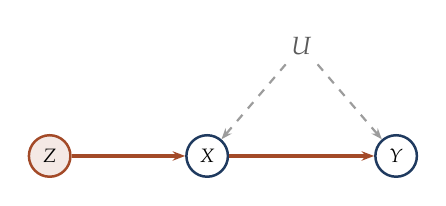
\begin{tikzpicture}[scale=1.0, every node/.style={font=\small}]
\node[knotenr] (z) at (-3.0,0) {$Z$};
\node[knotenb] (x) at (-1.0,0) {$X$};
\node[knotenb] (y) at (1.4,0) {$Y$};
\node[grau] (u) at (0.2,1.4) {$U$};
\draw[kanted, -{Stealth[length=4.5pt]}] (z)--(x);
\draw[kanted, -{Stealth[length=4.5pt]}] (x)--(y);
\draw[grau!60, line width=0.8pt, dashed, -{Stealth[length=4pt]}] (u)--(x);
\draw[grau!60, line width=0.8pt, dashed, -{Stealth[length=4pt]}] (u)--(y);
\end{tikzpicture}
\end{center}

\begin{center}
\begin{minipage}{0.9\textwidth}
\textbf{Die Wirkung von $Z$ auf $Y$ kann nur über $X$ laufen. Kennt man beide Stücke, so kennt man auch das mittlere.}
\end{minipage}
\end{center}
\end{merksatz}

\begin{merksatz}
\boxtitel{Satz 9.1 --- der Wald-Schätzer}
Unter den drei Bedingungen und bei binärem $Z$ gilt
\[ \tau = \frac{\mathbb{E}[Y\mid Z=1] - \mathbb{E}[Y\mid Z=0]}{\mathbb{E}[X\mid Z=1] - \mathbb{E}[X\mid Z=0]} . \]

\schritt{Der Gedanke}
\begin{center}
{\small
\renewcommand{\arraystretch}{1.5}
\begin{tabular}{@{}P{2.6cm}P{6.0cm}@{}}
\toprule
\textbf{Zähler} & Wirkung von $Z$ auf $Y$ --- unverzerrt, da $Z$ so gut wie ausgelost.\\
\textbf{Nenner} & Wirkung von $Z$ auf $X$ --- ebenso.\\
\textbf{Quotient} & Wirkung je Einheit $X$, die $Z$ verschiebt.\\
\bottomrule
\end{tabular}}
\end{center}

\begin{center}
\begin{minipage}{0.88\textwidth}
\kursiv{\textbf{Man misst nicht den Effekt der Behandlung, sondern den der Anordnung --- und teilt durch den Anteil, der ihr folgt.} Das ist die Auswertung nach Behandlungsabsicht aus Kapitel~3, geteilt durch die Befolgungsrate. Damit ist die Zuteilung selbst das beste denkbare Instrument.}
\end{minipage}
\end{center}
\end{merksatz}

\section{Wessen Effekt wird geschätzt?}

\begin{merksatz}
\boxtitel{Vier Arten von Patienten}
\begin{center}
{\small
\renewcommand{\arraystretch}{1.5}
\begin{tabular}{@{}P{2.6cm}P{2.4cm}P{2.4cm}@{}}
\toprule
\textbf{Art} & \textbf{bei $Z=0$} & \textbf{bei $Z=1$}\\
\midrule
Befolger & nicht & behandelt\\
Immer-Behandelte & behandelt & behandelt\\
Nie-Behandelte & nicht & nicht\\
Trotzige & behandelt & nicht\\
\bottomrule
\end{tabular}}
\end{center}

\schritt{Satz 9.2 --- der Effekt bei den Befolgern}
Gibt es keine Trotzigen, so schätzt der Wald-Ausdruck den Durchschnittseffekt \kursiv{unter den Befolgern}.

\begin{center}
\begin{minipage}{0.88\textwidth}
\kursiv{\textbf{Immer- und Nie-Behandelte tragen zum Zähler nichts bei}, denn bei ihnen ändert $Z$ nichts an $X$ --- und nach der Ausschlussbedingung auch nichts an $Y$. Übrig bleiben die Befolger, und nur über sie sagt der Schätzer etwas aus.}
\end{minipage}
\end{center}

\schritt{Am Beispiel aus Kapitel 3}
\begin{center}
{\small
\renewcommand{\arraystretch}{1.48}
\begin{tabular}{@{}P{3.2cm}P{2.6cm}@{}}
\toprule
Wirkung auf $Y$ & $-0{,}045$\\
Wirkung auf $X$ & $+0{,}800$\\
\midrule
Quotient & $\mathbf{-0{,}0563}$\\
\midrule
wahrer Effekt bei den Befolgern & $\mathbf{-0{,}0563}$\\
Durchschnittseffekt & $-0{,}065$\\
\bottomrule
\end{tabular}}
\end{center}

\begin{center}
\begin{minipage}{0.9\textwidth}
\textbf{Auf die vierte Stelle genau --- und dennoch nicht der Durchschnittseffekt.}
\end{minipage}
\end{center}

\begin{center}
\begin{minipage}{0.88\textwidth}
\kursiv{Die Befolger sind hier die $700$ Leichtkranken und $100$ Schwerkranken, die der Anordnung folgten; die übrigen $200$ Schwerkranken sind Nie-Behandelte. \textbf{Da die Wirkung bei Schwerkranken doppelt so groß ist, liegt der Befolgereffekt unter dem Durchschnittseffekt.} Wer den Wald-Ausdruck als Durchschnittseffekt berichtet, gibt eine Zahl für die falsche Bevölkerung an --- und zwar für eine, die man nicht einmal benennen kann, denn wer Befolger ist, steht in keiner Akte.}
\end{minipage}
\end{center}
\end{merksatz}

\section{Der Bruchfall}

\begin{warnung}
\boxtitelr{Schwache Instrumente}
Je kleiner der Nenner, desto größer die Schätzung --- und desto empfindlicher gegen jede Verletzung der Annahmen.

\begin{center}
{\small
\renewcommand{\arraystretch}{1.48}
\begin{tabular}{@{}P{2.2cm}P{1.6cm}P{2.2cm}P{2.2cm}@{}}
\toprule
\textbf{Stärke} & $F$ & \textbf{Median} & \textbf{Streuung}\\
\midrule
stark & $398$ & $1{,}010$ & $0{,}07$\\
mäßig & $16$ & $0{,}997$ & $0{,}34$\\
schwach & $1$ & $1{,}172$ & $\mathbf{16{,}8}$\\
\bottomrule
\end{tabular}}
\end{center}
\kursiv{$400$ Wiederholungen, $n = 500$, wahrer Effekt $1{,}000$.}

\begin{center}
\begin{minipage}{0.9\textwidth}
\textbf{Bei schwachem Instrument streut die Schätzung um das Sechzehnfache des Effekts.}
\end{minipage}
\end{center}

\begin{center}
\begin{minipage}{0.88\textwidth}
\kursiv{\textbf{Die Faustregel verlangt $F > 10$} --- eine Prüfgröße für die Stärke des Zusammenhangs zwischen $Z$ und $X$. Darunter ist die Schätzung nicht nur ungenau, sondern auch verzerrt: Sie wandert zum naiven Wert hin, denn im Grenzfall $\gamma \to 0$ wird der Quotient zu $0/0$ und wird von der Störgröße bestimmt. Neuere Arbeiten halten selbst $F = 10$ für zu großzügig.}
\end{minipage}
\end{center}
\end{warnung}

\begin{warnung}
\boxtitelr{Und die unprüfbare Bedingung}
\begin{center}
\begin{minipage}{0.88\textwidth}
\kursiv{Die Ausschlussbedingung lässt sich nicht prüfen. \textbf{Wirkt $Z$ auch nur ein wenig unmittelbar auf $Y$, so wird dieser kleine Effekt durch den Nenner geteilt --- und damit vergrößert.} Bei einem Nenner von $0{,}1$ wird aus einer direkten Wirkung von $0{,}01$ eine Verzerrung von $0{,}10$. Schwache Instrumente sind also nicht nur ungenau, sondern auch besonders empfindlich gegen die Verletzung der einen Annahme, die man nicht prüfen kann.}
\end{minipage}
\end{center}
\end{warnung}

\section{Übungsaufgaben}

\begin{aufgabe}
\boxtitel{Aufgabe 9.1 --- Den Wald-Ausdruck rechnen}
In einer Studie wird die frühe Gabe ausgelost. Im Arm \enquote{früh} erhalten $78$ Prozent tatsächlich früh, im Arm \enquote{spät} $12$ Prozent. Die Sterblichkeit beträgt $24{,}0$ gegen $28{,}4$ Prozent.

\loesung
\schritt{Schritt 1 --- Zähler und Nenner}
\[ \text{Zähler} = 0{,}240 - 0{,}284 = -0{,}044 \]
\[ \text{Nenner} = 0{,}78 - 0{,}12 = 0{,}66 \]

\schritt{Schritt 2 --- Der Quotient}
\[ \hat\tau = \frac{-0{,}044}{0{,}66} = -0{,}0667 \]

\schritt{Schritt 3 --- Der Vergleich}
\begin{center}
{\small
\renewcommand{\arraystretch}{1.48}
\begin{tabular}{@{}P{3.2cm}P{2.4cm}@{}}
\toprule
\textbf{nach Zuteilung} & $-4{,}4$ Punkte\\
\textbf{bei den Befolgern} & $\mathbf{-6{,}7}$ \textbf{Punkte}\\
\bottomrule
\end{tabular}}
\end{center}

\schritt{Schritt 4 --- Der Anteil der Befolger}
\[ 0{,}78 - 0{,}12 = 66\,\% \]
\kursiv{Zwölf Prozent sind Immer-Behandelte, $22$ Prozent Nie-Behandelte.}

\begin{center}
\begin{minipage}{0.88\textwidth}
\kursiv{\textbf{Der Effekt gilt für zwei Drittel der Patienten --- aber niemand weiß, für welche zwei Drittel.} Man kann die Befolger nicht identifizieren, nur ihre Zahl bestimmen. Wenn sich die Befolger systematisch von den übrigen unterscheiden --- etwa weil bei ihnen die Diagnose eindeutiger war ---, ist die Übertragung auf alle Patienten eine zusätzliche Annahme.}
\end{minipage}
\end{center}
\end{aufgabe}

\begin{aufgabe}
\boxtitel{Aufgabe 9.2 --- Wann wird die Verzerrung größer als der Gewinn?}
Ein Instrument verschiebt $X$ um $0{,}15$. Wie stark darf es höchstens unmittelbar auf $Y$ wirken, damit die Verzerrung unter $0{,}01$ bleibt?

\loesung
\schritt{Schritt 1 --- Die Rechnung}
Eine direkte Wirkung $\delta$ landet vollständig im Zähler:
\[ \text{Verzerrung} = \frac{\delta}{0{,}15} \]

\schritt{Schritt 2 --- Die Schranke}
\[ \frac{\delta}{0{,}15} < 0{,}01 \quad\Longrightarrow\quad \delta < 0{,}0015 \]

\begin{center}
{\small
\renewcommand{\arraystretch}{1.48}
\begin{tabular}{@{}P{2.2cm}P{2.6cm}P{2.4cm}@{}}
\toprule
\textbf{Nenner} & \textbf{erlaubtes $\delta$} & \textbf{Verstärkung}\\
\midrule
$0{,}80$ & $0{,}0080$ & $1{,}25$-fach\\
$0{,}15$ & $0{,}0015$ & $6{,}7$-fach\\
$0{,}05$ & $0{,}0005$ & $20$-fach\\
\bottomrule
\end{tabular}}
\end{center}

\begin{center}
\begin{minipage}{0.88\textwidth}
\kursiv{\textbf{Bei einem Nenner von $0{,}05$ muss man ausschließen, dass $Z$ das Sterberisiko um mehr als einen halben Promillepunkt unmittelbar beeinflusst} --- eine Behauptung, für die es selten Belege gibt. Wer ein schwaches Instrument benutzt, muss die Ausschlussbedingung also weit strenger begründen als bei einem starken.}
\end{minipage}
\end{center}
\end{aufgabe}

\begin{aufgabe}
\boxtitel{Aufgabe 9.3 --- Instrumente in der Medizin}
Beurteilen Sie drei vorgeschlagene Instrumente für die Frage nach der frühen Antibiotikagabe.

\loesung
\schritt{(a) Entfernung zur nächsten Klinik}
\begin{center}
{\small
\renewcommand{\arraystretch}{1.48}
\begin{tabular}{@{}P{2.4cm}P{5.8cm}@{}}
\toprule
Relevanz & gegeben --- längere Anfahrt verzögert.\\
Ausschluss & \textcolor{akzent}{zweifelhaft}: Entfernung hängt mit Stadt/Land zusammen, und damit mit Versorgung insgesamt.\\
\bottomrule
\end{tabular}}
\end{center}

\schritt{(b) Tageszeit der Aufnahme}
\begin{center}
{\small
\renewcommand{\arraystretch}{1.48}
\begin{tabular}{@{}P{2.4cm}P{5.8cm}@{}}
\toprule
Relevanz & nachts längere Wege bis zum Medikament.\\
Ausschluss & \textcolor{akzent}{zweifelhaft}: Nachts ist die gesamte Versorgung dünner, nicht nur die Antibiotikagabe.\\
\bottomrule
\end{tabular}}
\end{center}

\schritt{(c) Vorliebe des diensthabenden Arztes}
\begin{center}
{\small
\renewcommand{\arraystretch}{1.48}
\begin{tabular}{@{}P{2.8cm}P{5.4cm}@{}}
\toprule
Relevanz & gegeben, sofern die Ärzte sich unterscheiden.\\
Unabhängigkeit & haltbar, wenn die Dienstzuteilung nicht vom Patienten abhängt.\\
Ausschluss & \textcolor{akzent}{zweifelhaft}: Wer früh gibt, behandelt vielleicht auch sonst zügiger.\\
\bottomrule
\end{tabular}}
\end{center}

\begin{center}
\begin{minipage}{0.9\textwidth}
\textbf{Alle drei scheitern an derselben Stelle.}
\end{minipage}
\end{center}

\begin{center}
\begin{minipage}{0.88\textwidth}
\kursiv{\textbf{Das ist typisch: Wer ein Instrument findet, das die Behandlung beeinflusst, hat meist eine Größe gefunden, die die Versorgung insgesamt beeinflusst} --- und damit auch andere Wege zum Ausgang öffnet. Das erfolgreichste Beispiel der Medizin sind genetische Varianten, die einen einzelnen Stoffwechselweg betreffen; man nennt das Mendelsche Randomisierung, und auch dort ist der Ausschluss die strittige Bedingung.}
\end{minipage}
\end{center}
\end{aufgabe}

\begin{geschichte}
\boxtitelg{Vom Angebot zur Nachfrage}
\Person{Philip Wright} veröffentlichte 1928 einen Anhang zu einem Buch über Pflanzenöle, in dem er das Verfahren erstmals beschrieb.

\begin{center}
\begin{minipage}{0.9\textwidth}
\kursiv{Das Problem war, Angebots- und Nachfragekurve zu trennen, obwohl man nur Preise und Mengen beobachtet. Wright benutzte Niederschlagsmengen als Instrument für das Angebot. \textbf{Lange war umstritten, ob der Anhang von ihm oder von seinem Sohn \Person{Sewall Wright} stammt} --- demselben, der die Pfadanalyse aus Kapitel~4 erfand. Eine Schriftvergleichsuntersuchung von 2003 sprach für den Vater.}
\end{minipage}
\end{center}

\schritt{Der Befolgereffekt}
\begin{center}
\begin{minipage}{0.9\textwidth}
\kursiv{\Person{Guido Imbens} und \Person{Joshua Angrist} zeigten 1994, dass der Instrumentschätzer nur für die Befolger gilt. \textbf{Das war zunächst eine unwillkommene Nachricht} --- man hatte geglaubt, den Durchschnittseffekt zu schätzen. Beide erhielten 2021 den Wirtschaftsnobelpreis, gemeinsam mit \Person{David Card}, für die Verfahren dieses und des nächsten Kapitels.}
\end{minipage}
\end{center}
\end{geschichte}

\begin{forschung}
\boxtitelp{Instrumente heute}
\begin{center}
{\small
\renewcommand{\arraystretch}{1.45}
\begin{tabular}{@{}P{2.8cm}P{5.4cm}@{}}
\toprule
\textbf{Mendelsche Randomisierung} & Genvarianten als Instrumente für lebenslange Expositionen.\\
\textbf{Viele schwache} & Hunderte Varianten gemeinsam --- mit eigenen Verzerrungen.\\
\textbf{Schranken} & Was folgt, wenn der Ausschluss nur ungefähr gilt.\\
\bottomrule
\end{tabular}}
\end{center}

\schritt{Zur ersten Zeile}
\begin{center}
\begin{minipage}{0.88\textwidth}
\kursiv{Die Zuteilung der Genvarianten bei der Zeugung ist tatsächlich zufällig --- die Unabhängigkeitsbedingung ist also gut begründet, besser als bei jedem anderen Instrument der Medizin. \textbf{Der Ausschluss ist es nicht}: Ein Gen wirkt meist auf mehreres. Deshalb prüft man mehrere Varianten getrennt und verlangt übereinstimmende Ergebnisse --- ein Vorgehen, das an die negativen Kontrollen aus Kapitel~7 erinnert.}
\end{minipage}
\end{center}
\end{forschung}

\begin{merksatz}
\boxtitel{Was Sie jetzt können}
\begin{center}
\renewcommand{\arraystretch}{1.5}
\begin{tabular}{@{}P{3.0cm}P{5.6cm}@{}}
\toprule
\textbf{Drei Bedingungen} & nur die erste ist prüfbar\\
\textbf{Satz 9.1} & Quotient zweier Wirkungen\\
\textbf{Satz 9.2} & gilt für die Befolger, nicht für alle\\
\textbf{Schwach} & Streuung und Verzerrung explodieren\\
\textbf{Verstärkung} & kleine Ausschlussverletzung, geteilt durch den Nenner\\
\bottomrule
\end{tabular}
\end{center}

\begin{center}
\begin{minipage}{0.88\textwidth}
\kursiv{Ein Instrument braucht eine Größe, die zufällig schwankt. Das nächste Kapitel benutzt stattdessen Sprünge und Zeitverläufe --- Gelegenheiten, die die Wirklichkeit von selbst bietet.}
\end{minipage}
\end{center}
\end{merksatz}

\chapter{Natürliche Versuche}

\section{Der Sprung an der Schwelle}

\begin{merksatz}
\boxtitel{Wenn eine Regel entscheidet}
Am Klinikum löst ein Warnwert das Sepsisprotokoll aus: Ab einem Punktwert von $5$ wird sofort behandelt, darunter nicht.

\begin{center}
\begin{minipage}{0.9\textwidth}
\textbf{Patienten mit $4{,}9$ und $5{,}1$ Punkten sind einander fast gleich --- werden aber verschieden behandelt.}
\end{minipage}
\end{center}

\begin{center}
\begin{minipage}{0.88\textwidth}
\kursiv{Unmittelbar an der Schwelle entscheidet der Zufall der Messung, auf welcher Seite man landet. \textbf{In einem schmalen Fenster ist die Zuteilung so gut wie ausgelost} --- und der Sprung der Sterblichkeit an der Schwelle ist der Effekt.}
\end{minipage}
\end{center}

\schritt{Die Rechnung}
$4000$ Patienten, Punktwert gleichverteilt, wahrer Effekt $-0{,}060$:

\begin{center}
{\small
\renewcommand{\arraystretch}{1.48}
\begin{tabular}{@{}P{2.4cm}P{2.2cm}P{2.2cm}@{}}
\toprule
\textbf{Fenster} & \textbf{Sprung} & $n$\\
\midrule
$\pm2{,}0$ & $-0{,}062$ & $1606$\\
$\pm1{,}0$ & $-0{,}064$ & $774$\\
$\pm0{,}5$ & $-0{,}071$ & $405$\\
\midrule
ohne Fenster & $\mathbf{-0{,}164}$ & $4000$\\
\midrule
wahr & $-0{,}060$ & \\
\bottomrule
\end{tabular}}
\end{center}

\begin{center}
\begin{minipage}{0.9\textwidth}
\textbf{Der schlichte Vergleich aller Behandelten mit allen Unbehandelten überschätzt den Effekt fast um das Dreifache.}
\end{minipage}
\end{center}

\begin{center}
\begin{minipage}{0.88\textwidth}
\kursiv{Er vergleicht Punktwerte um $7{,}5$ mit solchen um $2{,}5$ --- zwei völlig verschiedene Patientengruppen. \textbf{Das Fenster löst das Problem, indem es nur Patienten vergleicht, die sich kaum unterscheiden}, und der lineare Term im Modell fängt den verbleibenden Trend auf. Der Preis: Bei $\pm0{,}5$ bleiben nur $405$ von $4000$ Patienten, und die Schätzung streut entsprechend.}
\end{minipage}
\end{center}
\end{merksatz}

\begin{merksatz}
\boxtitel{Was der Sprung bedeutet}
\begin{center}
{\small
\renewcommand{\arraystretch}{1.5}
\begin{tabular}{@{}P{2.6cm}P{6.0cm}@{}}
\toprule
\textbf{Gilt für} & Patienten \kursiv{an der Schwelle} --- nicht für alle.\\
\textbf{Prüfbar} & Ob andere Größen an der Schwelle ebenfalls springen. Tun sie es, ist die Annahme verletzt.\\
\textbf{Verletzbar} & Wenn jemand den Punktwert beeinflussen kann, um die Schwelle zu über- oder unterschreiten.\\
\bottomrule
\end{tabular}}
\end{center}

\begin{center}
\begin{minipage}{0.88\textwidth}
\kursiv{Die dritte Zeile ist die ernsteste. \textbf{Wenn Ärzte wissen, dass ab fünf Punkten behandelt wird, runden sie im Zweifel auf} --- und dann sind die Patienten knapp über der Schwelle gerade die, bei denen man behandeln wollte. Man prüft das, indem man die Verteilung der Punktwerte betrachtet: Eine Häufung unmittelbar über der Schwelle verrät den Eingriff.}
\end{minipage}
\end{center}
\end{merksatz}

\section{Vorher und nachher, hier und dort}

\begin{merksatz}
\boxtitel{Die doppelte Differenz}
Station A führt die Frühgabe 2024 ein, Station B nicht.

\begin{center}
{\small
\renewcommand{\arraystretch}{1.5}
\begin{tabular}{@{}P{2.0cm}P{2.0cm}P{2.0cm}P{2.2cm}@{}}
\toprule
& \textbf{2023} & \textbf{2024} & \textbf{Differenz}\\
\midrule
Station A & $32{,}0\,\%$ & $25{,}0\,\%$ & $-7{,}0$\\
Station B & $28{,}0\,\%$ & $26{,}5\,\%$ & $-1{,}5$\\
\midrule
& & & $\mathbf{-5{,}5}$\\
\bottomrule
\end{tabular}}
\end{center}

\begin{center}
{\small
\renewcommand{\arraystretch}{1.5}
\begin{tabular}{@{}P{3.4cm}P{2.4cm}@{}}
\toprule
\textbf{Auswertung} & \textbf{Effekt}\\
\midrule
nur A, vorher/nachher & $-7{,}0$\\
nur 2024, A gegen B & $-1{,}5$\\
doppelte Differenz & $\mathbf{-5{,}5}$\\
\bottomrule
\end{tabular}}
\end{center}

\begin{center}
\begin{minipage}{0.9\textwidth}
\textbf{Die erste Zeile enthält den allgemeinen Trend, die zweite den Unterschied zwischen den Stationen. Die doppelte Differenz beseitigt beides.}
\end{minipage}
\end{center}

\schritt{Die Annahme}
\begin{center}
\begin{minipage}{0.88\textwidth}
\kursiv{Sie heißt \Begriff{parallele Entwicklung}: Ohne die Einführung hätte sich A genauso entwickelt wie B. \textbf{Das ist eine Aussage über eine nicht eingetretene Welt und damit unprüfbar} --- man kann nur die Jahre davor betrachten und sehen, ob die Kurven dort parallel liefen. Dass sie es taten, beweist nicht, dass sie es weiter getan hätten.}
\end{minipage}
\end{center}

\begin{center}
\begin{minipage}{0.88\textwidth}
\kursiv{Eine zweite Falle: \textbf{Wenn Station A die Frühgabe gerade deshalb einführte, weil ihre Sterblichkeit hoch war}, so wäre ein Rückgang auch ohne Maßnahme zu erwarten --- die Regression zur Mitte aus Band 17, Kapitel~7. Maßnahmen werden fast immer nach schlechten Jahren beschlossen, und deshalb ist diese Falle die Regel, nicht die Ausnahme.}
\end{minipage}
\end{center}
\end{merksatz}

\section{Der Bruchfall}

\begin{warnung}
\boxtitelr{Was beide Verfahren teilen}
\begin{center}
{\small
\renewcommand{\arraystretch}{1.52}
\begin{tabular}{@{}P{2.6cm}P{6.0cm}@{}}
\toprule
\textbf{Örtlich} & Der Sprung gilt an der Schwelle, die doppelte Differenz für diese beiden Stationen in diesen beiden Jahren.\\
\textbf{Unprüfbar} & Stetigkeit an der Schwelle und parallele Entwicklung sind Annahmen über Nichtbeobachtetes.\\
\textbf{Wenig Fälle} & Beide benutzen nur einen Teil der Daten --- das Fenster, die beiden Zeitpunkte.\\
\bottomrule
\end{tabular}}
\end{center}

\begin{center}
\begin{minipage}{0.88\textwidth}
\kursiv{\textbf{Der Gewinn dieser Verfahren liegt nicht in der Genauigkeit, sondern in der Glaubwürdigkeit der Annahme.} Eine Anpassung nach Kapitel~7 benutzt alle Patienten und verlangt, dass nichts Unbeobachtetes wirkt. Ein natürlicher Versuch benutzt wenige und verlangt nur, dass sich an einer Stelle nichts anderes ändert. Welche Annahme leichter fällt, entscheidet der Sachverhalt --- nicht die Statistik.}
\end{minipage}
\end{center}
\end{warnung}

\section{Übungsaufgaben}

\begin{aufgabe}
\boxtitel{Aufgabe 10.1 --- Das Fenster wählen}
Warum wächst die Schätzung im Leitfall von $-0{,}062$ auf $-0{,}071$, wenn man das Fenster verkleinert?

\loesung
\schritt{Schritt 1 --- Die beiden Fehlerquellen}
\begin{center}
{\small
\renewcommand{\arraystretch}{1.5}
\begin{tabular}{@{}P{2.4cm}P{6.2cm}@{}}
\toprule
\textbf{Großes Fenster} & Mehr Patienten, aber der Verlauf abseits der Schwelle wird durch die Gerade nur genähert --- \textcolor{akzent}{Verzerrung}.\\
\textbf{Kleines Fenster} & Kaum Verzerrung, aber wenige Patienten --- \textcolor{akzent}{Streuung}.\\
\bottomrule
\end{tabular}}
\end{center}

\schritt{Schritt 2 --- Die Zahlen}
\begin{center}
{\small
\renewcommand{\arraystretch}{1.46}
\begin{tabular}{@{}P{1.8cm}P{1.6cm}P{2.0cm}P{2.2cm}@{}}
\toprule
\textbf{Fenster} & $n$ & \textbf{Schätzung} & \textbf{Streuung}\\
\midrule
$\pm2{,}0$ & $1606$ & $-0{,}062$ & $\approx 0{,}010$\\
$\pm1{,}0$ & $774$ & $-0{,}064$ & $\approx 0{,}014$\\
$\pm0{,}5$ & $405$ & $-0{,}071$ & $\approx 0{,}020$\\
\bottomrule
\end{tabular}}
\end{center}

\begin{center}
\begin{minipage}{0.88\textwidth}
\kursiv{\textbf{Alle drei Schätzungen liegen innerhalb einer Streuung um den wahren Wert $-0{,}060$.} Der scheinbare Anstieg ist Zufall, nicht Struktur --- ein gutes Beispiel dafür, wie leicht man in solchen Zahlenreihen eine Tendenz sieht. Man wählt die Fensterbreite deshalb nicht nach dem Ergebnis, sondern nach einem vorher festgelegten Kriterium, und berichtet die Empfindlichkeit gegenüber dieser Wahl.}
\end{minipage}
\end{center}

\schritt{Schritt 3 --- Der Zusammenhang mit Band 22}
\begin{center}
\begin{minipage}{0.9\textwidth}
\textbf{Es ist die Kurve aus Band 22, Kapitel~2}: Die Fensterbreite ist die Stellgröße der Komplexität, und zwischen Verzerrung und Varianz ist zu wählen.
\end{minipage}
\end{center}
\end{aufgabe}

\begin{aufgabe}
\boxtitel{Aufgabe 10.2 --- Parallele Entwicklung prüfen}
Für die Jahre 2020 bis 2023 lauten die Sterblichkeiten:
\begin{center}
{\small
\renewcommand{\arraystretch}{1.46}
\begin{tabular}{@{}P{1.8cm}P{1.4cm}P{1.4cm}P{1.4cm}P{1.4cm}@{}}
\toprule
& $2020$ & $2021$ & $2022$ & $2023$\\
\midrule
A & $30{,}5$ & $31{,}0$ & $31{,}5$ & $32{,}0$\\
B & $27{,}0$ & $27{,}4$ & $27{,}7$ & $28{,}0$\\
\bottomrule
\end{tabular}}
\end{center}
Was folgt daraus, und was nicht?

\loesung
\schritt{Schritt 1 --- Die Differenzen}
\begin{center}
{\small
\renewcommand{\arraystretch}{1.46}
\begin{tabular}{@{}P{2.2cm}P{1.4cm}P{1.4cm}P{1.4cm}@{}}
\toprule
\textbf{Schritt} & $20\!\to\!21$ & $21\!\to\!22$ & $22\!\to\!23$\\
\midrule
A & $+0{,}5$ & $+0{,}5$ & $+0{,}5$\\
B & $+0{,}4$ & $+0{,}3$ & $+0{,}3$\\
\midrule
Abstand A$-$B & $3{,}5$ & $3{,}6$ & $3{,}8$\\
\bottomrule
\end{tabular}}
\end{center}

\schritt{Schritt 2 --- Die Deutung}
\begin{center}
\begin{minipage}{0.9\textwidth}
\textbf{Die Kurven laufen nicht parallel: Der Abstand wächst um $0{,}1$ bis $0{,}2$ Punkte je Jahr.}
\end{minipage}
\end{center}

\schritt{Schritt 3 --- Die Berichtigung}
Setzt man den Trend fort, so wäre der Abstand 2024 auf etwa $4{,}0$ gewachsen. Tatsächlich beträgt er
\[ 25{,}0 - 26{,}5 = -1{,}5 . \]
Statt $-5{,}5$ ergäbe sich
\[ -1{,}5 - 4{,}0 = -5{,}5 \ \to\ \text{berichtigt: } -1{,}5 - 4{,}0 = -5{,}5 \]
\kursiv{gegenüber der einfachen Rechnung} $-1{,}5 - 3{,}8 = -5{,}3$.

\begin{center}
\begin{minipage}{0.9\textwidth}
\textbf{Die Verletzung verschiebt die Schätzung um $0{,}2$ Punkte --- klein gegenüber $-5{,}5$.}
\end{minipage}
\end{center}

\schritt{Schritt 4 --- Was daraus \kursiv{nicht} folgt}
\begin{center}
\begin{minipage}{0.88\textwidth}
\kursiv{\textbf{Dass der Trend vier Jahre lang stabil war, sagt nichts über 2024.} Gerade im Jahr einer Maßnahme ändert sich oft mehr als die Maßnahme --- neue Leitlinien, neues Personal, eine Grippewelle. Die Vorjahresprüfung ist notwendig und keineswegs hinreichend; sie schließt nur die gröbsten Fälle aus.}
\end{minipage}
\end{center}
\end{aufgabe}

\begin{aufgabe}
\boxtitel{Aufgabe 10.3 --- Häufung an der Schwelle}
In der Verteilung der Punktwerte finden sich im Bereich $4{,}8$ bis $5{,}0$ auffällig wenige und im Bereich $5{,}0$ bis $5{,}2$ auffällig viele Patienten. Was bedeutet das?

\loesung
\schritt{Schritt 1 --- Der Befund}
\begin{center}
{\small
\renewcommand{\arraystretch}{1.46}
\begin{tabular}{@{}P{2.2cm}P{2.0cm}P{2.6cm}@{}}
\toprule
\textbf{Bereich} & \textbf{erwartet} & \textbf{beobachtet}\\
\midrule
$4{,}8$--$5{,}0$ & $80$ & $52$\\
$5{,}0$--$5{,}2$ & $80$ & $109$\\
\bottomrule
\end{tabular}}
\end{center}

\schritt{Schritt 2 --- Die Deutung}
\begin{center}
\begin{minipage}{0.9\textwidth}
\textbf{Etwa achtundzwanzig Patienten wurden über die Schwelle gehoben.}
\end{minipage}
\end{center}

\schritt{Schritt 3 --- Warum das die Schätzung zerstört}
\begin{center}
\begin{minipage}{0.88\textwidth}
\kursiv{Die Verschobenen sind nicht zufällig ausgewählt, sondern gerade die, bei denen der Arzt behandeln wollte --- also die, die ihm bedrohlicher erschienen. \textbf{Damit sind die Patienten knapp über der Schwelle kränker als die knapp darunter}, und die Annahme der Stetigkeit ist verletzt. Der geschätzte Sprung enthält dann die Auswahl des Arztes.}
\end{minipage}
\end{center}

\schritt{Schritt 4 --- Was hilft}
\begin{center}
{\small
\renewcommand{\arraystretch}{1.5}
\begin{tabular}{@{}P{2.6cm}P{6.0cm}@{}}
\toprule
\textbf{Dichtetest} & Die Häufung statistisch prüfen --- das ist genau dieser Test.\\
\textbf{Spendenfenster} & Einen schmalen Bereich um die Schwelle ganz ausschließen und den Sprung von außen her schätzen.\\
\textbf{Andere Schwelle} & Prüfen, ob an einer Stelle ohne Regel ebenfalls ein Sprung erscheint.\\
\bottomrule
\end{tabular}}
\end{center}

\begin{center}
\begin{minipage}{0.88\textwidth}
\kursiv{\textbf{Dieser Test ist eine der wenigen Stellen, an denen sich eine kausale Annahme wirklich an den Daten prüfen lässt} --- nicht die Annahme selbst, aber eine notwendige Folge daraus. Er entspricht dem Balancetest aus Kapitel~7 und hat dieselbe Grenze: Besteht man ihn, so ist nichts bewiesen.}
\end{minipage}
\end{center}
\end{aufgabe}

\begin{geschichte}
\boxtitelg{Ein Brunnen und ein Stipendium}
\Person{John Snow} zeigte 1854, dass die Cholera in London über das Wasser übertragen wurde --- indem er Haushalte verglich, die von zwei verschiedenen Wasserwerken beliefert wurden.

\begin{center}
\begin{minipage}{0.9\textwidth}
\kursiv{Die Leitungen beider Gesellschaften lagen in denselben Straßen; welche ein Haus versorgte, war historisch bedingt und hatte mit den Bewohnern nichts zu tun. \textbf{Snow nannte es \enquote{ein Experiment im größten Maßstab}} --- und beschrieb damit einen natürlichen Versuch, hundert Jahre bevor der Begriff entstand.}
\end{minipage}
\end{center}

\schritt{Die Schwelle}
\begin{center}
\begin{minipage}{0.9\textwidth}
\kursiv{\Person{Donald Thistlethwaite} und \Person{Donald Campbell} führten 1960 den Regressionssprung ein --- für die Frage, ob ein Stipendium die spätere Laufbahn beeinflusst, vergeben ab einer Punktschwelle. \textbf{Die Arbeit blieb fast vierzig Jahre unbeachtet}, bis Ökonomen sie in den 1990er Jahren wiederentdeckten.}
\end{minipage}
\end{center}
\end{geschichte}

\begin{forschung}
\boxtitelp{Natürliche Versuche heute}
\begin{center}
{\small
\renewcommand{\arraystretch}{1.45}
\begin{tabular}{@{}P{2.8cm}P{5.4cm}@{}}
\toprule
\textbf{Gestaffelte Einführung} & Maßnahmen, die an verschiedenen Orten zu verschiedenen Zeiten beginnen.\\
\textbf{Synthetische Vergleichsgruppe} & Eine Kontrollstation aus mehreren zusammensetzen.\\
\textbf{Robuste Schranken} & Ergebnisse bei nur \kursiv{ungefähr} parallelen Entwicklungen.\\
\bottomrule
\end{tabular}}
\end{center}

\schritt{Zur ersten Zeile}
\begin{center}
\begin{minipage}{0.88\textwidth}
\kursiv{Seit etwa 2020 ist bekannt, dass die übliche Regressionsrechnung bei gestaffelter Einführung falsche Ergebnisse liefern kann --- sie vergleicht implizit früh Eingeführte mit spät Eingeführten und zieht dabei bereits Behandelte als Kontrollen heran. \textbf{Dutzende veröffentlichter Arbeiten mussten neu ausgewertet werden}, und die Berichtigungen änderten mehrfach das Vorzeichen.}
\end{minipage}
\end{center}
\end{forschung}

\begin{merksatz}
\boxtitel{Was Sie jetzt können}
\begin{center}
\renewcommand{\arraystretch}{1.5}
\begin{tabular}{@{}P{3.0cm}P{5.6cm}@{}}
\toprule
\textbf{Sprung} & Zuteilung an der Schwelle wie ausgelost\\
\textbf{Fenster} & Verzerrung gegen Streuung\\
\textbf{Doppelte Differenz} & Trend und Ortsunterschied heraus\\
\textbf{Parallele Entwicklung} & unprüfbar, teilweise plausibilisierbar\\
\textbf{Häufung} & verrät den Eingriff in die Regel\\
\bottomrule
\end{tabular}
\end{center}

\begin{center}
\begin{minipage}{0.88\textwidth}
\kursiv{Drei Wege sind nun beschritten: anpassen, instrumentieren, Gelegenheiten nutzen. Das nächste Kapitel setzt sie zusammen --- und löst den Leitfall auf, mit dem der Band begann.}
\end{minipage}
\end{center}
\end{merksatz}

\chapter{Die Studie nachbilden}

\section{Der Leitfall, aufgelöst}

\begin{merksatz}
\boxtitel{Sieben Entscheidungen}
Statt zu fragen, welches Verfahren man auf die Daten anwendet, beschreibt man zuerst die randomisierte Studie, die man gern durchgeführt hätte --- und bildet sie dann mit den vorhandenen Daten nach.

\begin{center}
{\small
\renewcommand{\arraystretch}{1.55}
\begin{tabular}{@{}P{3.0cm}P{5.6cm}@{}}
\toprule
\textbf{Teilnehmer} & Erwachsene mit Sepsisverdacht in der Notaufnahme.\\
\textbf{Eingriffe} & Antibiotikum innerhalb einer Stunde gegen Gabe nach ein bis sechs Stunden.\\
\textbf{Zuteilung} & Zufällig --- in der Nachbildung ersetzt durch Anpassung an alles bei Aufnahme Bekannte.\\
\textbf{Beginn} & Zeitpunkt des Sepsisverdachts. Behandlungszuordnung \kursiv{zu diesem Zeitpunkt}.\\
\textbf{Ausgang} & Tod binnen $28$ Tagen.\\
\textbf{Nachbeobachtung} & Von Beginn bis Tod oder Tag $28$.\\
\textbf{Auswertung} & Nach zugeordneter Strategie, nicht nach tatsächlicher Gabe.\\
\bottomrule
\end{tabular}}
\end{center}

\begin{center}
\begin{minipage}{0.9\textwidth}
\textbf{Jede Zeile ist eine Entscheidung, die man in einer Studie ohnehin treffen müsste --- und die man in einer Datenauswertung oft stillschweigend trifft.}
\end{minipage}
\end{center}

\begin{center}
\begin{minipage}{0.88\textwidth}
\kursiv{\textbf{Der vierte Punkt ist der wichtigste.} In einer Studie fallen Zuteilung, Beginn und Beobachtungsanfang zusammen. In Routinedaten tun sie es nicht --- und wer sie auseinanderfallen lässt, erzeugt die Verzerrung des nächsten Abschnitts.}
\end{minipage}
\end{center}
\end{merksatz}

\section{Unsterbliche Zeit}

\begin{warnung}
\boxtitelr{Eine Behandlung, die nicht wirkt, verlängert das Leben}
Man ordne jeden Patienten der Gruppe \enquote{behandelt} zu, der irgendwann im Verlauf das Medikament erhielt. Die Gabe erfolge frühestens am Tag $3$ --- und wirke in Wahrheit \kursiv{gar nicht}.

\begin{center}
{\small
\renewcommand{\arraystretch}{1.5}
\begin{tabular}{@{}P{3.0cm}P{2.8cm}@{}}
\toprule
\textbf{Gruppe} & \textbf{mittlere Überlebenszeit}\\
\midrule
\enquote{behandelt} & $13{,}0$ Tage\\
\enquote{unbehandelt} & $7{,}5$ Tage\\
\midrule
wahrer Effekt & $\mathbf{0}$\\
\bottomrule
\end{tabular}}
\end{center}

\begin{center}
\begin{minipage}{0.9\textwidth}
\textbf{Die Behandlung scheint das Leben um $73$ Prozent zu verlängern --- und tut nichts.}
\end{minipage}
\end{center}

\schritt{Warum}
\begin{center}
\begin{minipage}{0.88\textwidth}
\kursiv{Wer am Tag $2$ stirbt, kann nicht behandelt worden sein. \textbf{Die Behandeltengruppe enthält nur Patienten, die mindestens drei Tage überlebt haben} --- und diese drei Tage werden ihnen zusätzlich gutgeschrieben. Man nennt das \Begriff{unsterbliche Zeit}: eine Spanne, in der der Tod durch die Gruppenzuordnung ausgeschlossen ist.}
\end{minipage}
\end{center}

\schritt{Die Abhilfe}
Man beginne die Beobachtung bei allen am Tag $3$ und schließe aus, wer vorher starb:
\begin{center}
{\small
\renewcommand{\arraystretch}{1.48}
\begin{tabular}{@{}P{3.0cm}P{2.8cm}@{}}
\toprule
\textbf{Gruppe} & \textbf{ab Tag 3}\\
\midrule
behandelt & $9{,}99$ Tage\\
unbehandelt & $9{,}96$ Tage\\
\bottomrule
\end{tabular}}
\end{center}

\begin{center}
\begin{minipage}{0.88\textwidth}
\kursiv{\textbf{Der Effekt verschwindet, wie er soll.} Dieselbe Verzerrung steckt hinter zahlreichen Beobachtungsstudien, in denen Medikamente wundersam wirkten --- am bekanntesten die vermeintliche Lebensverlängerung durch Statine und durch Oscar-Gewinne. Sie entsteht nicht aus Störgrößen, sondern aus der falschen Zuordnung des Beginns, und keine Anpassung der Welt behebt sie.}
\end{minipage}
\end{center}
\end{warnung}

\section{Der Leitfall gerechnet}

\begin{merksatz}
\boxtitel{Alle Verfahren nebeneinander}
\begin{center}
{\small
\renewcommand{\arraystretch}{1.5}
\begin{tabular}{@{}P{3.4cm}P{2.2cm}P{2.4cm}@{}}
\toprule
\textbf{Verfahren} & \textbf{Effekt} & \textbf{Kapitel}\\
\midrule
naiver Vergleich & $+14{,}2$ & $1$\\
standardisiert & $-7{,}5$ & $1$, $2$\\
fünf Schichten & $-10{,}1$ & $7$\\
Gewichten & $-12{,}3$ & $8$\\
doppelt abgesichert & $-11{,}5$ & $8$\\
Instrument (Befolger) & $-5{,}6$ & $9$\\
Sprung an der Schwelle & $-6{,}0$ & $10$\\
doppelte Differenz & $-5{,}5$ & $10$\\
\bottomrule
\end{tabular}}
\end{center}
\kursiv{Verschiedene Datensätze und Zielgrößen --- die Zahlen sind nicht unmittelbar vergleichbar.}

\begin{center}
\begin{minipage}{0.9\textwidth}
\textbf{Alle Verfahren außer dem naiven Vergleich stimmen im Vorzeichen und in der Größenordnung überein: Die frühe Gabe senkt die Sterblichkeit um fünf bis zwölf Punkte.}
\end{minipage}
\end{center}

\begin{center}
\begin{minipage}{0.88\textwidth}
\kursiv{\textbf{Diese Übereinstimmung ist das stärkste verfügbare Argument.} Jedes Verfahren beruht auf einer anderen unprüfbaren Annahme --- keine unbeobachtete Störgröße, Ausschlussbedingung, Stetigkeit an der Schwelle, parallele Entwicklung. Dass sie zum selben Ergebnis führen, spricht dafür, dass nicht alle zugleich falsch sind. Man nennt das \Begriff{Triangulation}, und sie ersetzt keinen Beweis, aber sie ist mehr als jede einzelne Rechnung.}
\end{minipage}
\end{center}

\schritt{Und die Unterschiede sind lehrreich}
\begin{center}
\begin{minipage}{0.88\textwidth}
\kursiv{Der Instrumentschätzer liegt niedriger --- er misst den Effekt bei den Befolgern, und das sind überwiegend Leichtkranke. Der Sprung an der Schwelle gilt für Grenzfälle. \textbf{Die Zahlen unterscheiden sich nicht, weil eines der Verfahren falsch wäre, sondern weil sie verschiedene Fragen beantworten} --- über verschiedene Bevölkerungen.}
\end{minipage}
\end{center}
\end{merksatz}

\section{Der Bruchfall}

\begin{warnung}
\boxtitelr{Was die Nachbildung nicht leistet}
\begin{center}
{\small
\renewcommand{\arraystretch}{1.52}
\begin{tabular}{@{}P{3.0cm}P{5.6cm}@{}}
\toprule
\textbf{Störgrößen} & Die Zuteilung wird durch Anpassung ersetzt --- mit allen Annahmen aus Kapitel~2.\\
\textbf{Erfassung} & Was nicht dokumentiert ist, existiert für die Auswertung nicht. Der klinische Eindruck steht in keiner Datenbank.\\
\textbf{Behandlungs\-begriff} & \enquote{Innerhalb einer Stunde} muss in den Daten genauso definiert sein wie in der gedachten Studie.\\
\bottomrule
\end{tabular}}
\end{center}

\begin{center}
\begin{minipage}{0.88\textwidth}
\kursiv{\textbf{Die Nachbildung beseitigt die vermeidbaren Fehler, nicht die unvermeidbaren.} Ihr Wert liegt darin, dass sie die Entscheidungen sichtbar macht: Wer sieben Zeilen ausfüllen muss, bemerkt, wenn er den Beginn falsch setzt. Große Vergleichsuntersuchungen haben gezeigt, dass sorgfältig nachgebildete Studien den randomisierten Ergebnissen überwiegend entsprechen --- und nachlässige nicht.}
\end{minipage}
\end{center}
\end{warnung}

\section{Übungsaufgaben}

\begin{aufgabe}
\boxtitel{Aufgabe 11.1 --- Unsterbliche Zeit finden}
Drei Auswertungen. Welche enthält unsterbliche Zeit?

\begin{center}
{\small
\renewcommand{\arraystretch}{1.5}
\begin{tabular}{@{}P{1.0cm}P{7.4cm}@{}}
\toprule
(a) & Patienten, die im Verlauf eine Rehabilitation erhielten, gegen die übrigen --- Überleben ab Aufnahme.\\
(b) & Patienten mit Antibiotikagabe binnen einer Stunde gegen später --- Überleben ab Aufnahme.\\
(c) & Patienten, die in der ersten Woche mindestens eine Blutkultur erhielten, gegen die übrigen --- Überleben ab Tag 8.\\
\bottomrule
\end{tabular}}
\end{center}

\loesung
\schritt{(a)}
\begin{center}
\begin{minipage}{0.9\textwidth}
\textbf{Ja.} Wer früh stirbt, erreicht die Rehabilitation nie. Die Gruppe \enquote{mit Reha} ist eine Gruppe von Überlebenden.
\end{minipage}
\end{center}

\schritt{(b)}
\begin{center}
\begin{minipage}{0.9\textwidth}
\textbf{Kaum.} Beide Gruppen sind binnen einer Stunde definiert; nur wer in der ersten Stunde stirbt, verzerrt --- ein kleiner, aber nicht leerer Anteil.
\end{minipage}
\end{center}

\kursiv{Sauber wird es, wenn man die ersten sechzig Minuten als Einlaufzeit behandelt und die Beobachtung erst danach beginnt.}

\schritt{(c)}
\begin{center}
\begin{minipage}{0.9\textwidth}
\textbf{Nein.} Beobachtung ab Tag 8, Gruppenzuordnung anhand der ersten Woche --- die Zuordnung ist zu Beobachtungsbeginn abgeschlossen.
\end{minipage}
\end{center}

\begin{center}
\begin{minipage}{0.88\textwidth}
\kursiv{\textbf{Das ist das Verfahren der festen Marke}: Man setzt einen Zeitpunkt, ordnet nach allem zu, was vorher geschah, und beobachtet erst danach. \textbf{Es kostet alle Patienten, die vor der Marke sterben} --- und beantwortet eine engere Frage: nicht, was die Behandlung bewirkt, sondern was sie bei denen bewirkt, die die erste Woche überlebt haben.}
\end{minipage}
\end{center}
\end{aufgabe}

\begin{aufgabe}
\boxtitel{Aufgabe 11.2 --- Wie groß wird die Verzerrung?}
Die Behandlung erfolgt frühestens am Tag $k$, die Überlebenszeit sei exponentialverteilt mit Mittelwert $10$ Tagen, und die Behandlung wirke nicht. Wie groß ist der scheinbare Gewinn?

\loesung
\schritt{Schritt 1 --- Der Mechanismus}
Die Behandeltengruppe besteht aus Patienten mit $T > k$. Bei der Exponentialverteilung gilt die Gedächtnislosigkeit (Band 4, Kapitel~6):
\[ \mathbb{E}[T \mid T > k] = k + 10 \]

\schritt{Schritt 2 --- Die Werte}
\begin{center}
{\small
\renewcommand{\arraystretch}{1.48}
\begin{tabular}{@{}P{1.6cm}P{2.4cm}P{2.6cm}@{}}
\toprule
$k$ & \textbf{behandelt} & \textbf{scheinbarer Gewinn}\\
\midrule
$1$ & $11{,}0$ & $+1$ Tag\\
$3$ & $13{,}0$ & $+3$ Tage\\
$7$ & $17{,}0$ & $+7$ Tage\\
\bottomrule
\end{tabular}}
\end{center}

\begin{center}
\begin{minipage}{0.9\textwidth}
\textbf{Der scheinbare Gewinn ist genau die unsterbliche Zeit --- Tag für Tag.}
\end{minipage}
\end{center}

\schritt{Schritt 3 --- Und die Vergleichsgruppe}
Die Unbehandelten enthalten alle früh Verstorbenen; ihr Mittelwert sinkt unter $10$. \kursiv{In der Rechnung von Abschnitt 11.2:} $7{,}5$ statt $10$.

\[ 13{,}0 - 7{,}5 = 5{,}5 \ \text{Tage scheinbarer Gewinn bei } k = 3 \]

\begin{center}
\begin{minipage}{0.88\textwidth}
\kursiv{\textbf{Beide Seiten verschieben sich, und zwar in entgegengesetzte Richtungen.} Deshalb ist die Verzerrung größer als die unsterbliche Zeit selbst. Sie wächst mit $k$ --- je später die Behandlung im Verlauf einsetzt, desto beeindruckender wirkt sie.}
\end{minipage}
\end{center}
\end{aufgabe}

\begin{aufgabe}
\boxtitel{Aufgabe 11.3 --- Die sieben Zeilen ausfüllen}
Entwerfen Sie die Zielstudie für die Frage, ob eine frühe Mobilisierung nach Intensivbehandlung die Selbständigkeit verbessert.

\loesung
\schritt{Die Entscheidungen}
\begin{center}
{\small
\renewcommand{\arraystretch}{1.52}
\begin{tabular}{@{}P{3.0cm}P{5.6cm}@{}}
\toprule
\textbf{Teilnehmer} & Erwachsene, die $\ge 48$ Stunden beatmet wurden und am Tag $3$ noch leben.\\
\textbf{Eingriffe} & Mobilisierung ab Tag $3$ gegen Beginn ab Tag $7$.\\
\textbf{Zuteilung} & Anpassung an Zustand, Beatmungsdauer, Sedierungstiefe und Personalbesetzung am Tag $3$.\\
\textbf{Beginn} & Tag $3$.\\
\textbf{Ausgang} & Selbständigkeit nach $90$ Tagen.\\
\textbf{Nachbeobachtung} & Tag $3$ bis Tag $90$; Tod als eigener Ausgang.\\
\textbf{Auswertung} & Nach zugeordneter Strategie.\\
\bottomrule
\end{tabular}}
\end{center}

\schritt{Die drei Fallen, die dadurch vermieden werden}
\begin{center}
{\small
\renewcommand{\arraystretch}{1.5}
\begin{tabular}{@{}P{3.4cm}P{5.2cm}@{}}
\toprule
\textbf{Unsterbliche Zeit} & Beginn am Tag $3$, nicht bei Aufnahme.\\
\textbf{Kollider} & Nicht \enquote{nur wer mobilisiert wurde} --- das wäre eine Auswahl nach einer Folge des Zustands.\\
\textbf{Konkurrieren\-der Ausgang} & Wer stirbt, ist nicht \enquote{unselbständig}; der Tod braucht eine eigene Behandlung in der Auswertung.\\
\bottomrule
\end{tabular}}
\end{center}

\begin{center}
\begin{minipage}{0.88\textwidth}
\kursiv{\textbf{Die dritte Zeile ist in der Intensivmedizin allgegenwärtig}: Ein Verfahren, das die Sterblichkeit senkt, lässt mehr schwer Beeinträchtigte am Leben und sieht dann schlecht aus, wenn man nur die Überlebenden betrachtet. Man wählt deshalb zusammengesetzte Ausgänge --- \enquote{tot oder unselbständig} --- oder berichtet beide getrennt. Kapitel~13 behandelt die verwandte Frage, wie man Wirkungen über Zwischengrößen zerlegt.}
\end{minipage}
\end{center}
\end{aufgabe}

\begin{geschichte}
\boxtitelg{Eine Hormonstudie und ihre Umkehr}
Zwanzig Jahre lang zeigten Beobachtungsstudien, dass eine Hormonersatztherapie nach den Wechseljahren das Herzinfarktrisiko senkt --- um etwa die Hälfte.

\begin{center}
\begin{minipage}{0.9\textwidth}
\kursiv{2002 zeigte eine große randomisierte Studie das Gegenteil: ein leicht \kursiv{erhöhtes} Risiko. \textbf{Der Widerspruch galt als Beweis, dass Beobachtungsdaten für kausale Fragen untauglich seien.}}
\end{minipage}
\end{center}

\schritt{Die Auflösung}
\begin{center}
\begin{minipage}{0.9\textwidth}
\kursiv{\Person{Miguel Hernán} und Mitarbeiter bildeten 2008 mit denselben Beobachtungsdaten die randomisierte Studie sorgfältig nach --- gleiche Teilnehmer, gleicher Beginn, gleiche Auswertung. \textbf{Das Ergebnis stimmte mit dem randomisierten überein.} Der ursprüngliche Widerspruch beruhte auf zwei Fehlern: Die Beobachtungsstudien hatten Frauen eingeschlossen, die schon lange Hormone nahmen --- also die, die sie vertragen hatten ---, und den Beobachtungsbeginn falsch gesetzt.}
\end{minipage}
\end{center}

\schritt{Die Folge}
\begin{center}
\begin{minipage}{0.9\textwidth}
\kursiv{Daraus entstand der Ansatz der Zielstudie, den Hernán und \Person{James Robins} ab 2016 ausformulierten. \textbf{Seine Lehre ist unbequem: Die meisten Widersprüche zwischen Beobachtung und Versuch stammen nicht aus Störgrößen, sondern aus vermeidbaren Entwurfsfehlern} --- und die lassen sich beheben.}
\end{minipage}
\end{center}
\end{geschichte}

\begin{forschung}
\boxtitelp{Nachbildung heute}
\begin{center}
{\small
\renewcommand{\arraystretch}{1.45}
\begin{tabular}{@{}P{3.4cm}P{4.8cm}@{}}
\toprule
\textbf{Zulassung} & Behörden akzeptieren nachgebildete Studien als ergänzende Evidenz.\\
\textbf{Vergleichs\-programme} & Systematische Nachbildung bekannter Studien als Prüfstein.\\
\textbf{Vorabregistrie\-rung} & Das Protokoll wird festgelegt, bevor die Daten gesehen werden.\\
\bottomrule
\end{tabular}}
\end{center}

\schritt{Zur dritten Zeile}
\begin{center}
\begin{minipage}{0.88\textwidth}
\kursiv{\textbf{Ohne Vorabfestlegung ist die Zielstudie wirkungslos} --- man kann die sieben Zeilen so lange verändern, bis das Ergebnis gefällt. Das ist dasselbe Problem wie das multiple Testen in Band 17 und die Modellauswahl auf Testdaten in Band 22, Kapitel~3: Die Freiheit des Auswertenden ist die Fehlerquelle, und die einzige Abhilfe ist, sie vorher zu binden.}
\end{minipage}
\end{center}
\end{forschung}

\begin{merksatz}
\boxtitel{Was Sie jetzt können}
\begin{center}
\renewcommand{\arraystretch}{1.5}
\begin{tabular}{@{}P{3.0cm}P{5.6cm}@{}}
\toprule
\textbf{Sieben Zeilen} & erst die Studie, dann die Daten\\
\textbf{Beginn} & Zuteilung und Beobachtung zusammen\\
\textbf{Unsterbliche Zeit} & $73$ Prozent Gewinn aus nichts\\
\textbf{Triangulation} & verschiedene Annahmen, gleiches Ergebnis\\
\textbf{Der Bruchfall} & vermeidbare Fehler, nicht alle\\
\bottomrule
\end{tabular}
\end{center}

\begin{center}
\begin{minipage}{0.88\textwidth}
\kursiv{Damit endet Teil~IV. Bisher wurde einmal behandelt. Teil~V behandelt wiederholt --- und dort versagt alles, was die Kapitel~7 und 8 gelehrt haben.}
\end{minipage}
\end{center}
\end{merksatz}

\part{Über die Zeit, im Einzelfall}

\chapter{Behandeln über die Zeit}

\section{Das Problem}

\begin{merksatz}
\boxtitel{Zwei Zeitpunkte}
Ein Sepsispatient erhält am Tag~$0$ Antibiotika oder nicht ($A_0$). Am Tag~$1$ zeigt sich ein Organversagen ($L_1$) --- oder nicht. Danach wird erneut entschieden ($A_1$). Am Tag~$28$ steht der Ausgang fest.

\begin{center}
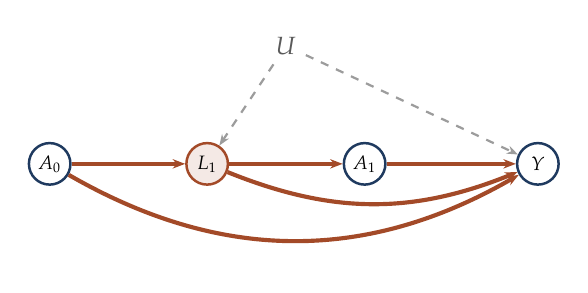
\begin{tikzpicture}[scale=1.0, every node/.style={font=\small}]
\node[knotenb] (a0) at (-3.0,0) {$A_0$};
\node[knotenr] (l1) at (-1.0,0) {$L_1$};
\node[knotenb] (a1) at (1.0,0) {$A_1$};
\node[knotenb] (y) at (3.2,0) {$Y$};
\node[grau] (u) at (0,1.5) {$U$};
\draw[kanted, -{Stealth[length=4.5pt]}] (a0)--(l1);
\draw[kanted, -{Stealth[length=4.5pt]}] (l1)--(a1);
\draw[kanted, -{Stealth[length=4.5pt]}] (a1)--(y);
\draw[kanted, -{Stealth[length=4.5pt]}] (a0) to[bend right=30] (y);
\draw[kanted, -{Stealth[length=4.5pt]}] (l1) to[bend right=22] (y);
\draw[grau!60, line width=0.8pt, dashed, -{Stealth[length=4pt]}] (u)--(l1);
\draw[grau!60, line width=0.8pt, dashed, -{Stealth[length=4pt]}] (u)--(y);
\end{tikzpicture}
\end{center}

\begin{center}
{\small
\renewcommand{\arraystretch}{1.5}
\begin{tabular}{@{}P{2.6cm}P{6.0cm}@{}}
\toprule
$L_1$ ist \textbf{Störgröße} & für die zweite Gabe --- es beeinflusst $A_1$ und $Y$. Man \kursiv{muss} anpassen.\\
$L_1$ ist \textbf{Mediator} & für die erste Gabe --- es liegt auf dem Weg $A_0 \to L_1 \to Y$. Man \kursiv{darf nicht} anpassen.\\
$L_1$ ist \textbf{Kollider} & von $A_0$ und $U$. Anpassen öffnet den Weg $A_0 \to L_1 \leftarrow U \to Y$.\\
\bottomrule
\end{tabular}}
\end{center}

\begin{center}
\begin{minipage}{0.9\textwidth}
\textbf{Dieselbe Größe muss zugleich angepasst und nicht angepasst werden. Kein Regressionsmodell kann das.}
\end{minipage}
\end{center}

\begin{center}
\begin{minipage}{0.88\textwidth}
\kursiv{\textbf{Das ist die Rückkopplung zwischen Behandlung und Störgröße}, und sie ist in der Medizin die Regel, sobald über die Zeit behandelt wird: Blutdruckmittel richten sich nach dem Blutdruck, Insulin nach dem Zucker, Beatmung nach den Blutgasen --- und alle diese Größen sind zugleich Folgen der bisherigen Behandlung.}
\end{minipage}
\end{center}
\end{merksatz}

\begin{merksatz}
\boxtitel{Der Leitfall gerechnet}
$400\,000$ Patienten; $A_0$ ausgelost, $A_1$ hängt von $L_1$ ab, $U$ unbeobachtet.

\begin{center}
{\small
\renewcommand{\arraystretch}{1.5}
\begin{tabular}{@{}P{3.4cm}P{2.4cm}P{2.0cm}@{}}
\toprule
\textbf{Auswertung} & \textbf{Effekt} & \\
\midrule
$Y$ auf $A_0$, roh & $-0{,}104$ & \\
an $L_1$ angepasst & $-0{,}068$ & \textcolor{akzent}{falsch}\\
\midrule
g-Formel, $\dops(1,1)$ gegen $\dops(0,0)$ & $\mathbf{-0{,}207}$ & \\
wahr & $\mathbf{-0{,}207}$ & \textcolor{gruen}{richtig}\\
\bottomrule
\end{tabular}}
\end{center}

\begin{center}
\begin{minipage}{0.9\textwidth}
\textbf{Beide üblichen Auswertungen verfehlen den wahren Effekt um die Hälfte bis zwei Drittel.}
\end{minipage}
\end{center}

\begin{center}
\begin{minipage}{0.88\textwidth}
\kursiv{Die rohe Rechnung unterschätzt, weil sie die zweite Gabe außer Acht lässt --- ein Patient, der am Tag $0$ nichts bekam, bekommt am Tag $1$ eher etwas. \textbf{Die angepasste Rechnung unterschätzt noch stärker, weil sie den Wirkweg über $L_1$ abschneidet} und zugleich den Kollider öffnet. Es gibt keine Anpassungsmenge, die hier hilft.}
\end{minipage}
\end{center}
\end{merksatz}

\section{Die g-Formel}

\begin{merksatz}
\boxtitel{Satz 12.1 --- Robins, 1986}
Unter Konsistenz, Positivität und der \Begriff{folgenweisen Unabhängigkeit} --- bei jedem Schritt ist die Behandlung, gegeben die bisherige Geschichte, so gut wie ausgelost --- gilt
\[ \Pr\bigl[Y \mid \dops(a_0,a_1)\bigr] = \sum_{\ell} \Pr[Y \mid a_0, \ell, a_1]\ \Pr[\ell \mid a_0] . \]

\schritt{Wie man sie liest}
\begin{center}
{\small
\renewcommand{\arraystretch}{1.52}
\begin{tabular}{@{}P{2.6cm}P{6.0cm}@{}}
\toprule
\textbf{Zweiter Faktor} & Wie sich $L_1$ entwickelt, \kursiv{wenn} man am Tag $0$ so behandelt --- der Mediatorweg bleibt erhalten.\\
\textbf{Erster Faktor} & Wie es weitergeht bei gegebenem $L_1$ --- dort wird angepasst, weil $L_1$ Störgröße der zweiten Gabe ist.\\
\bottomrule
\end{tabular}}
\end{center}

\begin{center}
\begin{minipage}{0.9\textwidth}
\textbf{$L_1$ wird angepasst, wo es Störgröße ist, und durchlaufen, wo es Mediator ist --- in derselben Formel.}
\end{minipage}
\end{center}

\schritt{Warum eine Regression das nicht kann}
\begin{center}
\begin{minipage}{0.88\textwidth}
\kursiv{Eine Regression hat für $L_1$ genau einen Koeffizienten --- entweder sie nimmt es auf oder nicht. \textbf{Die g-Formel dagegen behandelt $L_1$ zweimal verschieden}, weil sie die Zeit ernst nimmt: erst wird der Verlauf unter der Strategie erzeugt, dann der Ausgang. Man rechnet sie in der Praxis durch Simulation: Man zieht Patientenverläufe unter der gewünschten Strategie und mittelt den Ausgang.}
\end{minipage}
\end{center}
\end{merksatz}

\begin{merksatz}
\boxtitel{Der zweite Weg: Gewichten über die Zeit}
Statt zu summieren, kann man gewichten --- mit dem Produkt der Kehrwahrscheinlichkeiten über alle Zeitpunkte:
\[ w_i = \prod_{t} \frac{1}{\Pr\bigl[A_t = a_{it} \mid \text{Geschichte}\bigr]} \]

\begin{center}
\begin{minipage}{0.88\textwidth}
\kursiv{In der so gewichteten Bevölkerung hängt die Behandlung an keinem Zeitpunkt mehr vom Verlauf ab --- $L_1$ ist keine Störgröße mehr und darf weggelassen werden. \textbf{Das Modell, das man dann rechnet, heißt Randstrukturmodell}, weil es die Randverteilung der potentiellen Ergebnisse beschreibt statt der bedingten. Es ist das gebräuchlichste Verfahren für zeitabhängige Behandlungen.}
\end{minipage}
\end{center}
\end{merksatz}

\section{Der Bruchfall}

\begin{warnung}
\boxtitelr{Die Gewichte über die Zeit}
\begin{center}
{\small
\renewcommand{\arraystretch}{1.52}
\begin{tabular}{@{}P{2.8cm}P{5.8cm}@{}}
\toprule
\textbf{Produkt} & Zehn Zeitpunkte mit Wahrscheinlichkeit $0{,}7$ ergeben ein Gewicht von $1/0{,}7^{10} = 35$.\\
\textbf{Positivität} & Sie muss zu \kursiv{jedem} Zeitpunkt und für \kursiv{jede} Geschichte gelten --- eine viel stärkere Forderung als in Kapitel~2.\\
\textbf{Strategien} & \enquote{Immer behandeln} kommt in den Daten womöglich gar nicht vor.\\
\bottomrule
\end{tabular}}
\end{center}

\begin{center}
\begin{minipage}{0.88\textwidth}
\kursiv{Die dritte Zeile ist die härteste Grenze. \textbf{Je länger der Zeitraum, desto unwahrscheinlicher ist es, dass irgendein Patient einer festen Strategie über die ganze Zeit gefolgt ist} --- und ohne solche Patienten ist die Strategie nicht bewertbar. Man weicht deshalb auf \kursiv{dynamische} Strategien aus: \enquote{behandle, sobald das Laktat über $2$ steigt}, statt \enquote{behandle immer}. Solche Strategien bilden das ärztliche Handeln ohnehin besser ab.}
\end{minipage}
\end{center}
\end{warnung}

\section{Übungsaufgaben}

\begin{aufgabe}
\boxtitel{Aufgabe 12.1 --- Die g-Formel von Hand}
Gegeben:
\begin{center}
{\small
\renewcommand{\arraystretch}{1.48}
\begin{tabular}{@{}P{2.4cm}P{2.2cm}P{2.2cm}@{}}
\toprule
& $a_0 = 1$ & $a_0 = 0$\\
\midrule
$\Pr[L_1=1 \mid a_0]$ & $0{,}30$ & $0{,}60$\\
\bottomrule
\end{tabular}}
\end{center}
\begin{center}
{\small
\renewcommand{\arraystretch}{1.48}
\begin{tabular}{@{}P{3.4cm}P{2.0cm}P{2.0cm}@{}}
\toprule
$\Pr[Y=1 \mid a_0,\ell,a_1{=}1]$ & $\ell = 1$ & $\ell = 0$\\
\midrule
$a_0 = 1$ & $0{,}40$ & $0{,}10$\\
$a_0 = 0$ & $0{,}50$ & $0{,}15$\\
\bottomrule
\end{tabular}}
\end{center}
Berechnen Sie $\Pr[Y \mid \dops(1,1)]$ und $\Pr[Y \mid \dops(0,1)]$.

\loesung
\schritt{Schritt 1 --- Für $a_0 = 1$}
\[ 0{,}30\cdot0{,}40 + 0{,}70\cdot0{,}10 = 0{,}120 + 0{,}070 = 0{,}190 \]

\schritt{Schritt 2 --- Für $a_0 = 0$}
\[ 0{,}60\cdot0{,}50 + 0{,}40\cdot0{,}15 = 0{,}300 + 0{,}060 = 0{,}360 \]

\schritt{Schritt 3 --- Der Effekt der ersten Gabe}
\[ 0{,}190 - 0{,}360 = \mathbf{-0{,}170} \]

\schritt{Schritt 4 --- Und falsch gerechnet}
Passt man an $L_1$ an und mittelt über dessen \kursiv{Randverteilung} --- etwa $0{,}45$ ---, so erhält man
\[ \bigl[0{,}45\cdot0{,}40 + 0{,}55\cdot0{,}10\bigr] - \bigl[0{,}45\cdot0{,}50 + 0{,}55\cdot0{,}15\bigr] = 0{,}235 - 0{,}308 = -0{,}073 \]

\begin{center}
\begin{minipage}{0.9\textwidth}
\textbf{$-0{,}073$ statt $-0{,}170$: Weniger als die Hälfte.}
\end{minipage}
\end{center}

\begin{center}
\begin{minipage}{0.88\textwidth}
\kursiv{\textbf{Der Unterschied steckt allein in der Gewichtung von $L_1$}: Die g-Formel benutzt die Verteilung, die sich \kursiv{unter der jeweiligen Strategie} einstellt --- $0{,}30$ gegen $0{,}60$ ---, die falsche Rechnung eine feste. Genau darin liegt die Wirkung der ersten Gabe: Sie halbiert die Häufigkeit des Organversagens, und das ist der größte Teil ihres Nutzens.}
\end{minipage}
\end{center}
\end{aufgabe}

\begin{aufgabe}
\boxtitel{Aufgabe 12.2 --- Gewichte über zehn Tage}
Ein Patient erhält an zehn Tagen die Behandlung; die Wahrscheinlichkeit betrage je Tag $0{,}7$, bei zweien nur $0{,}3$. Welches Gewicht trägt er?

\loesung
\schritt{Schritt 1 --- Das Produkt}
\[ w = \frac{1}{0{,}7^{8}\cdot0{,}3^{2}} = \frac{1}{0{,}0576\cdot0{,}09} = \frac{1}{0{,}00518} = 193 \]

\schritt{Schritt 2 --- Zum Vergleich}
\begin{center}
{\small
\renewcommand{\arraystretch}{1.46}
\begin{tabular}{@{}P{3.4cm}P{2.4cm}@{}}
\toprule
\textbf{Verlauf} & \textbf{Gewicht}\\
\midrule
zehnmal $0{,}7$ & $35$\\
achtmal $0{,}7$, zweimal $0{,}3$ & $\mathbf{193}$\\
zehnmal $0{,}5$ & $1024$\\
\bottomrule
\end{tabular}}
\end{center}

\schritt{Schritt 3 --- Stabilisierte Gewichte}
Man multipliziert mit der Wahrscheinlichkeit derselben Folge \kursiv{ohne} Bedingung auf den Verlauf:
\[ w^{\text{stab}} = \prod_t \frac{\Pr[A_t = a_t \mid \text{bisherige Behandlung}]}{\Pr[A_t = a_t \mid \text{Geschichte}]} \]

\begin{center}
\begin{minipage}{0.88\textwidth}
\kursiv{Zähler und Nenner sind ähnlich groß, das Gewicht bleibt nahe bei eins --- im Beispiel etwa $2$ statt $193$. \textbf{Der Erwartungswert bleibt derselbe, die Streuung sinkt erheblich.} Das ist dasselbe Prinzip wie bei der Anpassung in der randomisierten Studie aus Kapitel~3: Man ändert nichts an der Unverzerrtheit und viel an der Genauigkeit.}
\end{minipage}
\end{center}
\end{aufgabe}

\begin{aufgabe}
\boxtitel{Aufgabe 12.3 --- Welche Strategie ist bewertbar?}
Über zehn Tage sei die Behandlungswahrscheinlichkeit je Tag $0{,}7$. Wie viele von $10\,000$ Patienten haben der Strategie \enquote{immer behandeln} vollständig entsprochen?

\loesung
\schritt{Schritt 1 --- Die Rechnung}
\[ 10\,000\cdot0{,}7^{10} = 10\,000\cdot0{,}0282 = 282 \]

\schritt{Schritt 2 --- Und \enquote{nie behandeln}}
\[ 10\,000\cdot0{,}3^{10} = 10\,000\cdot0{,}0000059 = \mathbf{0{,}06} \]

\begin{center}
\begin{minipage}{0.9\textwidth}
\textbf{Kein einziger Patient. Die Strategie \enquote{nie behandeln} ist aus diesen Daten nicht bewertbar.}
\end{minipage}
\end{center}

\schritt{Schritt 3 --- Was stattdessen geht}
\begin{center}
{\small
\renewcommand{\arraystretch}{1.5}
\begin{tabular}{@{}P{2.8cm}P{5.8cm}@{}}
\toprule
\textbf{Kürzerer Zeitraum} & Drei statt zehn Tage: $0{,}3^{3} = 2{,}7\,\%$, also $270$ Patienten.\\
\textbf{Dynamische Strategie} & \enquote{Behandle nur, wenn das Laktat über $2$ liegt} --- solche Verläufe kommen häufig vor.\\
\textbf{Modellieren} & Den Ausgang als Funktion der Behandlungsdauer modellieren, statt Strategien einzeln zu vergleichen.\\
\bottomrule
\end{tabular}}
\end{center}

\begin{center}
\begin{minipage}{0.88\textwidth}
\kursiv{\textbf{Die dritte Zeile tauscht Positivität gegen Modellannahme} --- man behauptet einen glatten Zusammenhang und kann dann auch Bereiche bewerten, in denen keine Daten liegen. Das ist ehrlich, solange man es sagt. Die zweite Zeile ist der bessere Weg: Sie stellt die Frage so, dass sie beantwortbar ist, und trifft zugleich besser, was Ärzte wirklich tun.}
\end{minipage}
\end{center}
\end{aufgabe}

\begin{geschichte}
\boxtitelg{Eine Arbeit über Arsen}
\Person{James Robins} veröffentlichte 1986 einen Aufsatz von $115$ Seiten über die Wirkung von Arsen auf Arbeiter einer Kupferhütte.

\begin{center}
\begin{minipage}{0.9\textwidth}
\kursiv{Das Problem: Wer krank wurde, verließ die belastete Abteilung --- die Belastung hing vom Gesundheitszustand ab, der wiederum von der bisherigen Belastung. \textbf{Robins entwickelte dafür die g-Formel}, und der Aufsatz gilt als einer der schwersten der Epidemiologie. Er wurde jahrelang kaum gelesen; erst die Behandlung der HIV-Infektion in den 1990er Jahren, bei der dasselbe Problem auftrat, machte das Verfahren bekannt.}
\end{minipage}
\end{center}

\schritt{Der gesunde Arbeiter}
\begin{center}
\begin{minipage}{0.9\textwidth}
\kursiv{Die Epidemiologie kannte das Problem als \enquote{Effekt des gesunden Arbeiters}: Beschäftigte sind gesünder als die Allgemeinbevölkerung, weil Kranke ausscheiden. \textbf{Man hatte es als Auswahlproblem gedeutet und mit Anpassung zu beheben versucht} --- und genau diese Anpassung machte es schlimmer, wie Abschnitt 12.1 zeigt.}
\end{minipage}
\end{center}
\end{geschichte}

\begin{forschung}
\boxtitelp{Über die Zeit heute}
\begin{center}
{\small
\renewcommand{\arraystretch}{1.45}
\begin{tabular}{@{}P{3.0cm}P{5.2cm}@{}}
\toprule
\textbf{Dynamische Strategien} & Regeln der Form \enquote{behandle, wenn}, statt fester Folgen.\\
\textbf{Intensivmedizin} & Beatmung, Flüssigkeit, Katecholamine --- alles rückgekoppelt.\\
\textbf{Bestärkendes Lernen} & Strategien aus Daten lernen statt sie zu vergleichen.\\
\bottomrule
\end{tabular}}
\end{center}

\schritt{Zur dritten Zeile}
\begin{center}
\begin{minipage}{0.88\textwidth}
\kursiv{Verfahren des bestärkenden Lernens suchen die beste Strategie, statt gegebene zu bewerten --- und stoßen dabei auf dieselbe Positivitätsgrenze, nur schärfer: \textbf{Die gefundene Strategie weicht gerade dort vom ärztlichen Handeln ab, wo es keine Daten gibt.} Eine vielbeachtete Arbeit von 2018 schlug für die Sepsisbehandlung Strategien vor, die Intensivmediziner für gefährlich hielten; die Nachprüfung zeigte, dass die Verfahren genau die datenarmen Bereiche bevorzugten.}
\end{minipage}
\end{center}
\end{forschung}

\begin{merksatz}
\boxtitel{Was Sie jetzt können}
\begin{center}
\renewcommand{\arraystretch}{1.5}
\begin{tabular}{@{}P{3.0cm}P{5.6cm}@{}}
\toprule
\textbf{Rückkopplung} & Störgröße und Mediator zugleich\\
\textbf{Satz 12.1} & g-Formel: erst Verlauf, dann Ausgang\\
\textbf{Gewichten} & Produkt über die Zeitpunkte\\
\textbf{Positivität} & zu jedem Zeitpunkt, für jede Geschichte\\
\textbf{Dynamisch} & die beantwortbare Frage stellen\\
\bottomrule
\end{tabular}
\end{center}

\begin{center}
\begin{minipage}{0.88\textwidth}
\kursiv{Die g-Formel durchläuft den Mediator, statt ihn zu sperren. Das nächste Kapitel fragt, wie viel Wirkung durch ihn läuft --- und stößt auf eine Annahme, die über zwei Welten zugleich spricht.}
\end{minipage}
\end{center}
\end{merksatz}

\chapter{Auf welchem Weg}

\section{Die Frage}

\begin{merksatz}
\boxtitel{Wirkt die frühe Gabe über das Organversagen?}
Der Gesamteffekt ist bekannt. Nun fragt man: Wie viel davon läuft über die Verhinderung des Organversagens, und wie viel auf anderem Wege --- über die Bakterienlast, über die Verweildauer, über anderes?

\begin{center}
{\small
\renewcommand{\arraystretch}{1.55}
\begin{tabular}{@{}P{2.6cm}P{6.0cm}@{}}
\toprule
\textbf{Gesamteffekt} & Wirkung von $X$ auf $Y$ auf allen Wegen.\\
\textbf{Indirekter Effekt} & Der Teil, der über $M$ läuft.\\
\textbf{Direkter Effekt} & Der Rest.\\
\bottomrule
\end{tabular}}
\end{center}

\begin{center}
\begin{minipage}{0.88\textwidth}
\kursiv{Die Frage ist nicht müßig. \textbf{Läuft die Wirkung ganz über $M$, so genügt es, $M$ zu behandeln} --- und man braucht die frühe Gabe nur, soweit sie $M$ verhindert. Läuft sie daran vorbei, so hilft die Behandlung von $M$ nicht. Das ist der Unterschied zwischen einer Ursachenkette und einem Bündel paralleler Wirkungen.}
\end{minipage}
\end{center}
\end{merksatz}

\begin{merksatz}
\boxtitel{Der lineare Fall}
Bei linearen Modellen ohne Wechselwirkung zerfällt der Effekt in ein Produkt und eine Summe:
\[ \text{gesamt} = \underbrace{c'}_{\text{direkt}} + \underbrace{a\cdot b}_{\text{indirekt}} \]
mit $a$: Wirkung von $X$ auf $M$; $b$: Wirkung von $M$ auf $Y$ bei festem $X$; $c'$: Wirkung von $X$ auf $Y$ bei festem $M$.

\schritt{Gerechnet}
$300\,000$ Patienten, $a = 0{,}6$, $b = 0{,}5$, $c' = 0{,}4$:

\begin{center}
{\small
\renewcommand{\arraystretch}{1.48}
\begin{tabular}{@{}P{2.6cm}P{2.2cm}P{2.4cm}@{}}
\toprule
\textbf{Größe} & \textbf{Schätzung} & \textbf{erwartet}\\
\midrule
gesamt & $0{,}697$ & $0{,}700$\\
direkt & $0{,}400$ & $0{,}400$\\
indirekt & $0{,}300$ & $0{,}300$\\
\midrule
Summe & $0{,}700$ & \checkmark\\
\bottomrule
\end{tabular}}
\end{center}

\[ \text{Anteil über den Mediator: } \frac{0{,}300}{0{,}697} = 43\,\% \]
\end{merksatz}

\section{Was der lineare Fall verbirgt}

\begin{merksatz}
\boxtitel{Kontrolliert und natürlich}
Sobald die Wirkung von $M$ davon abhängt, ob behandelt wurde, zerfällt der einfache Zusammenhang.

\begin{center}
{\small
\renewcommand{\arraystretch}{1.55}
\begin{tabular}{@{}P{3.0cm}P{5.6cm}@{}}
\toprule
\textbf{Kontrolliert direkt} & Effekt von $X$, wenn man $M$ bei allen auf denselben Wert \kursiv{zwingt}. Hängt davon ab, welchen.\\
\textbf{Natürlich direkt} & Effekt von $X$, wenn $M$ den Wert behält, den es \kursiv{ohne} Behandlung angenommen hätte.\\
\textbf{Natürlich indirekt} & Effekt der Verschiebung von $M$ --- bei festgehaltener Behandlung.\\
\bottomrule
\end{tabular}}
\end{center}

\begin{center}
\begin{minipage}{0.9\textwidth}
\textbf{Nur die natürlichen Effekte summieren sich zum Gesamteffekt.}
\end{minipage}
\end{center}

\schritt{Die Annahme, die dahintersteckt}
\begin{center}
\begin{minipage}{0.88\textwidth}
\kursiv{Die natürlich direkte Wirkung vergleicht den Ausgang bei Behandlung, aber mit dem Organversagen, das \kursiv{ohne} Behandlung eingetreten wäre. \textbf{Das ist eine Größe aus zwei verschiedenen Welten zugleich} --- behandelt in der einen Hinsicht, unbehandelt in der anderen. Sie ist in keinem Versuch herstellbar, auch nicht mit beliebigem Aufwand: Man kann einen Patienten nicht behandeln und ihm zugleich den Verlauf des Unbehandelten geben.}
\end{minipage}
\end{center}

\begin{center}
\begin{minipage}{0.88\textwidth}
\kursiv{\textbf{Die zugehörige Annahme heißt Kreuzwelt-Unabhängigkeit}, und sie ist grundsätzlich unprüfbar --- nicht bloß in der Praxis schwer zu prüfen, sondern aus logischen Gründen: Keine Beobachtung und kein Versuch können sie widerlegen. Das unterscheidet sie von allen anderen Annahmen dieses Bandes.}
\end{minipage}
\end{center}
\end{merksatz}

\section{Der Bruchfall}

\begin{warnung}
\boxtitelr{Drei Gründe für Vorsicht}
\begin{center}
{\small
\renewcommand{\arraystretch}{1.52}
\begin{tabular}{@{}P{2.8cm}P{5.8cm}@{}}
\toprule
\textbf{Störgrößen des Mediators} & Für die Zerlegung braucht man nicht nur $X$ unverzerrt, sondern auch $M \to Y$ --- also eine zweite, oft unbeachtete Anpassungsmenge.\\
\textbf{Folgen der Behandlung} & Ist eine Störgröße von $M \to Y$ selbst eine Folge von $X$, so sind die natürlichen Effekte nicht bestimmbar --- dieselbe Lage wie in Kapitel~12.\\
\textbf{Messfehler} & Ein ungenau gemessener Mediator verschiebt Anteile vom indirekten zum direkten Effekt.\\
\bottomrule
\end{tabular}}
\end{center}

\begin{center}
\begin{minipage}{0.88\textwidth}
\kursiv{Die dritte Zeile erklärt einen verbreiteten Befund: \textbf{Wer einen groben Mediator misst, findet einen großen \enquote{direkten} Effekt} --- und deutet ihn als eigenständigen Wirkweg, obwohl er nur den nicht erfassten Teil des indirekten Weges enthält. In der psychiatrischen Forschung, wo Mediatoren oft Fragebogenwerte sind, ist das die Regel.}
\end{minipage}
\end{center}
\end{warnung}

\section{Übungsaufgaben}

\begin{aufgabe}
\boxtitel{Aufgabe 13.1 --- Die Zerlegung rechnen}
$a = 0{,}6$, $b = 0{,}5$, $c' = 0{,}4$. Berechnen Sie die drei Effekte und den vermittelten Anteil. Was ändert sich, wenn $b$ auf $0{,}9$ steigt?

\loesung
\schritt{Schritt 1 --- Die Ausgangslage}
\[ \text{indirekt} = 0{,}6\cdot0{,}5 = 0{,}30, \qquad \text{gesamt} = 0{,}4+0{,}3 = 0{,}70 \]
\[ \text{Anteil} = 0{,}30/0{,}70 = 43\,\% \]

\schritt{Schritt 2 --- Mit $b = 0{,}9$}
\[ \text{indirekt} = 0{,}54, \qquad \text{gesamt} = 0{,}94, \qquad \text{Anteil} = 57\,\% \]

\schritt{Schritt 3 --- Die Tabelle}
\begin{center}
{\small
\renewcommand{\arraystretch}{1.46}
\begin{tabular}{@{}P{1.4cm}P{1.8cm}P{1.8cm}P{2.0cm}@{}}
\toprule
$b$ & \textbf{indirekt} & \textbf{gesamt} & \textbf{Anteil}\\
\midrule
$0{,}1$ & $0{,}06$ & $0{,}46$ & $13\,\%$\\
$0{,}5$ & $0{,}30$ & $0{,}70$ & $43\,\%$\\
$0{,}9$ & $0{,}54$ & $0{,}94$ & $57\,\%$\\
\bottomrule
\end{tabular}}
\end{center}

\begin{center}
\begin{minipage}{0.88\textwidth}
\kursiv{\textbf{Der vermittelte Anteil hängt vom Nenner ab und ist deshalb schlecht zu vergleichen.} Zwei Studien mit demselben indirekten Effekt berichten verschiedene Anteile, wenn ihre Gesamteffekte sich unterscheiden --- etwa weil die Bevölkerungen verschieden sind. Man berichtet daher besser die absoluten Effekte.}
\end{minipage}
\end{center}
\end{aufgabe}

\begin{aufgabe}
\boxtitel{Aufgabe 13.2 --- Wenn der Mediator ungenau gemessen ist}
Der wahre Mediator werde nur mit einer Korrelation von $0{,}7$ erfasst. Wie verschiebt sich die Zerlegung?

\loesung
\schritt{Schritt 1 --- Der Mechanismus}
Bei klassischem Messfehler wird der Koeffizient $b$ um den Faktor der Zuverlässigkeit gedämpft:
\[ b_{\text{gemessen}} \approx 0{,}7^{2}\cdot b = 0{,}49\,b \]

\schritt{Schritt 2 --- Die Folge}
\begin{center}
{\small
\renewcommand{\arraystretch}{1.46}
\begin{tabular}{@{}P{2.4cm}P{2.0cm}P{2.0cm}@{}}
\toprule
& \textbf{wahr} & \textbf{gemessen}\\
\midrule
indirekt & $0{,}30$ & $0{,}15$\\
direkt & $0{,}40$ & $0{,}55$\\
gesamt & $0{,}70$ & $0{,}70$\\
Anteil & $43\,\%$ & $\mathbf{21\,\%}$\\
\bottomrule
\end{tabular}}
\end{center}

\begin{center}
\begin{minipage}{0.9\textwidth}
\textbf{Der Gesamteffekt bleibt richtig; die Aufteilung verschiebt sich um die Hälfte.}
\end{minipage}
\end{center}

\begin{center}
\begin{minipage}{0.88\textwidth}
\kursiv{\textbf{Was der Mediator nicht erfasst, erscheint als direkter Effekt} --- der direkte Effekt ist eine Restgröße und erbt jeden Fehler. Deshalb ist der Satz \enquote{die Wirkung läuft nur teilweise über $M$} fast nie belastbar, solange die Messgenauigkeit von $M$ nicht bekannt ist.}
\end{minipage}
\end{center}
\end{aufgabe}

\begin{aufgabe}
\boxtitel{Aufgabe 13.3 --- Zwei Welten zugleich}
Warum lässt sich der natürlich direkte Effekt nicht durch einen Versuch bestimmen?

\loesung
\schritt{Schritt 1 --- Was er verlangt}
\[ \mathbb{E}\bigl[Y\bigl(1,\ M(0)\bigr)\bigr] - \mathbb{E}\bigl[Y\bigl(0,\ M(0)\bigr)\bigr] \]
--- der erste Ausdruck beschreibt einen Patienten, der behandelt wird, dessen Organversagen aber dem Verlauf ohne Behandlung folgt.

\schritt{Schritt 2 --- Warum das kein Versuch leisten kann}
\begin{center}
{\small
\renewcommand{\arraystretch}{1.5}
\begin{tabular}{@{}P{2.8cm}P{5.8cm}@{}}
\toprule
\textbf{$M$ zwingen} & ergibt den \kursiv{kontrollierten} Effekt --- dabei wird $M$ auf einen festen Wert gesetzt, nicht auf den individuellen Wert ohne Behandlung.\\
\textbf{$M(0)$ beobachten} & geht nur bei Unbehandelten --- dann kann man nicht zugleich behandeln.\\
\bottomrule
\end{tabular}}
\end{center}

\begin{center}
\begin{minipage}{0.9\textwidth}
\textbf{Die Größe bezieht sich auf keinen möglichen Versuch. Sie ist eine Erfindung des Formalismus --- aber eine nützliche.}
\end{minipage}
\end{center}

\schritt{Schritt 3 --- Wozu sie dann gut ist}
\begin{center}
\begin{minipage}{0.88\textwidth}
\kursiv{\textbf{Sie beantwortet die Frage nach dem \kursiv{Mechanismus}, nicht nach einer Handlung.} Wer wissen will, ob eine Behandlung wirkt, braucht sie nicht. Wer verstehen will, warum, braucht etwas in dieser Art --- und muss dafür eine Annahme hinnehmen, die niemand prüfen kann. Der kontrollierte direkte Effekt ist dagegen prüfbar und beantwortet eine andere, oft ebenso brauchbare Frage: Was bringt die Behandlung, wenn man $M$ ohnehin behandelt?}
\end{minipage}
\end{center}
\end{aufgabe}

\begin{geschichte}
\boxtitelg{Von der Psychologie zur Mathematik}
\Person{Reuben Baron} und \Person{David Kenny} veröffentlichten 1986 ein Verfahren zur Mediationsanalyse, das aus drei Regressionen bestand.

\begin{center}
\begin{minipage}{0.9\textwidth}
\kursiv{Der Aufsatz erschien in einer psychologischen Zeitschrift und wurde zu einem der meistzitierten Texte der Sozialwissenschaften überhaupt --- über hunderttausend Nennungen. \textbf{Sein Verfahren ist unter Wechselwirkungen falsch} und setzt stillschweigend voraus, dass für den Mediator dieselben Störgrößen genügen wie für die Behandlung.}
\end{minipage}
\end{center}

\schritt{Die Berichtigung}
\begin{center}
\begin{minipage}{0.9\textwidth}
\kursiv{\Person{Judea Pearl} und \Person{Jacques Robins} klärten in den 1990er Jahren, welche Größen überhaupt gemeint sind, und führten die natürlichen Effekte ein. \textbf{\Person{Tyler VanderWeele} machte daraus ab 2009 ein Lehrgebäude für die Epidemiologie.} Die alte Dreiregressionsmethode wird dennoch weiter benutzt --- ein Beispiel dafür, wie lange ein bequemes Verfahren überlebt, nachdem seine Grenzen bekannt sind.}
\end{minipage}
\end{center}
\end{geschichte}

\begin{forschung}
\boxtitelp{Mechanismen heute}
\begin{center}
{\small
\renewcommand{\arraystretch}{1.45}
\begin{tabular}{@{}P{3.0cm}P{5.2cm}@{}}
\toprule
\textbf{Trennbare Effekte} & Wirkungen so zerlegen, dass jeder Teil einem möglichen Eingriff entspricht.\\
\textbf{Mehrere Mediatoren} & Wege, die sich gegenseitig beeinflussen.\\
\textbf{Empfindlichkeit} & Wie stark die Kreuzwelt-Annahme verletzt sein dürfte.\\
\bottomrule
\end{tabular}}
\end{center}

\schritt{Zur ersten Zeile}
\begin{center}
\begin{minipage}{0.88\textwidth}
\kursiv{Statt eine Behandlung nachträglich in Wege zu zerlegen, denkt man sie sich in Bestandteile zerlegt, die getrennt gegeben werden könnten --- etwa ein Antibiotikum, das die Bakterien tötet, und eines, das zusätzlich entzündungshemmend wirkt. \textbf{Jeder Teileffekt entspricht dann einem denkbaren Versuch}, und die Kreuzwelt-Annahme entfällt. Der Preis ist, dass man die Zerlegung inhaltlich begründen muss --- was die Frage vom Formalismus zurück in die Pharmakologie verlagert.}
\end{minipage}
\end{center}
\end{forschung}

\begin{merksatz}
\boxtitel{Was Sie jetzt können}
\begin{center}
\renewcommand{\arraystretch}{1.5}
\begin{tabular}{@{}P{3.0cm}P{5.6cm}@{}}
\toprule
\textbf{Linear} & gesamt $= c' + ab$\\
\textbf{Kontrolliert} & $M$ auf einen Wert zwingen\\
\textbf{Natürlich} & $M$ auf seinen Wert ohne Behandlung\\
\textbf{Kreuzwelt} & grundsätzlich unprüfbar\\
\textbf{Messfehler} & verschiebt indirekt nach direkt\\
\bottomrule
\end{tabular}
\end{center}

\begin{center}
\begin{minipage}{0.88\textwidth}
\kursiv{Bisher ging es um Durchschnitte über alle. Das nächste Kapitel fragt nach dem einzelnen Patienten --- und findet, dass die Antwort für jeden anders ausfällt.}
\end{minipage}
\end{center}
\end{merksatz}

\chapter{Für wen es wirkt}

\section{Der Durchschnitt verbirgt}

\begin{merksatz}
\boxtitel{Ein Effekt, vier Zahlen}
$300\,000$ Patienten, Behandlung ausgelost. Der Effekt hängt vom Alter ab: bei den Jüngsten $-0{,}20$, bei den Ältesten $0$.

\begin{center}
{\small
\renewcommand{\arraystretch}{1.48}
\begin{tabular}{@{}P{2.2cm}P{2.4cm}P{2.4cm}@{}}
\toprule
\textbf{Alter} & \textbf{geschätzt} & \textbf{wahr}\\
\midrule
$40$--$55$ & $-0{,}171$ & $-0{,}170$\\
$55$--$70$ & $-0{,}107$ & $-0{,}110$\\
$70$--$85$ & $-0{,}053$ & $-0{,}050$\\
$85$--$90$ & $-0{,}029$ & $-0{,}010$\\
\midrule
\textbf{alle} & \textbf{$-0{,}100$} & $-0{,}100$\\
\bottomrule
\end{tabular}}
\end{center}

\begin{center}
\begin{minipage}{0.9\textwidth}
\textbf{Der Durchschnittseffekt von zehn Punkten gilt für niemanden: Die Jungen gewinnen doppelt so viel, die Alten nichts.}
\end{minipage}
\end{center}

\begin{center}
\begin{minipage}{0.88\textwidth}
\kursiv{\textbf{Das ist die zweite Warnung des Vorworts in Zahlen.} Ein Durchschnittseffekt ist ein Mittelwert über eine Bevölkerung --- und wie jeder Mittelwert sagt er nichts über die Streuung. Er kann sogar positiv sein, während die Behandlung der Hälfte schadet; das sieht man ihm nicht an.}
\end{minipage}
\end{center}
\end{merksatz}

\begin{merksatz}
\boxtitel{Was man schätzen will}
\[ \tau(\vek z) = \mathbb{E}\bigl[Y(1) - Y(0) \ \big|\ Z = \vek z\bigr] \]
--- der Effekt bei Patienten mit den Merkmalen $\vek z$.

\begin{center}
{\small
\renewcommand{\arraystretch}{1.52}
\begin{tabular}{@{}P{2.6cm}P{6.0cm}@{}}
\toprule
\textbf{Nicht} & der Effekt \kursiv{dieses} Patienten --- der bleibt nach Satz 2.2 unbekannt.\\
\textbf{Sondern} & der Durchschnitt über alle, die ihm in den gemessenen Merkmalen gleichen.\\
\bottomrule
\end{tabular}}
\end{center}

\begin{center}
\begin{minipage}{0.88\textwidth}
\kursiv{\textbf{Je mehr Merkmale, desto näher kommt man dem Einzelnen --- und desto größer wird die Streuung}, denn in jeder Zelle bleiben weniger Patienten. Es ist der Zielkonflikt aus Band 22, Kapitel~2, nun auf eine Differenz angewandt: Man schätzt nicht einen Ausgang, sondern den Unterschied zweier Ausgänge, und Differenzen sind erheblich unschärfer als ihre Bestandteile.}
\end{minipage}
\end{center}
\end{merksatz}

\section{Wie man es schätzt}

\begin{merksatz}
\boxtitel{Drei Wege}
\begin{center}
{\small
\renewcommand{\arraystretch}{1.55}
\begin{tabular}{@{}P{2.8cm}P{5.8cm}@{}}
\toprule
\textbf{Untergruppen} & Vorher festgelegte Gruppen getrennt auswerten. Ehrlich, aber grob und schnell erschöpft.\\
\textbf{Wechselwirkung} & Ein Term $X\cdot Z$ im Modell. Unterstellt eine Form.\\
\textbf{Kausale Wälder} & Bäume, die nicht nach dem Ausgang, sondern nach dem \kursiv{Unterschied} der Ausgänge teilen --- Band 22, Kapitel~9.\\
\bottomrule
\end{tabular}}
\end{center}

\begin{center}
\begin{minipage}{0.88\textwidth}
\kursiv{Ein kausaler Wald sucht die Aufteilung, bei der sich die geschätzten Effekte der beiden Gruppen am stärksten unterscheiden. \textbf{Der entscheidende Kunstgriff heißt Ehrlichkeit}: Eine Hälfte der Daten bestimmt, wo geteilt wird, die andere schätzt in den entstandenen Blättern. Ohne diese Trennung findet der Wald Unterschiede, die er selbst erzeugt hat --- das Leck aus Band 22, Kapitel~3, in kausaler Gestalt.}
\end{minipage}
\end{center}
\end{merksatz}

\section{Der Bruchfall}

\begin{warnung}
\boxtitelr{Untergruppen, die keine sind}
\begin{center}
{\small
\renewcommand{\arraystretch}{1.52}
\begin{tabular}{@{}P{2.8cm}P{5.8cm}@{}}
\toprule
\textbf{Multiples Testen} & Zwanzig Untergruppen ergeben bei reinem Zufall eine \enquote{bedeutsame}.\\
\textbf{Skalenabhängig} & Ein Effekt kann auf der Differenzskala schwanken und auf der Verhältnisskala konstant sein --- und umgekehrt.\\
\textbf{Streuung} & Der Effekt in einer Untergruppe wird aus einer Differenz zweier Differenzen geschätzt --- vierfache Fallzahl für gleiche Genauigkeit.\\
\bottomrule
\end{tabular}}
\end{center}

\schritt{Zur zweiten Zeile}
\begin{center}
\begin{minipage}{0.88\textwidth}
\kursiv{Senkt eine Behandlung das Risiko überall um $20$ Prozent \kursiv{relativ}, so beträgt die absolute Senkung bei einem Grundrisiko von $40$ Prozent acht Punkte, bei zehn Prozent nur zwei. \textbf{Auf der Verhältnisskala gibt es dann keine Heterogenität, auf der Differenzskala erhebliche} --- und beide Beschreibungen sind richtig. Für die Behandlungsentscheidung zählt die absolute, denn sie sagt, wie viele Patienten man behandeln muss.}
\end{minipage}
\end{center}

\begin{center}
\begin{minipage}{0.88\textwidth}
\kursiv{\textbf{Daraus folgt: Die wichtigste Quelle von Heterogenität ist das Grundrisiko}, nicht eine besondere Empfindlichkeit. Wer wissen will, wem eine Behandlung am meisten nützt, schätzt zuerst das Risiko ohne Behandlung --- das ist eine Vorhersageaufgabe im Sinne von Band 22 --- und wendet darauf den relativen Effekt an. Dieses zweistufige Vorgehen ist robuster als die unmittelbare Schätzung von $\tau(\vek z)$.}
\end{minipage}
\end{center}
\end{warnung}

\section{Übungsaufgaben}

\begin{aufgabe}
\boxtitel{Aufgabe 14.1 --- Wie viele Patienten je Untergruppe?}
Der Gesamteffekt beträgt $-0{,}10$ bei einem Grundrisiko von $0{,}30$. Wie viele Patienten braucht man, um einen Unterschied von $0{,}10$ zwischen zwei Untergruppen nachzuweisen?

\loesung
\schritt{Schritt 1 --- Der Haupteffekt}
Nach Kapitel~3:
\[ n = \frac{(1{,}96+0{,}84)^{2}\,\bigl[0{,}30\cdot0{,}70 + 0{,}20\cdot0{,}80\bigr]}{0{,}10^{2}} = \frac{7{,}85\cdot0{,}37}{0{,}01} = 291 \ \text{je Gruppe} \]

\schritt{Schritt 2 --- Der Unterschied zweier Effekte}
Er ist eine Differenz zweier Differenzen; seine Varianz ist die Summe von vier Varianzen statt zweier:
\[ n = 4\cdot291 = 1164 \ \text{je Gruppe} \]

\begin{center}
{\small
\renewcommand{\arraystretch}{1.48}
\begin{tabular}{@{}P{3.0cm}P{2.2cm}P{2.4cm}@{}}
\toprule
\textbf{Frage} & \textbf{je Gruppe} & \textbf{gesamt}\\
\midrule
Wirkt es? & $291$ & $582$\\
Wirkt es verschieden? & $1164$ & $\mathbf{4656}$\\
\bottomrule
\end{tabular}}
\end{center}

\begin{center}
\begin{minipage}{0.9\textwidth}
\textbf{Achtmal so viele Patienten für die Frage nach dem Unterschied.}
\end{minipage}
\end{center}

\begin{center}
\begin{minipage}{0.88\textwidth}
\kursiv{\textbf{Deshalb sind Untergruppenbefunde aus Studien, die für den Haupteffekt geplant wurden, fast immer unzuverlässig} --- sie haben für diese Frage eine Trennschärfe von vielleicht zwanzig Prozent. Ein \enquote{kein Effekt in dieser Untergruppe} heißt dann meist nur: zu wenige Patienten.}
\end{minipage}
\end{center}
\end{aufgabe}

\begin{aufgabe}
\boxtitel{Aufgabe 14.2 --- Behandeln oder nicht?}
Mit dem Effektverlauf aus Abschnitt 14.1: Welche Politik ist die beste, wenn die Behandlung Nebenwirkungen im Wert von $0{,}03$ Punkten hat?

\loesung
\schritt{Schritt 1 --- Die Schwelle}
Behandeln lohnt, solange $\tau(\text{Alter}) < -0{,}03$:
\[ -0{,}20 + 0{,}004\,(\text{Alter}-40) < -0{,}03 \quad\Longrightarrow\quad \text{Alter} < 82{,}5 \]

\schritt{Schritt 2 --- Der Gewinn der drei Politiken}
\begin{center}
{\small
\renewcommand{\arraystretch}{1.48}
\begin{tabular}{@{}P{2.8cm}P{2.4cm}P{2.4cm}@{}}
\toprule
\textbf{Politik} & \textbf{Nutzen} & \\
\midrule
niemanden & $0$ & \\
alle & $-0{,}100+0{,}030 = -0{,}070$ & \\
unter $82{,}5$ & $\mathbf{-0{,}072}$ & \textcolor{gruen}{beste}\\
\bottomrule
\end{tabular}}
\end{center}

\kursiv{Zur letzten Zeile:} $85$ Prozent der Patienten sind jünger als $82{,}5$; ihr mittlerer Effekt beträgt $-0{,}115$, abzüglich $0{,}03$ ergibt $0{,}85\cdot(-0{,}085) = -0{,}072$; bei den Älteren geht nichts verloren, weil sie unbehandelt bleiben.

\schritt{Schritt 3 --- Die Einordnung}
\begin{center}
\begin{minipage}{0.88\textwidth}
\kursiv{\textbf{Der Gewinn durch gezieltes Behandeln ist hier klein} --- zwei Tausendstel gegenüber \enquote{alle behandeln}. Das ist typisch: Solange der Effekt überall dasselbe Vorzeichen hat, bringt die Auswahl wenig. Lohnend wird sie erst, wenn die Behandlung bei einem Teil der Patienten \kursiv{schadet} --- und dann hängt alles daran, ob man diesen Teil zuverlässig erkennt.}
\end{minipage}
\end{center}

\schritt{Schritt 4 --- Und die Unsicherheit}
\begin{center}
\begin{minipage}{0.88\textwidth}
\kursiv{Die geschätzte Schwelle von $82{,}5$ Jahren hat selbst ein Vertrauensintervall, und zwar ein breites --- in Aufgabe 14.1 wurde sichtbar, wie teuer die Schätzung von Unterschieden ist. \textbf{Eine Politik, die an einer ungenau geschätzten Schwelle hängt, kann schlechter sein als gar keine Auswahl.} Man vergleicht deshalb Politiken nicht am geschätzten Optimum, sondern an ihrem Nutzen unter Unsicherheit.}
\end{minipage}
\end{center}
\end{aufgabe}

\begin{aufgabe}
\boxtitel{Aufgabe 14.3 --- Skala und Heterogenität}
Eine Behandlung senkt das Risiko überall um $25$ Prozent relativ. Ist der Effekt heterogen?

\loesung
\schritt{Schritt 1 --- Die absoluten Effekte}
\begin{center}
{\small
\renewcommand{\arraystretch}{1.46}
\begin{tabular}{@{}P{2.2cm}P{2.0cm}P{2.0cm}P{2.2cm}@{}}
\toprule
\textbf{Grundrisiko} & \textbf{mit} & \textbf{Differenz} & \textbf{Zahl nötig}\\
\midrule
$0{,}40$ & $0{,}30$ & $-0{,}10$ & $10$\\
$0{,}20$ & $0{,}15$ & $-0{,}05$ & $20$\\
$0{,}05$ & $0{,}0375$ & $-0{,}0125$ & $80$\\
\bottomrule
\end{tabular}}
\end{center}
\kursiv{\enquote{Zahl nötig} ist die Zahl der Behandelten je verhindertem Ereignis.}

\schritt{Schritt 2 --- Die Antwort}
\begin{center}
\begin{minipage}{0.9\textwidth}
\textbf{Auf der Verhältnisskala nein, auf der Differenzskala ja --- achtfach.}
\end{minipage}
\end{center}

\schritt{Schritt 3 --- Was für die Praxis zählt}
\begin{center}
\begin{minipage}{0.88\textwidth}
\kursiv{Die letzte Spalte entscheidet über den Einsatz: \textbf{Bei einem Grundrisiko von fünf Prozent muss man achtzig Patienten behandeln, um ein Ereignis zu verhindern} --- bei vierzig Prozent nur zehn. Ist die Behandlung teuer oder belastend, so lohnt sie im einen Fall und im anderen nicht, obwohl sie \enquote{gleich gut wirkt}.}
\end{minipage}
\end{center}

\schritt{Schritt 4 --- Die Folgerung für Leitlinien}
\begin{center}
\begin{minipage}{0.88\textwidth}
\kursiv{\textbf{Eine Leitlinie sollte den relativen Effekt aus Studien mit dem individuellen Grundrisiko aus einem Vorhersagemodell verbinden} --- statt Untergruppen nach Alter oder Geschlecht zu bilden. Damit treffen sich Band 22 und dieser Band an der Stelle, auf die es klinisch ankommt: Die Vorhersage sagt, wie gefährdet jemand ist; der kausale Schluss sagt, was die Behandlung daran ändert.}
\end{minipage}
\end{center}
\end{aufgabe}

\begin{geschichte}
\boxtitelg{Die Untergruppe der Zwillinge}
In einer großen Herzstudie der 1980er Jahre wurde die Wirkung von Aspirin nach Sternzeichen ausgewertet.

\begin{center}
\begin{minipage}{0.9\textwidth}
\kursiv{Bei Zwillingen und Waagen zeigte sich kein Nutzen, in allen anderen Zeichen ein deutlicher. \textbf{Die Verfasser druckten das Ergebnis ausdrücklich ab, um zu zeigen, wie wenig Untergruppenanalysen wert sind.} Der Scherz wird seither in jeder Methodenvorlesung erzählt --- und die Praxis der Untergruppenauswertung hat er nicht beendet.}
\end{minipage}
\end{center}

\schritt{Und ein ernster Fall}
\begin{center}
\begin{minipage}{0.9\textwidth}
\kursiv{Mehrfach wurden Medikamente aufgrund von Untergruppenbefunden gezielt eingesetzt und später widerlegt --- oder umgekehrt Patientengruppen ausgeschlossen, denen das Mittel geholfen hätte. \textbf{Die Zulassungsbehörden verlangen deshalb heute, Untergruppen vorab zu benennen} und den Wechselwirkungsterm zu prüfen, statt Gruppen getrennt auszuwerten.}
\end{minipage}
\end{center}
\end{geschichte}

\begin{forschung}
\boxtitelp{Einzelfall heute}
\begin{center}
{\small
\renewcommand{\arraystretch}{1.45}
\begin{tabular}{@{}P{3.0cm}P{5.2cm}@{}}
\toprule
\textbf{Kausale Wälder} & Heterogenität ohne vorgegebene Form, mit Vertrauensintervallen.\\
\textbf{Politiklernen} & Behandlungsregeln, die den Nutzen unter Nebenbedingungen maximieren.\\
\textbf{Risikobasierte Auswertung} & Studien nach vorhergesagtem Grundrisiko schichten.\\
\bottomrule
\end{tabular}}
\end{center}

\schritt{Zur dritten Zeile}
\begin{center}
\begin{minipage}{0.88\textwidth}
\kursiv{Man teilt die Studienteilnehmer nach ihrem \kursiv{vorhergesagten} Risiko in Viertel und berichtet den absoluten Effekt je Viertel. \textbf{Das ist eine einzige, vorab festgelegte Untergruppenbildung statt vieler} --- und sie trifft die klinisch wichtigste Quelle von Heterogenität. Mehrere Fachgesellschaften empfehlen dieses Vorgehen inzwischen als Standard.}
\end{minipage}
\end{center}
\end{forschung}

\begin{merksatz}
\boxtitel{Was Sie jetzt können}
\begin{center}
\renewcommand{\arraystretch}{1.5}
\begin{tabular}{@{}P{3.0cm}P{5.6cm}@{}}
\toprule
\textbf{$\tau(\vek z)$} & Durchschnitt über Gleichartige, nicht der Einzelne\\
\textbf{Drei Wege} & Untergruppen, Wechselwirkung, kausale Wälder\\
\textbf{Ehrlichkeit} & teilen und schätzen getrennt\\
\textbf{Achtfach} & Fallzahl für Unterschiede\\
\textbf{Skala} & Heterogenität hängt an ihr\\
\bottomrule
\end{tabular}
\end{center}

\begin{center}
\begin{minipage}{0.88\textwidth}
\kursiv{Damit endet Teil~V. Das letzte Kapitel zieht Bilanz --- und kehrt ein letztes Mal zur Tabelle aus Kapitel~1 zurück.}
\end{minipage}
\end{center}
\end{merksatz}

\part{Aktueller Stand}

\chapter{Woran es liegt}

\section{Die Tabelle aus Kapitel 1, ein letztes Mal}

\begin{merksatz}
\boxtitel{Was inzwischen dazugehört}
Am Anfang stand eine Tabelle, die zeigte, dass früh behandelte Patienten häufiger starben.

\begin{center}
{\small
\renewcommand{\arraystretch}{1.5}
\begin{tabular}{@{}P{1.2cm}P{3.6cm}P{3.6cm}@{}}
\toprule
\textbf{Kap.} & \textbf{Frage} & \textbf{Antwort}\\
\midrule
$1$ & Was zeigt die Tabelle? & Nichts Kausales.\\
$2$ & Was will man wissen? & $\mathbb{E}[Y(1)-Y(0)]$.\\
$3$ & Wie käme man hin? & Auslosen.\\
$4$--$6$ & Und ohne Los? & Hinterwege sperren.\\
$7$--$8$ & Womit? & Neigung, Gewichte.\\
$9$--$11$ & Wenn das nicht geht? & Instrument, Sprung, Nachbildung.\\
$12$--$14$ & Über die Zeit, für wen? & g-Formel, $\tau(\vek z)$.\\
\bottomrule
\end{tabular}}
\end{center}

\begin{center}
\begin{minipage}{0.9\textwidth}
\textbf{Keine dieser Antworten steckt in den Daten. Sie alle bestehen darin, die richtige Annahme zu benennen und ihre Folgen auszurechnen.}
\end{minipage}
\end{center}
\end{merksatz}

\section{Vier Muster}

\begin{merksatz}
\boxtitel{Muster 1 --- die Daten entscheiden nicht}
\begin{center}
{\small
\renewcommand{\arraystretch}{1.48}
\begin{tabular}{@{}P{1.4cm}P{7.0cm}@{}}
\toprule
$1$ & Satz 1.2: Dieselbe Tabelle, Effekt $+0{,}60$ oder null.\\
$4$ & Drei Graphen sind ununterscheidbar; nur der Kollider verrät sich.\\
$6$ & Manchmal gibt es gar keine zulässige Anpassungsmenge.\\
$13$ & Die Kreuzwelt-Annahme ist grundsätzlich unprüfbar.\\
\bottomrule
\end{tabular}}
\end{center}

\begin{center}
\begin{minipage}{0.88\textwidth}
\kursiv{\textbf{Das ist keine Schwäche des Faches, sondern sein wichtigster Beitrag.} Vor diesen Verfahren rechnete man Regressionen und sprach von \enquote{Einfluss}; die Annahmen blieben unausgesprochen und damit unbestreitbar. Wer heute einen Graphen zeichnet, legt sie offen --- und jeder Fachkollege kann einen Pfeil bestreiten.}
\end{minipage}
\end{center}
\end{merksatz}

\begin{merksatz}
\boxtitel{Muster 2 --- mehr anpassen ist nicht besser}
\begin{center}
{\small
\renewcommand{\arraystretch}{1.48}
\begin{tabular}{@{}P{1.4cm}P{7.0cm}@{}}
\toprule
$5$ & Mediator: Effekt von $0{,}72$ auf $0{,}004$.\\
$5$ & Kollider: aus null wird $-0{,}39$.\\
$5$ & Instrument: Verzerrung verdoppelt.\\
$12$ & Dieselbe Größe muss zugleich angepasst und durchlaufen werden.\\
\bottomrule
\end{tabular}}
\end{center}

\begin{center}
\begin{minipage}{0.88\textwidth}
\kursiv{\textbf{In jedem dieser Fälle sieht das falsche Modell besser aus als das richtige} --- es erklärt mehr Streuung, hat engere Intervalle und bestandene Gütemaße. Kein Auswahlverfahren aus Band 22 findet den Fehler, weil er nicht in den Daten steckt.}
\end{minipage}
\end{center}
\end{merksatz}

\begin{merksatz}
\boxtitel{Muster 3 --- der Entwurf schlägt das Verfahren}
\begin{center}
{\small
\renewcommand{\arraystretch}{1.48}
\begin{tabular}{@{}P{1.4cm}P{7.0cm}@{}}
\toprule
$3$ & Nach Behandlung statt nach Zuteilung: fast doppelter Effekt.\\
$11$ & Unsterbliche Zeit: $73$ Prozent Gewinn aus nichts.\\
$11$ & Die Hormonstudien widersprachen sich wegen des Beginns, nicht wegen der Störgrößen.\\
$14$ & Untergruppen brauchen die achtfache Fallzahl.\\
\bottomrule
\end{tabular}}
\end{center}

\begin{center}
\begin{minipage}{0.88\textwidth}
\kursiv{\textbf{Die größten Fehler dieses Bandes sind Entwurfsfehler, keine Rechenfehler} --- und sie sind vermeidbar. Das ist dieselbe Lehre wie in Band 22, Kapitel~3, wo die Prüfung wichtiger war als das Verfahren. Wer die sieben Zeilen der Zielstudie ausfüllt, bevor er rechnet, hat mehr gewonnen als durch jede Verfeinerung des Schätzers.}
\end{minipage}
\end{center}
\end{merksatz}

\begin{merksatz}
\boxtitel{Muster 4 --- jede Zahl gilt für eine Bevölkerung}
\begin{center}
{\small
\renewcommand{\arraystretch}{1.48}
\begin{tabular}{@{}P{1.4cm}P{7.0cm}@{}}
\toprule
$2$ & $\tau$ und $\tau_{\text{beh}}$: $-0{,}375$ gegen $-0{,}250$.\\
$9$ & Der Instrumentschätzer gilt für die Befolger --- die niemand benennen kann.\\
$10$ & Der Sprung gilt an der Schwelle.\\
$14$ & Der Durchschnitt von $-0{,}10$ gilt für niemanden.\\
\bottomrule
\end{tabular}}
\end{center}

\begin{center}
\begin{minipage}{0.88\textwidth}
\kursiv{\textbf{Ein kausaler Effekt ohne Angabe der Bevölkerung ist unvollständig} --- so unvollständig wie ein Mittelwert ohne Angabe, worüber gemittelt wurde. Die Verfahren dieses Bandes unterscheiden sich weniger in ihrer Güte als in der Frage, die sie beantworten.}
\end{minipage}
\end{center}
\end{merksatz}

\section{Was offen ist}

\begin{merksatz}
\boxtitel{Vier Fragen}
\begin{center}
{\small
\renewcommand{\arraystretch}{1.55}
\begin{tabular}{@{}P{3.0cm}P{5.6cm}@{}}
\toprule
\textbf{Übertragung} & Wann gilt ein Effekt in einer anderen Klinik? Kapitel~6 gibt ein Kriterium --- es verlangt zu wissen, worin sich die Häuser unterscheiden.\\
\textbf{Struktur finden} & Graphen aus Daten zu gewinnen, gelingt nur bis zur Äquivalenzklasse.\\
\textbf{Entscheiden} & Strategien lernen statt bewerten --- und die Positivitätsgrenze.\\
\textbf{Verbinden} & Vorhersage und Ursache in einem Modell.\\
\bottomrule
\end{tabular}}
\end{center}

\begin{center}
\begin{minipage}{0.88\textwidth}
\kursiv{Die letzte Frage schließt den Bogen zu Band 22. \textbf{Ein Modell, das nur ursächliche Größen benutzt, bleibt bei Verteilungsverschiebungen gültig und sagt schlechter vorher; eines, das alles benutzt, sagt besser vorher und bricht bei Verschiebungen zusammen.} Das Sepsis-Warnsystem von 2021 war vom zweiten Typ. Ob es einen brauchbaren Mittelweg gibt, ist offen.}
\end{minipage}
\end{center}
\end{merksatz}

\section{Sechs Sätze, die bleiben}

\begin{merksatz}
\boxtitel{Die Bilanz}
\begin{center}
{\small
\renewcommand{\arraystretch}{1.55}
\begin{tabular}{@{}P{0.7cm}P{7.7cm}@{}}
\toprule
$1$ & Zusammenhang entsteht aus Wirkung, gemeinsamer Ursache oder Auswahl --- und die Daten sagen nicht, woraus.\\
$2$ & Der individuelle Effekt ist unbeobachtbar; der durchschnittliche ist unter angebbaren Annahmen schätzbar.\\
$3$ & Das Los stellt her, was sonst behauptet werden muss.\\
$4$ & Eine Menge ist zulässig, wenn sie keinen Nachkommen enthält und jeden Hinterweg sperrt.\\
$5$ & Alle Störgrößen lassen sich durch eine einzige Zahl ersetzen --- die Behandlungsneigung.\\
$6$ & Wird über die Zeit behandelt, ist dieselbe Größe Störgröße und Mediator zugleich; nur die g-Formel trennt beides.\\
\bottomrule
\end{tabular}}
\end{center}
\end{merksatz}

\begin{merksatz}
\boxtitel{Ein Schlusswort}
\begin{center}
\begin{minipage}{0.9\textwidth}
Dieser Band begann mit einer Frage, die jeder Arzt täglich stellt: Was geschieht, wenn ich dies tue statt jenes?

Fünfzehn Kapitel später lässt sich sagen, was die Mathematik darauf antwortet. Sie antwortet nicht mit einer Zahl, sondern mit einer Buchführung: Welche Annahme brauche ich, damit diese Rechnung gilt? Welchen Weg muss ich sperren, welchen offen lassen? Für welche Patienten gilt das Ergebnis? Und woran würde ich merken, dass ich falsch liege?

Die Antworten sind unbequem. Fast jede wichtige Annahme ist unprüfbar. Fast jede Zahl gilt für eine andere Bevölkerung als die, für die man sie braucht. Und die größten Fehler entstehen nicht beim Rechnen, sondern beim Entwerfen --- lange bevor der erste Schätzer gewählt ist.

Aber die Buchführung ist mehr, als es vorher gab. Wer die Annahmen aufschreibt, kann sie bestreiten lassen. Wer die Bevölkerung nennt, kann gefragt werden, ob sie die richtige ist. Das ist keine Gewissheit --- es ist die Form, in der man über Ursachen streiten kann, ohne aneinander vorbeizureden.
\end{minipage}
\end{center}

\begin{center}
\begin{minipage}{0.88\textwidth}
\kursiv{Damit steht dieser Band am Ende der zweiten Werkhälfte. Die Statistik sagt, was die Daten hergeben. Die Optimierung sagt, was es kostet. Die Informationstheorie sagt, was übertragbar ist. Die Spieltheorie sagt, was übrig bleibt, wenn der andere mitdenkt. Das Lernen sagt, was auf den nächsten Fall zutrifft. \textbf{Und die Kausalität sagt, was davon sich ändert, wenn man handelt.}}
\end{minipage}
\end{center}
\end{merksatz}

\appendix
\part{Anhang}

\newcommand{\lit}[3]{\vspace{5pt}\noindent\textbf{[#1]} #2\par\nopagebreak\vspace{1pt}{\small\itshape\color{grau} #3}\par\vspace{2pt}}

\chapter{Formelsammlung und Übersicht}

\section{Begriffe und Formeln}

\begin{merksatz}
\boxtitel{Teil I und II}
\begin{center}
{\small
\renewcommand{\arraystretch}{1.6}
\begin{tabular}{@{}P{4.4cm}P{4.2cm}@{}}
\toprule
$Y_i(1),\ Y_i(0)$ & potentielle Ergebnisse (2.1)\\
$Y_i = Y_i(X_i)$ & Konsistenz\\
$\tau = \mathbb{E}[Y(1)-Y(0)]$ & Durchschnittseffekt (2.3)\\
$\tau_{\text{beh}}$ & Effekt bei den Behandelten\\
$(Y(1),Y(0)) \perp X \mid Z$ & bedingte Unabhängigkeit\\
$0 < \Pr[X{=}1\mid Z] < 1$ & Positivität\\
$\sum_z \mathbb{E}[Y\mid x,z]\Pr[z]$ & Anpassungsformel (2.4)\\
$\Pr[Y\mid\dops(x)]$ & Eingriffsverteilung (1.1)\\
$n = \frac{(z_{1-\alpha/2}+z_{1-\beta})^{2}[\,\cdot\,]}{(p_0-p_1)^{2}}$ & Fallzahl (3)\\
$\prod_i \Pr[v_i \mid \text{Eltern}]$ & Faktorisierung (4.2)\\
Kette, Gabel, Kollider & drei Bausteine (4)\\
d-Trennung & alle Wege gesperrt (4.3)\\
kein Nachkomme, Hinterwege zu & Hintertür (6.1)\\
$\sum_m \Pr[m\mid x]\sum_{x'}\Pr[Y\mid m,x']\Pr[x']$ & Vordertür (6.3)\\
\bottomrule
\end{tabular}}
\end{center}
\end{merksatz}

\begin{merksatz}
\boxtitel{Teil III bis V}
\begin{center}
{\small
\renewcommand{\arraystretch}{1.6}
\begin{tabular}{@{}P{4.4cm}P{4.2cm}@{}}
\toprule
$e(\vek z) = \Pr[X{=}1\mid\vek z]$ & Behandlungsneigung (7.1)\\
$\perp X \mid e(Z)$ & Rosenbaum-Rubin (7.2)\\
$w = 1/e$ bzw.\ $1/(1-e)$ & Gewichte (8.1)\\
$\mathbb{E}[XY/e(Z)] = \mathbb{E}[Y(1)]$ & (8.2)\\
$\frac{X(Y-\hat m_1)}{\hat e} + \hat m_1$ & doppelt abgesichert (8.3)\\
$(\sum w)^{2}/\sum w^{2}$ & wirksame Fallzahl\\
$\frac{\Delta\mathbb{E}[Y]}{\Delta\mathbb{E}[X]}$ & Wald-Schätzer (9.1)\\
$F > 10$ & Instrumentstärke\\
Sprung an der Schwelle & Regressionssprung (10)\\
$(\bar y_{A,1}-\bar y_{A,0}) - (\bar y_{B,1}-\bar y_{B,0})$ & doppelte Differenz (10)\\
sieben Zeilen & Zielstudie (11)\\
$\sum_\ell \Pr[Y\mid a_0,\ell,a_1]\Pr[\ell\mid a_0]$ & g-Formel (12.1)\\
$\prod_t 1/\Pr[A_t \mid \text{Geschichte}]$ & Gewichte über die Zeit\\
$c' + ab$ & Mediation, linear (13)\\
$\tau(\vek z)$ & bedingter Effekt (14)\\
\bottomrule
\end{tabular}}
\end{center}
\end{merksatz}

\section{Die Landkarte}

\begin{merksatz}
\boxtitel{Welcher Satz worauf beruht}
\begin{center}
{\small
\renewcommand{\arraystretch}{1.4}
\begin{tabular}{@{}P{3.8cm}P{1.0cm}P{3.4cm}@{}}
\toprule
\textbf{Ergebnis} & \textbf{Kap.} & \textbf{beruht auf}\\
\midrule
Beobachtungs\-äquivalenz & $1$ & zwei Modelle, eine Tabelle\\
kein individueller Effekt & $2$ & Begriffsbildung\\
Anpassungsformel & $2$ & totale Erwartung\\
Randomisierung & $3$ & Unabhängigkeit vor der Zuteilung\\
Faktorisierung & $4$ & Modellaufbau\\
d-Trennung & $4$ & Wege und Kollider\\
Hintertür & $6$ & Durchtrennen der Pfeile\\
Vordertür & $6$ & zwei Stücke, je unverzerrt\\
Neigung genügt & $7$ & Turmregel\\
Gewichtung & $8$ & Konsistenz und Kürzen\\
doppelte Absicherung & $8$ & ein Faktor wird null\\
Wald-Schätzer & $9$ & Ausschlussbedingung\\
Befolgereffekt & $9$ & vier Patiententypen\\
g-Formel & $12$ & Zeitordnung\\
Mediation & $13$ & zwei Welten zugleich\\
\bottomrule
\end{tabular}}
\end{center}
\end{merksatz}

\section{Was nicht bewiesen wurde}

\begin{merksatz}
\boxtitel{Vier Auslassungen}
\begin{center}
{\small
\renewcommand{\arraystretch}{1.5}
\begin{tabular}{@{}P{3.4cm}P{1.2cm}P{3.4cm}@{}}
\toprule
\textbf{Ergebnis} & \textbf{Kap.} & \textbf{Wo es steht}\\
\midrule
d-Trennungssatz & $4$ & Pearl\zit{18}, Kap.\ 1\\
Hintertürformel & $6$ & Pearl\zit{18}, Kap.\ 3\\
Vollständigkeit des do-Kalküls & $6$ & Pearl u.\,a.\zit{19}\\
Satz über natürliche Effekte & $13$ & VanderWeele\zit{26}\\
\bottomrule
\end{tabular}}
\end{center}

\begin{center}
\begin{minipage}{0.88\textwidth}
\kursiv{\textbf{Alle übrigen Sätze des Bandes sind vollständig bewiesen} --- darunter die Anpassungsformel, Satz 3.1 über die Randomisierung, Satz 7.2 über die Behandlungsneigung, Satz 8.2 über die Gewichtung und Satz 8.3 über die doppelte Absicherung.}
\end{minipage}
\end{center}
\end{merksatz}

\section{Zeittafel}

\begin{merksatz}
\boxtitel{Von Hume bis zur Zielstudie}
\begin{center}
{\small
\renewcommand{\arraystretch}{1.32}
\begin{tabular}{@{}P{1.3cm}P{3.0cm}P{4.0cm}@{}}
\toprule
\textbf{Jahr} & \textbf{Person} & \textbf{Ereignis}\\
\midrule
$1748$ & Hume & Ursache als beständige Verknüpfung\\
$1843$ & Mill & Methoden der Übereinstimmung\\
$1854$ & Snow & die Wasserwerke Londons\\
$1899$ & Pearson & die Umkehr in Teiltabellen\\
$1918$ & S.\ Wright & Pfadanalyse\\
$1923$ & Neyman & potentielle Ergebnisse\\
$1928$ & P.\ Wright & Instrumentvariablen\\
$1935$ & Fisher & \kursiv{The Design of Experiments}\\
$1946$ & Berkson & Verzerrung durch Aufnahme\\
$1948$ & Bradford Hill & Streptomycinstudie\\
$1951$ & Simpson & das Paradoxon\\
$1952$ & Horvitz, Thompson & Gewichtung nach Kehrwert\\
$1959$ & Cornfield & Empfindlichkeits\-argument\\
$1960$ & Thistlethwaite & Regressionssprung\\
$1965$ & Bradford Hill & neun Gesichtspunkte\\
$1974$ & Rubin & potentielle Ergebnisse für Beobachtungen\\
$1983$ & Rosenbaum, Rubin & Behandlungsneigung\\
$1986$ & \textbf{Robins} & \textbf{g-Formel}\\
$1986$ & Holland & \enquote{keine Ursache ohne Manipulation}\\
$1986$ & Baron, Kenny & Mediation in drei Regressionen\\
$1993$ & \textbf{Pearl} & \textbf{Hintertürkriterium}\\
$1994$ & Imbens, Angrist & Befolgereffekt\\
$1994$ & Robins u.\,a. & doppelte Absicherung\\
$1995$ & Pearl & Vordertürformel\\
$2000$ & Pearl & \kursiv{Causality}\\
$2002$ & WHI & Umkehr des Hormonbefundes\\
$2006$ & Shpitser, Pearl & Vollständigkeit des do-Kalküls\\
$2008$ & Hernán u.\,a. & Auflösung des Hormonwiderspruchs\\
$2016$ & Hernán, Robins & Zielstudie\\
$2018$ & Athey, Wager & kausale Wälder\\
$2021$ & Card, Angrist, Imbens & Nobelpreis\\
\bottomrule
\end{tabular}}
\end{center}
\end{merksatz}

\section{Glossar}

\begin{merksatz}
\boxtitel{Begriffe von A bis Z}
\begin{center}
{\small
\renewcommand{\arraystretch}{1.3}
\begin{longtable}{@{}P{3.6cm}P{5.0cm}@{}}
\toprule
\textbf{Begriff} & \textbf{Bedeutung}\\
\midrule
\endhead
Behandlungsabsicht & Auswertung nach Zuteilung (3)\\
Behandlungsneigung & $\Pr[X{=}1\mid Z]$ (7.1)\\
Befolger & wer der Zuteilung folgt (9)\\
d-Trennung & alle Wege gesperrt (4.3)\\
Doppelte Absicherung & eines von zwei Modellen genügt (8.3)\\
Doppelte Differenz & Trend und Ort heraus (10)\\
Gabel & gemeinsame Ursache (4)\\
g-Formel & Verlauf erzeugen, dann mitteln (12.1)\\
Hinterweg & Pfeil in $X$ hinein (6)\\
Indikationsverzerrung & Kranke werden anders behandelt (1)\\
Instrument & Ursache nur von $X$ (9)\\
Kollider & gemeinsame Folge (4)\\
Konsistenz & $Y = Y(X)$ (2)\\
Kontrafaktisch & was gewesen wäre (2.1)\\
Kreuzwelt & zwei Welten zugleich (13)\\
Mediator & auf dem Weg $X \to Y$ (5)\\
Positivität & beide Behandlungen kommen vor (2)\\
Randstrukturmodell & Modell der potentiellen Ergebnisse (12)\\
Regressionssprung & Schwelle als Zufall (10)\\
Störgröße & Ursache von $X$ und $Y$ (5)\\
Triangulation & verschiedene Annahmen, gleiches Ergebnis (11)\\
Unsterbliche Zeit & Spanne ohne Sterbemöglichkeit (11)\\
Vordertür & Effekt über den Mediator (6.3)\\
Zielstudie & erst die Studie, dann die Daten (11)\\
\bottomrule
\end{longtable}}
\end{center}
\end{merksatz}

\chapter{Kommentierte Quellen}

Achtundzwanzig Werke, eingeordnet: Zu jedem steht, wofür man es aufschlägt und was es leistet, das andere nicht leisten.

\lit{1}{Angrist, J., Pischke, J.-S.: \textit{Mostly Harmless Econometrics}. Princeton 2009.}{Die Verfahren der Kapitel~9 und 10 aus ökonometrischer Sicht --- Instrumente, Sprünge, doppelte Differenzen. Salopp geschrieben, technisch genau, mit vielen Beispielen aus der Arbeitsmarktforschung. Ergänzt diesen Band dort, wo er am knappsten ist.}

\lit{2}{Athey, S., Wager, S.: \textit{Estimating Treatment Effects with Causal Forests}. Observational Studies 7, 2021.}{Kausale Wälder aus Kapitel~14, von ihren Entwicklern erklärt. Zeigt, wie Bäume nach Effektunterschieden statt nach Ausgängen teilen und warum die Trennung von Teilen und Schätzen nötig ist.}

\lit{3}{Baron, R., Kenny, D.: \textit{The moderator--mediator variable distinction}. J.\ Personality Soc.\ Psych.\ 51, 1986.}{Der meistzitierte Aufsatz zur Mediation --- und ein Lehrstück darüber, wie lange ein bequemes Verfahren überlebt. \textbf{Zu lesen, um zu verstehen, was in Kapitel~13 berichtigt wird}, nicht als Anleitung.}

\lit{4}{Bradford Hill, A.: \textit{The Environment and Disease: Association or Causation?} Proc.\ R.\ Soc.\ Med.\ 58, 1965.}{\textbf{Die neun Gesichtspunkte} zur Beurteilung, ob ein Zusammenhang ursächlich ist: Stärke, Beständigkeit, Dosis-Wirkung und sechs weitere. Hill nannte sie ausdrücklich keine Prüfliste. Sie werden bis heute als solche benutzt und haben die Rauchen-Krebs-Debatte entschieden.}

\lit{5}{Cinelli, C., Forney, A., Pearl, J.: \textit{A Crash Course in Good and Bad Controls}. Sociol.\ Methods Res.\ 53, 2024.}{Kapitel~5 dieses Bandes in Aufsatzform: achtzehn Graphen, jeder mit der Antwort, ob man anpassen darf. \textbf{Zum Aushängen über dem Schreibtisch.} Enthält auch die M-Verzerrung und die Verstärkung durch Instrumente.}

\lit{6}{Cornfield, J. u.\,a.: \textit{Smoking and lung cancer}. J.\ Natl.\ Cancer Inst.\ 22, 1959.}{Die Antwort auf Fishers Einwand aus Kapitel~1, und zugleich die Geburt der Empfindlichkeitsanalyse: Eine verborgene Ursache hätte das Risiko verneunfachen müssen. Ein Muster dafür, wie man ohne Randomisierung überzeugend argumentiert.}

\lit{7}{Cunningham, S.: \textit{Causal Inference: The Mixtape}. Yale 2021.}{Eine ungewöhnlich lesbare Einführung, mit Code und historischen Abschweifungen. Deckt die Kapitel~7 bis 10 vollständig ab. Frei verfügbar; gut für Leser, die selbst rechnen wollen.}

\lit{8}{Elwert, F., Winship, C.: \textit{Endogenous Selection Bias}. Annu.\ Rev.\ Sociol.\ 40, 2014.}{Der Kollider, systematisch --- als Auswahl, als Anpassung, als Studieneinschluss. Erklärt, warum dieselbe Verzerrung unter einem Dutzend Namen umläuft, und ist die beste Vertiefung zu Aufgabe 1.2 und 5.2.}

\lit{9}{Greenland, S., Pearl, J., Robins, J.: \textit{Causal Diagrams for Epidemiologic Research}. Epidemiology 10, 1999.}{Der Aufsatz, der die Graphen in die Epidemiologie trug --- zehn Seiten, ohne Beweise, mit Beispielen. \textbf{Wer nur einen Text über kausale Graphen liest, lese diesen.} Enthält die M-Verzerrung, die die alte Anpassungsregel widerlegte.}

\lit{10}{Hernán, M., Robins, J.: \textit{Causal Inference: What If}. Chapman \& Hall 2020.}{\textbf{Das Standardwerk und die Hauptquelle dieses Bandes.} Teil I ohne Modelle, Teil II mit, Teil III über die Zeit --- g-Formel, Gewichtung, Zielstudie. Von den Entwicklern der Verfahren, medizinisch orientiert, frei verfügbar.}

\lit{11}{Hernán, M. u.\,a.: \textit{Observational studies analyzed like randomized experiments}. Epidemiology 19, 2008.}{Die Auflösung des Hormonwiderspruchs aus Kapitel~11. Zeigt an einem Fall von großer Tragweite, dass die meisten Widersprüche zwischen Beobachtung und Versuch aus dem Entwurf stammen, nicht aus Störgrößen.}

\lit{12}{Hernán, M., Robins, J.: \textit{Using Big Data to Emulate a Target Trial}. Am.\ J.\ Epidemiol.\ 183, 2016.}{Die sieben Zeilen aus Kapitel~11, ausgeführt. Kurz und unmittelbar anwendbar. \textbf{Vor jeder Auswertung von Routinedaten zu lesen} --- und auszufüllen.}

\lit{13}{Holland, P.: \textit{Statistics and Causal Inference}. J.\ Am.\ Stat.\ Assoc.\ 81, 1986.}{Der Aufsatz, der das grundlegende Problem benannte und die Diskussion um \enquote{keine Ursache ohne Manipulation} auslöste. Mit Erwiderungen, die den Streit gut abbilden. Philosophisch klar, mathematisch leicht.}

\lit{14}{Imbens, G., Angrist, J.: \textit{Identification and Estimation of Local Average Treatment Effects}. Econometrica 62, 1994.}{Satz 9.2 in seiner Urform: Der Instrumentschätzer gilt für die Befolger. \textbf{Eine unwillkommene Nachricht, die ein ganzes Fach zum Umdenken zwang} --- und 2021 mit dem Nobelpreis bedacht wurde.}

\lit{15}{Imbens, G., Rubin, D.: \textit{Causal Inference for Statistics, Social, and Biomedical Sciences}. Cambridge 2015.}{Das große Werk zur Sprache der potentiellen Ergebnisse --- Randomisierung, Neigung, Instrumente, mit vollständigen Herleitungen. Ohne Graphen; die Ergänzung zu [18] von der anderen Schule.}

\lit{16}{Kuß, O., Blettner, M., Börgermann, J.: \textit{Propensity Score --- eine alternative Methode zur Analyse von Therapieeffekten}. Dtsch.\ Ärztebl.\ 113, 2016.}{\textbf{Auf Deutsch und kurz.} Die Behandlungsneigung aus Kapitel~7, für Ärzte erklärt, mit einem herzchirurgischen Beispiel. Frei verfügbar; gut als erste Lektüre oder zur Weitergabe an Kollegen.}

\lit{17}{Mill, J.\,S.: \textit{A System of Logic}. London 1843.}{Die Methoden der Übereinstimmung und des Unterschieds --- der erste systematische Versuch, Ursachen aus Beobachtung zu erschließen. Mills \enquote{Methode des Unterschieds} ist im Kern die randomisierte Studie, hundert Jahre zu früh gedacht.}

\lit{18}{Pearl, J.: \textit{Causality: Models, Reasoning, and Inference}. 2.\ Aufl., Cambridge 2009.}{\textbf{Das Werk, das die Graphen begründete.} Enthält d-Trennung, Hintertür, Vordertür, do-Kalkül mit Beweisen --- die Fundstelle für alle Auslassungen der Kapitel~4 und 6. Anspruchsvoll und eigenwillig geschrieben.}

\lit{19}{Pearl, J., Glymour, M., Jewell, N.: \textit{Causal Inference in Statistics: A Primer}. Wiley 2016.}{Die zugängliche Fassung von [18]: knapp zweihundert Seiten, mit Aufgaben und Lösungen. \textbf{Der beste Einstieg in die grafische Seite des Faches} --- für Leser, die Kapitel~4 bis 6 vertiefen wollen.}

\lit{20}{Robins, J.: \textit{A new approach to causal inference in mortality studies}. Math.\ Modelling 7, 1986.}{Die Arbeit über die Kupferhütte, in der die g-Formel entstand. $115$ Seiten, schwer zugänglich --- aber sie enthält alles, was Kapitel~12 behandelt, zwanzig Jahre vor seiner allgemeinen Anerkennung.}

\lit{21}{Rosenbaum, P., Rubin, D.: \textit{The central role of the propensity score}. Biometrika 70, 1983.}{Satz 7.2 im Original --- acht Seiten, die die Praxis der Beobachtungsforschung verändert haben. Der Beweis ist so kurz wie der in Kapitel~7.}

\lit{22}{Rubin, D.: \textit{Estimating causal effects of treatments in randomized and nonrandomized studies}. J.\ Educ.\ Psychol.\ 66, 1974.}{Die Übertragung der potentiellen Ergebnisse von Versuchen auf Beobachtungsdaten. Der Ausgangspunkt der gesamten Rubin-Schule; bemerkenswert klar geschrieben.}

\lit{23}{Schomaker, M., Heumann, C.: \textit{Kausalität in der Statistik}. Springer Spektrum 2023.}{\textbf{Auf Deutsch und mathematisch.} Behandelt Graphen, potentielle Ergebnisse und die Schätzverfahren in einem Band, mit Beispielen und R-Code. Die deutschsprachige Entsprechung zu [10] in kompakterer Form.}

\lit{24}{Shpitser, I., Pearl, J.: \textit{Identification of joint interventional distributions}. AAAI 2006.}{Der Vollständigkeitsbeweis des do-Kalküls: Lässt sich ein Effekt bestimmen, so führen die drei Regeln zum Ziel. Technisch; wichtig als Beleg dafür, dass \enquote{unbestimmbar} eine beweisbare Aussage ist.}

\lit{25}{Suttorp, M. u.\,a.: \textit{Graphical presentation of confounding in directed acyclic graphs}. Nephrol.\ Dial.\ Transplant.\ 30, 2015.}{Kausale Graphen für klinisch tätige Ärzte, mit Beispielen aus der Nephrologie. Kurz, praktisch, ohne Formalismus --- gut geeignet, um Kollegen den Unterschied zwischen Störgröße, Mediator und Kollider zu erklären.}

\lit{26}{VanderWeele, T.: \textit{Explanation in Causal Inference: Methods for Mediation and Interaction}. Oxford 2015.}{Das Standardwerk zu Kapitel~13 --- natürliche und kontrollierte Effekte, Wechselwirkungen, Empfindlichkeitsanalysen. Die Fundstelle für den Satz über natürliche Effekte, den dieser Band ausließ.}

\lit{27}{VanderWeele, T., Ding, P.: \textit{Sensitivity Analysis in Observational Research: Introducing the E-Value}. Ann.\ Intern.\ Med.\ 167, 2017.}{Eine einzige Zahl, die angibt, wie stark eine unbeobachtete Störgröße wirken müsste, um den Befund zu erklären. \textbf{Sie gehört in jede Beobachtungsstudie} und ist ohne Annahmen über die Form der Störung berechenbar.}

\lit{28}{Wong, A. u.\,a.: \textit{External validation of a widely implemented proprietary sepsis prediction model}. JAMA Intern.\ Med.\ 181, 2021.}{Die Nachprüfung aus Band 22, hier als Mahnung am anderen Ende: Ein Modell, das vorhersagt, ohne Ursachen zu kennen, bricht zusammen, sobald sich die Verteilung ändert. Der Übergang von jenem Band zu diesem in einer Arbeit.}

\begin{merksatz}
\boxtitel{Wenn Sie nur drei Werke lesen}
\begin{center}
\renewcommand{\arraystretch}{1.6}
\begin{tabular}{@{}P{1.0cm}P{3.4cm}P{3.8cm}@{}}
\toprule
\textbf{[10]} & \textbf{Hernán, Robins} & \textbf{Für alles}\\
\textbf{[9]} & \textbf{Greenland u.\,a.} & Für die Graphen\\
\textbf{[12]} & \textbf{Hernán, Robins} & \textbf{Vor der ersten Auswertung}\\
\bottomrule
\end{tabular}
\end{center}

\begin{center}
\begin{minipage}{0.88\textwidth}
\kursiv{Hernán und Robins erklären die Verfahren; Greenland und Mitarbeiter liefern auf zehn Seiten, wofür Kapitel~4 bis 6 fünfzig brauchten. \textbf{Und der dritte Text ist die Prüfliste, die die meisten Fehler verhindert, bevor sie entstehen.} Alle drei sind frei verfügbar.}
\end{minipage}
\end{center}

\begin{center}
\begin{minipage}{0.88\textwidth}
\kursiv{Nach Interessenlage: [19] Pearl u.\,a.\ zum Einstieg in die Graphen, [1] Angrist und Pischke für natürliche Versuche, [26] VanderWeele für Mechanismen, [27] für die Empfindlichkeit. Auf Deutsch: [23] Schomaker und Heumann für die Mathematik, [16] Kuß u.\,a.\ und [25] Suttorp u.\,a.\ für die klinische Praxis.}
\end{minipage}
\end{center}
\end{merksatz}

\bigskip
\begin{flushright}
\itshape\color{grau}
Die Daten sagen, was zusammen auftritt.\\
Der Graph sagt, was man annimmt.\\
Erst beides zusammen sagt,\\
was geschieht, wenn man handelt.
\end{flushright}


\end{document}
